%!TEX program = pdflatex
% Author Alfredo Sánchez Alberca (asalber@ceu.es)

\documentclass[a4paper,titlepage]{article}
%===============================================
\usepackage[spanish]{babel}
\usepackage[utf8]{inputenc}
\usepackage[top=3cm, bottom=3cm, left=2.54cm, right=2.54cm, marginparwidth=2mm]{geometry}

% COLORS
\usepackage[table]{xcolor}
\definecolor{color1}{RGB}{5,161,230} % Light blue
\definecolor{color2}{RGB}{238,50,36} % Red
\definecolor{color3}{RGB}{0,205,0} % Light Green
\definecolor{ocre}{RGB}{243,102,25} % Define the orange color used for highlighting throughout the book
\definecolor{blueceu}{RGB}{5,161,230} % Blue color of CEU logo
\definecolor{greenceu}{RGB}{185,209,16} % Green color of CEU logo
\definecolor{redceu}{RGB}{238,50,36} % Red color of CEU logo
\definecolor{grayceu}{RGB}{111,107,83} % Gray color of CEU logo
\definecolor{chaptergrey}{RGB}{5,161,230} % Blue color of CEU logo

% MATH
\usepackage{amsmath}
\usepackage{amssymb}
\usepackage{amsthm}
\DeclareMathOperator{\sen}{sen}
\DeclareMathOperator{\arcsen}{arcsen}
\DeclareMathOperator{\tg}{tg}
\DeclareMathOperator{\arctg}{arctg}

% GRAPHICS
\usepackage{graphicx}
\usepackage{tikz}
\usepackage{pgfplots}

\usepackage{multicol}
\usepackage[inline]{enumitem}
\usepackage{fancyhdr}
\pagestyle{fancy}
\lhead{\textsc{\textcolor{blueceu}{Universidad CEU San Pablo}}}
\rhead{\textsl{\textsf{\textcolor{blueceu}{Departamento de Matemática Aplicada y Estadística}}}}
\renewcommand{\headrulewidth}{0pt}

\usepackage{booktabs}


% SECTIONS
\usepackage{titlesec}
\titleformat*{\section}{\normalfont\Large\bfseries\color{color1}}


% % SOLUTIONS
% \newif\ifsolution
% % \solutiontrue  % Comment to hide solutions
%
% \newtheoremstyle{solution} % Theorem style name
% {-5pt} % Space above
% {7pt} % Space below
% {\normalfont} % Body font
% {-28pt} % Indent amount
% {\bf} % Theorem head font
% {\kern-11.5pt} % Punctuation after theorem head
% {19pt} % Space after theorem head
% {\begin{tikzpicture}
% \draw (0,0) node [fill=color2, xshift=4mm, inner
% sep=2pt]{\includegraphics[scale=0.3]{img/bulb}};
% \end{tikzpicture}}
%
% \theoremstyle{solution}
% \newtheorem{solutionT}{Solution}
%
% \RequirePackage[framemethod=default]{mdframed}
%
% % Solution box
% \newmdenv[skipabove=7pt,
% skipbelow=10pt,
% rightline=false,
% leftline=true,
% topline=false,
% bottomline=false,
% linecolor=color2,
% backgroundcolor=black!5,
% innerleftmargin=5pt,
% innerrightmargin=5pt,
% innertopmargin=4pt,
% innerbottommargin=5pt,
% leftmargin=0pt,
% rightmargin=0pt,
% linewidth=4pt]{solBox}
%
% \usepackage{comment}
% \ifsolution
%   \newenvironment{sol}{\ifsolution\begin{solBox}\begin{solutionT}}{\end{solutionT}\end{solBox}\fi}
% \else
%   \excludecomment{sol}
% \fi

% PDF
\usepackage[colorlinks=true]{hyperref}
\hypersetup{pdfauthor={Alfredo Sánchez Alberca (asalber@ceu.es)}, pdftitle={Ejercicios de Cálculo} }
\usepackage{url}

\renewcommand{\floatpagefraction}{.8}
\renewcommand{\textfraction}{.1}

% SOLUTIONS SETTINGS
\usepackage{probsoln-alf}
\reversemarginpar
\showshortanswers
%\showanswers
%\PSNrandseed{2007}

\begin{document}
\sloppy

\title{\vskip 2cm
\Huge \textbf{\textsf{\quad \textcolor{blueceu}{EJERCICIOS DE CÁLCULO}\quad}}\\
   \vskip 1cm
\Large \sffamily
\begin{tabular}{rl}
\textcolor{blueceu}{Asignatura:} & Matemáticas\\
\textcolor{blueceu}{Curso:} & Primero\\
\textcolor{blueceu}{Grado:} &  Farmacia\\
\textcolor{blueceu}{Año:} & 2016-2017\\
\textcolor{blueceu}{Autores:} & Pablo Ares Gastesi (\url{pablo.aresgastesi@ceu.es})\\
& Eduardo L\'opez Ram\'irez (\url{elopez@ceu.es})\\
& Anselmo Romero Lim\'on (\url{arlimon@ceu.es})\\
& Alfredo S\'anchez Alberca (\url{asalber@ceu.es})
\end{tabular}
}

\author{}
\date{
\includegraphics[scale=0.3]{img/logo_uspceu_01}}

\maketitle
\newpage
\tableofcontents
\newpage

% Version control information:
%$HeadURL: https://ejercicioscalculo.googlecode.com/svn/trunk/derivadas.tex $
%$LastChangedDate: 2010-01-28 20:28:03 +0100 (jue, 28 ene 2010) $
%$LastChangedRevision: 11 $
%$LastChangedBy: asalber $

\newproblem{der-1}{gen}{}
%ENUNCIADO
{Estudiar si es derivable la función $f(x)=\sqrt[3]{x-1}$ en el punto $x=1$.
}
%SOLUCIÓN
{La función no es derivable ya que $f'(1)=\lim_{h\rightarrow 0}\frac{f(1+h)-f(1)}{h} = \infty$. 
}
%RESOLUCIÓN
{Aplicando la definición de derivada, tenemos:
\begin{align*}
f'(1) = \lim_{h\rightarrow 0}\frac{f(1+h)-f(1)}{h} = \lim_{h\rightarrow 0}\frac{\sqrt[3]{1+h-1}-\sqrt[3]{1-1}}{h} = \lim_{h\rightarrow 0}\frac{\sqrt[3]{h}}{h} = \lim_{h\rightarrow 0} h^{-2/3} = \infty. 
\end{align*}
Así pues, la función no es derivable en $x=1$.
}


\newproblem*{der-2}{gen}{}
%ENUNCIADO
{Comprobar que la función $f(x)=|x-1|$ es continua en $x=1$ pero no es derivable en dicho punto.
}


\newproblem*{der-3}{gen}{}
%ENUNCIADO
{Estudiar la derivabilidad de $f$ en los puntos $x=-1$, $x=2$ y $x=3$ siendo
\[ f(x)=
\begin{cases}
\log(-x) & \mbox{si $x<-1$,} \\
\sen \pi x & \mbox{si $x\in [-1,2]$,} \\
x/2 & \mbox{si $x\in (2,3)$,} \\
3/2 & \mbox{si $x\geq 3$.}
\end{cases}
\]
}


\newproblem*{der-4}{gen}{}
%ENUNCIADO
{Estudiar la derivabilidad y calcular la derivada, donde exista, de la función
\[ f(x)=
\begin{cases}
(x+3)^2 & \mbox{si $x\leq -2$,} \\
x^2-3 & \mbox{si $-2\leq x\leq -1$,} \\
0 & \mbox{si $-1< x <0$,} \\
x^2 & \mbox{si $0\leq x \leq 1$,} \\
\cos \dfrac{1}{x-1} & \mbox{si $1< x\leq 2$,} \\
2x-3 & \mbox{si $x>2$.}
\end{cases}
\]
}


\newproblem*{der-5}{gen}{}
%ENUNCIADO
{Probar que no es derivable en $x=0$ la siguiente función:
\[ f(x)=
\begin{cases}
e^x-1 & \mbox{si $x\geq 0$,}  \\
x^3 & \mbox{si $x<0$.}
\end{cases}
\]
}


\newproblem{der-6}{gen}{}
%ENUNCIADO
{Estudiar la derivabilidad de las siguientes funciones y hallar la función derivada correspondiente en los puntos donde exista.
\begin{enumerate}
\item  $f(x)=
\begin{cases}
1-x & \mbox{si $x\leq 0$,} \\
e^{-x} & \mbox{si $x>0$.}
\end{cases}
$
\item  $g(x)=2x+|x^2-2|$.
\end{enumerate}
}
%SOLUCIÓN
{\begin{enumerate}
\item La función es derivable en $x=0$ ya que $f'^-(0)=f'^+(0) = 1$ y la derivada es
\[f'(x)=
\begin{cases}
-1 & \mbox{si $x\leq 0$,} \\
-e^{-x} & \mbox{si $x>0$.}
\end{cases}
\]
\item La función no es derivable en $x=-\sqrt{2}$ ya que $g'^-(-\sqrt{2})=2-2\sqrt 2$ y $g'^+(-\sqrt{2})=2+2\sqrt 2$, y tampoco es derivable en $x=\sqrt 2$ ya que $x=-\sqrt{2}$ ya que $g'^-(\sqrt{2})=2-2\sqrt 2$ y $g'^+(\sqrt{2})=2+2\sqrt 2$. En el resto de los puntos, la derivada vale
\[
g'(x)=
\begin{cases}
2+2x & \mbox{si $x< -\sqrt{2}$,} \\
2-2x & \mbox{si $-\sqrt 2 < x < \sqrt 2$,}\\
2+2x & \mbox{si $x > \sqrt 2$.}
\end{cases}
\]
\end{enumerate}
}
%RESOLUCIÓN
{Para estudiar la derivabilidad primero vamos a expresar la función $|x^2-2|$ como una función a trozos. Para ello necesitamos saber en qué puntos la función $x^2-2$ es positiva, y en qué puntos es negativa. Si calculamos las raíces de esta función tenemos:
\[
|x^2-2| = 0 \Leftrightarrow x^2 = 2 \Leftrightarrow x = \pm \sqrt 2.
\]
Si estudiamos el signo en los intervalos definidos por las raíces, podemos comprobar fácilmente sin más que calcular la función en cualquier punto de los intervalos que $x^2-2$ es negativa en el intervalo $(-\sqrt 2, \sqrt 2)$ y positiva en el resto de su dominio.  
Por tanto, podemos expresar el valor absoluto de la siguiente manera:
\[
|x^2-2| = 
\begin{cases}
x^2-2 & \mbox{si $x< -\sqrt{2}$,} \\
-x^2+2 & \mbox{si $-\sqrt 2 \leq x \leq \sqrt 2$,}\\
x^2-2 & \mbox{si $x > \sqrt 2$.}
\end{cases}
\]
y entonces, la función original puede expresarse como:
\[
g(x) = 
\begin{cases}
2x+x^2-2 & \mbox{si $x< -\sqrt{2}$,} \\
2x-x^2+2 & \mbox{si $-\sqrt 2 \leq x \leq \sqrt 2$,}\\
2x+x^2-2 & \mbox{si $x > \sqrt 2$.}
\end{cases}
\]
Ahora, si estudiamos la derivabilidad de cada una de estas funciones en los trozos correspondientes, vemos que ambas son polinomios y por tanto son derivables en sus dominios. Faltaría por estudiar la derivabilidad en los puntos donde cambia la definición de la función. Para ello hay que estudiar la derivada por la izquierda y por la derecha y ver si coinciden. En el punto $x=-\sqrt 2$ tenemos:

\begin{align*}
g'^-(-\sqrt{2}) &= 2-2\sqrt 2\\
g'^+(-\sqrt{2}) &= 2+2\sqrt 2
\end{align*}

Y como ámbas derivadas no coinciden la función no es derivable en $x=-\sqrt 2$. En $x=\sqrt 2 $ tenemos:

\begin{align*}
g'^-(\sqrt{2}) &= 2-2\sqrt 2\\
g'^+(\sqrt{2}) &= 2+2\sqrt 2
\end{align*}

Ambas derivadas no coinciden y tampoco es derivable en $x=\sqrt 2$.

Así pues, la derivada vale:
\[
g'(x)=
\begin{cases}
2+2x & \mbox{si $x< -\sqrt{2}$,} \\
2-2x & \mbox{si $-\sqrt 2 < x < \sqrt 2$,}\\
2+2x & \mbox{si $x > \sqrt 2$.}
\end{cases}
\]
}


\newproblem{der-7}{gen}{}
%ENUNCIADO
{Dada la función
\[ f(x)=
\begin{cases}
ax+\dfrac{1}{x} & \mbox{si $x\leq -1$,} \\
x^2+bx & \mbox{si $-1<x\leq 1$,} \\
\log (x^2) & \mbox{si $x>1$.}
\end{cases}
\]
donde $a$ y $b$ son constantes.
\begin{enumerate}
\item  ¿Existen algunos valores de las constantes para los que la función sea continua en todo su dominio? En caso afirmativo, indicar cuáles son esos valores, y en caso contrario, razonar la respuesta.
\item  ¿Existen algunos valores de las constantes para los que la función sea derivable en todo su dominio? En caso afirmativo, indicar cuáles son esos valores, y en caso contrario, razonar la respuesta.
\end{enumerate}
}
%SOLUCIÓN
{\begin{enumerate}
\item La función es continua en todo el dominio si $a=-3$ y $b=-1$.
\item No existe ningún valor de $a$ y $b$ con los que la función sea derivable en todo el dominio.   
\end{enumerate}
}
%RESOLUCIÓN
{
}


\newproblem{der-8}{gen}{*}
%ENUNCIADO
{Dada la función
\[ 
f(x)=
\begin{cases}
\sen^2x & \mbox{si $x\leq 0$},  \\
ax^2+b &  \mbox{si $0<x\leq c$},  \\
\ln x &  \mbox{si $c<x$},
\end{cases}
\]
con $a$, $b$ y $c$ constantes, ¿existe algún valor de las constantes de manera que la función sea continua y derivable en todo su dominio?
}
%SOLUCIÓN
{$a=\frac{1}{2e}, b=0, c=e^{1/2}.$
}
%RESOLUCIÓN
{Estudiaremos primero la continuidad y luego la derivabilidad.

Las funciones $\sen 2x$, $ax^2+b$ y $\ln x$ son todas contínuas en sus dominios, por tanto, basta con estudiar los puntos donde cambia la definici\'{o}n de la funci\'{o}n.

En el punto $x=0$ tenemos: 
\begin{align*}
\lim_{x\rightarrow 0^{-}}f(x) &= \lim_{x\rightarrow 0^{-}}\sen^2x=\sen^20=0, \\
\lim_{x\rightarrow 0^{+}}f(x) &= \lim_{x\rightarrow 0^{+}}ax^2+b=a0^2+b=b, \\
f(0) &= \sen^20=0.
\end{align*}

Luego la función será contínua en $x=0$ si y sólo si $b=0$.

En el punto $x=c$ tenemos: 
\begin{align*}
\lim_{x\rightarrow c^{-}}f(x) &= \lim_{x\rightarrow c^{-}}ax^2+b=ac^2+b, \\
\lim_{x\rightarrow c^{+}}f(x) &= \lim_{x\rightarrow c^{+}}\ln x=\ln c, \\
f(c) &= ac^2+b.
\end{align*}

Luego la función será contínua en $x=c$ si y sólo si $ac^2+b=\ln c$.

Por consiguiente, para que la función sea contínua en todo su dominio deben cumplirse las dos ecuaciones siguientes: 
\[
\begin{cases}
b=0 \\ 
ac^2+b = \ln c
\end{cases}
\]

Con la derivabilidad ocurre lo mismo pues las funciones $\sen 2x$ , $ax^2+b$ y $\ln x$ son derivables en su dominio y basta con estudiar la existencia de la derivada en los puntos donde cambia la definición de la función.

En el punto $x=0$ (imponemos $b=0$ pues de lo contrario la función no sería continua en este punto y tampoco derivable) tenemos: 
\begin{align*}
\lim_{h\rightarrow 0^{-}}\frac{f(0+h)-f(0)}{h} &= \lim_{h\rightarrow 0^{-}}\frac{\sen^2(0+h)-\sen^20}{h} = \lim_{h\rightarrow 0^{-}}\frac{\sen^2h}{h}\stackrel{\text{L}^{\prime }\text{H\^{o}pital}}{=}\lim_{h\rightarrow 0^{-}}\frac{2\sen h\cos h}{1}=0, \\
\lim_{h\rightarrow 0^{+}}\frac{f(0+h)-f(0)}{h} &= \lim_{h\rightarrow 0^{-}}\frac{a(0+h)^2-\sen^20}{h}=\lim_{h\rightarrow 0^{-}}\frac{ah^2}h\stackrel{\text{L}^{\prime }\text{H\^{o}pital}}{=}\lim_{h\rightarrow 0^{-}}\frac{2ah}{1}=0.
\end{align*}

Luego la función es derivable en $x=0$ si y sólo si $b=0$.

En el punto $x=c$ tenemos: 
\begin{align*}
\lim_{h\rightarrow 0^{-}}\frac{f(c+h)-f(c)}{h} &= \lim_{h\rightarrow 0^{-}}\frac{a(c+h)^2+b-(ac^2+b)}{h} = \lim_{h\rightarrow 0^{-}}\frac{ac^2+ah^2+2ach+b-ac^2-b}{h}= \\
&= \lim_{h\rightarrow 0^{-}}\frac{ah^2+2ach}{h} = \lim_{h\rightarrow 0^{-}}ah+2ac=2ac, \\
\lim_{h\rightarrow 0^{+}}\frac{f(0+h)-f(0)}{h} &= \lim_{h\rightarrow 0^{-}}\frac{\ln (c+h)-(ac^2+b)}{h}\stackrel{\text{L}^{\prime }\text{H\^{o}pital}}{=} \lim_{h\rightarrow 0^{-}}\frac{1/(c+h)}{1} = \frac{1}{c}.
\end{align*}

Observese que el último límite conduce a una indeterminación porque se debe cumplir $ac^2+b=\ln c,$ para que la función sea continua en dicho punto. Luego para que la función sea derivable en $x=c$, además de la condición de continuidad, se debe cumplir $2ac = \frac{1}{c}$.

Así pues, para que la función sea continua y derivable en todo su dominio deben cumplirse las tres ecuaciones siguientes: 
\[
\begin{cases}
b=0 \\ 
ac^2+b = \ln c\\
2ac = \frac 1c
\end{cases}
\]

Resolviendo el sistema llegamos a: 
\[
\renewcommand{\arraystretch}{2.5}
\begin{array}{c}
\displaystyle
a = \frac{1}{2c^2} \Longrightarrow \ln c = ac^2+b = \frac{1}{2c^2}c^2 = \frac{1}{2} \Longrightarrow c = e^{1/2}, \\ 
\displaystyle a = \frac{1}{2(e^{1/2})^2} = \frac{1}{2e},
\end{array}
\]

y los valores de las constantes que hacen que la función sea continua y derivable en todo su dominio son: 
\begin{align*}
a &= \frac{1}{2e},\\
b &= 0, \\
c &= e^{1/2}.
\end{align*}
}


\newproblem{der-9}{gen}{}
%ENUNCIADO
{Hallar la función derivada de las siguientes funciones:
\begin{multicols}{2}
\begin{enumerate}
\item $f(x)=\tg(1+x)^3$.
\item $g(x)=\log_{3}(1+x)^2$.
\item $h(x)=\arcsen\dfrac{1+x}{1-x}$.
\item $i(x)= \arctg(\sqrt{x^2+1})$.
\end{enumerate}
\end{multicols}
}
%SOLUCIÓN
{\begin{enumerate}
\item $\frac{df}{dx} = (1 + \tg^2((1+x)^3))3(1+x)^2$ y $df = (1 + \tg^2((1+x)^3))3(1+x)^2 dx$.
\item $\frac{dg}{dx} = \frac{2(1+x)\log_3e}{(1+x)^2}$ y $dg = \frac{2(1+x)\log_3e}{(1+x)^2} dx$.
\item $\frac{dh}{dx} = \frac{1}{\sqrt{1-\left(\frac{1+x}{1-x}\right)^2}}\frac{2}{(1-x)^2}$ y $dh = \frac{1}{\sqrt{1-\left(\frac{1+x}{1-x}\right)^2}}\frac{2}{(1-x)^2} dx$.
\item $\frac{di}{dx} = \frac{1}{x^2+2}\frac{x}{\sqrt{x^2+1}}$ y $di = \frac{1}{x^2+2}\frac{x}{\sqrt{x^2+1}} dx$.
\end{enumerate}
}
%RESOLUCIÓN
{
}


\newproblem{der-10}{gen}{}
%ENUNCIADO
{Para cada una de las siguientes curvas, hallar las ecuaciones de las rectas tangente y normal en el punto $x_{0}$ indicado.
\begin{multicols}{2}
\begin{enumerate}
\item  $y=x^{\sen x},\quad x_{0}=\pi/2$.
%\item  $y=(3-x^2)^4\sqrt[3]{5x-4},\quad x_{0}=1$.
\item  $y=\log \sqrt{\dfrac{1+x}{1-x}}, \quad x_{0}=0$.
\end{enumerate}
\end{multicols}
}
%SOLUCIÓN
{\begin{enumerate}
\item Tangente: $y-\frac{\pi}{2} = x-\frac{\pi}{2}$. Normal: $y-\frac{\pi}{2} = -x+\frac{\pi}{2}$.
%\item Tangente: $y - 2^4 = -\frac{112}{3}(x-1)$. Normal: $y - 2^4 = \frac{3}{112}(x-1)$.
\item Tangente: $y = x$. Normal: $y = -x$.
\end{enumerate}
}
%RESOLUCIÓN
{
}


\newproblem*{der-11}{gen}{}
%ENUNCIADO
{Determinar el ángulo formado por las curvas $y=x^4+1$ e $y=5x^2-3$ en el punto $x_{0}=1$.

\noindent \textbf{Nota}: El ángulo que forman dos curvas es el ángulo
que forman sus tangentes.
}


\newproblem{der-12}{gen}{*}
%ENUNCIADO
{Dadas las funciones $f(x)=\log \left(\dfrac{x^2}{2}\right)$ y $g(x)=+\sqrt{x^2+2}$, ¿existe algún valor de $x$ en el que la recta normal a $f$ y la recta tangente a $g$ en dicho punto sean paralelas?
}
%SOLUCIÓN
{$x=-\sqrt{2}$, $x=0$ y $x=\sqrt{2}$.
}
%RESOLUCIÓN
{
}


\newproblem{der-13}{gen}{}
%ENUNCIADO
{Hallar la expresión de la derivada $n$-ésima de las siguientes funciones:
\begin{multicols}{2}
\begin{enumerate}
\item  $f(x)=a^x\log a$.
\item  $g(x)=\dfrac{\sen x+\cos x}{2}$.
\item  $h(x)=\dfrac{9x^2-2x-25}{x^3-2x^2-5x+6}$.
\item  $j(x)=\dfrac{1}{\sqrt{1+x}}$.
\end{enumerate}
\end{multicols}
}
%SOLUCIÓN
{\begin{enumerate}
\item $f^{(n} = (\log a)^{n+1} a^x$.
\item $g^{(n}=
\begin{cases}
\frac{\sen x + \cos x}{2} & \mbox{si $x=4k$,}\\
\frac{\cos x - \sen x}{2} & \mbox{si $x=4k+1$,}\\
\frac{-\sen x - \cos x}{2} & \mbox{si $x=4k+2$,}\\
\frac{-\cos x + \sen x}{2} & \mbox{si $x=4k+3$.}\\
\end{cases}$
\item Descomponiendo en fracciones simples, $h^{(n}(x) = \frac{3(-1)^n n!}{(x-1)^{n+1}} + \frac{(-1)^n n!}{(x+2)^{n+1}} + \frac{5(-1)^n n!}{(x-3)^{n+1}}$.
\item $j^{(n}(x) = \frac{(-1)^n \prod_{i=1}^{n}2i-1}{2^n}(1+x)^{-\frac{2n+1}{2}}$. 
\end{enumerate}
}
%RESOLUCIÓN
{
}


\newproblem{der-14}{gen}{*}
%ENUNCIADO
{Dada la función
\[f(x)=
\begin{cases}
ax^2+bx, & \mbox{si $x<-\pi$;} \\
\cos x, & \mbox{si $-\pi\leq x\leq \pi$;} \\
cx^2+dx, & \mbox{si $x>\pi$.} \\
\end{cases}
\]
Calcular $a$, $b$, $c$ y $d$ para que la función sea continua y derivable en todo $\mathbb{R}$.
}
%SOLUCIÓN
{$a = \frac{1}{\pi^{2}}$, $b=\frac{2}{\pi}$, $c = \frac{1}{\pi^{2}}$ y $d=\frac{-2}{\pi}$.
}
%RESOLUCIÓN
{Estudiamos primero la continuidad. Los distintos trozos de la función están formados por funciones polinómicas y la función $\cos x$ que están definidas en todo su dominio, de manera que los únicos posibles puntos de discuntinuidad son los puntos donde cambia la definición de la función. Calculamos los límites laterales en dichos puntos: En el punto $x=-\pi$ tenemos
\begin{align*}
\lim_{x\rightarrow -\pi^{-}} f(x) &=  \lim_{x\rightarrow -\pi^{-}} ax^{2}+bx = a\pi^{2}-b\pi,\\
\lim_{x\rightarrow -\pi^{+}} f(x) &=  \lim_{x\rightarrow -\pi^{+}} \cos x = \cos -\pi = -1,
\end{align*}
de modo que para que la función sea continua en este punto debe cumplirse
\begin{equation}
a\pi^{2}-b\pi = -1
\label{e:1}
\end{equation}
Y en el punto $x=\pi$ tenemos
\begin{align*}
\lim_{x\rightarrow \pi^{-}} f(x) &=  \lim_{x\rightarrow \pi^{-}} \cos x = \cos\pi = -1,\\
\lim_{x\rightarrow \pi^{+}} f(x) &=  \lim_{x\rightarrow \pi^{+}} cx^{2}+dx =  c\pi^{2}+d\pi,
\end{align*}
de modo que para que la función sea continua en este punto debe cumplirse
\begin{equation}
c\pi^{2}+d\pi = -1
\label{e:2}
\end{equation}

En cuanto a la derivabilidad, calculamos primero las derivadas de las funciones de cada uno de los trozos:
\[f'(x)=
\left\{%
\begin{array}{ll}
  2ax+b, & \hbox{si $x<-\pi$;} \\
  -\sen x, & \hbox{si $-\pi< x< \pi$;} \\
  2cx+d, & \hbox{si $x>\pi$.} \\
\end{array}%
\right.
\]
Al igual que antes, las derivadas de las funciones de cada uno de los trozos existen en sus respectivos dominios por lo que faltaría por ver si existe la derivada en los puntos donde cambia la definición de la función. Calculamos las derivadas laterales en dichos puntos: En el punto $x=-\pi$ tenemos
\begin{align*}
\lim_{x\rightarrow -\pi^{-}} f'(x) &=  \lim_{x\rightarrow -\pi^{-}} 2ax+b = -2a\pi+b,\\
\lim_{x\rightarrow -\pi^{+}} f'(x) &=  \lim_{x\rightarrow -\pi^{+}} -\sen x = -\sen -\pi = 0,
\end{align*}
de modo que para que la función sea derivable en este punto, además de la condición~\ref{e:1} debe cumplirse la condición
\begin{equation}
-2a\pi+b = 0
\label{e:3}
\end{equation}
Y en el punto $x=\pi$ tenemos
\begin{align*}
\lim_{x\rightarrow \pi^{-}} f'(x) &=  \lim_{x\rightarrow -\pi^{-}} -\sen x = -\sen \pi = 0,\\
\lim_{x\rightarrow \pi^{+}} f'(x) &=  \lim_{x\rightarrow -\pi^{+}} 2cx+d = 2c\pi+d,
\end{align*}
de modo que para que la función sea derivable en este punto, además de la condición~\ref{e:2} debe cumplirse la condición
\begin{equation}
2c\pi+d = 0
\label{e:4}
\end{equation}

Así pues, para que $f(x)$ sea continua y derivable en el punto $x=-\pi$ deben cumplirse las ecuaciones~\ref{e:1} y \ref{e:3}. Resolviendo el sistema que forman llegamos a que
\[
a = \frac{1}{\pi^{2}} \qquad \mbox{y} \qquad b=\frac{2}{\pi}.
\]
Y para que sea continua y derivable en el punto $x=\pi$ deben cumplirse las ecuaciones~\ref{e:2} y \ref{e:4}. Resolviendo el sistema que forman llegamos a que
\[
c = \frac{1}{\pi^{2}} \qquad \mbox{y} \qquad d=\frac{-2}{\pi}.
\]
}


\newproblem{der-15}{gen}{*}
%ENUNCIADO
{Se  considera la función $f:\mathbb{R}\to\mathbb{R}$ definida por:
\[\renewcommand{\arraystretch}{2}
f(x) = 
\begin{cases}
\dfrac{x^2  + 1}{x - 1} & \mbox{si $x \leq 0$,} \\
\dfrac{ax + b}{x^2  + 2x + 1} & \mbox{si $x>0$.} \\
\end{cases}
\]
siendo $a$ y $b$ $\in \mathbb{R}$.
\begin{enumerate}
\item Hallar $a$ y $b$ para que la función $f$ sea continua en todo $\mathbb{R}$ y su derivada se anule en $x=2$.
Con los valores de $a$ y $b$ obtenidos en el apartado anterior:
\item Estudiar la derivabilidad de la función $f$.
\item Hallar las asíntotas de $f$.
\end{enumerate}
}
%SOLUCIÓN
{\begin{enumerate}
\item $a=2$ y $b=-1$.
\item La función es derivable en  todo $\mathbb{R}$ excepto en el 0.
\item $y=0$ es asíntota horizontal por la derecha y  $y=x+1$ es una asíntota oblicua.
\end{enumerate}
}
%RESOLUCIÓN
{\begin{enumerate}
\item Estudiemos primero la continuidad de la función. Puesto que se trata de una función definida por tramos, primero estudiamos cada tramo por separado. En el primer tramo $x< 0$ la función vale $\frac{x^2+1}{x-1}$ que es una función racional, y por tanto,  está definida y es continua en todos los puntos excepto en aquellos que anulen en denominador. Pero el único punto que anula el denominador es $x=1$ que se sale del tramo de definición de la función, por lo que en el primer tramo la función es continua. En el segundo tramo $x>0$ la función vale $\frac{ax + b}
{x^2  + 2x + 1}=\frac{ax+b}{(x+1)^2}$ que también es una función racional. El único punto que anula el denominador es $x=-1$, pero al igual que antes, se sale del intervalo de definición de la función, por lo que también es continua en su tramo. Por último queda estudiar la continuidad en $x=0$, que es donde cambia la definición de la función, por lo que procedemos a calcular los límites laterales:
\begin{align*}
\lim_{x\rightarrow 0^-}f(x)&=\lim_{x\rightarrow 0^-}\frac{x^2+1}{x-1}=\frac{0^2+1}{0-1}=-1,\\
\lim_{x\rightarrow 0^+}f(x)&=\lim_{x\rightarrow 0^+}\frac{ax+b}{x^2+2x+1}=\frac{a\cdot 0+b}{0^2+2\cdot 0+1}=b,
\end{align*}
de donde se deduce que para que exista el límite debe ser $b=-1$. En este caso, el límite coincidiría con el valor de la función $f(0)=-1$, por lo que la función sería continua en todo $\mathbb{R}$.

Estudiemos ahora la derivada en $x=2$. Puesto que el punto pertenece al segundo tramo de la función, derivamos este tramo
\begin{align*}
\frac{d}{dx}\left(\frac{ax+b}{x^2  + 2x + 1}\right) &=\frac{\frac{d}{dx}(ax+b)(x^2+2x+1)-(ax+b)\frac{d}{dx}(x^2+2x+1)}{(x^2+2x+1)^2}=\\
&=\frac{a(x^2+2x+1)-(ax+b)(2x+2)}{(x^2+2x+1)^2}
\end{align*}
Sustituyendo en $x=2$ y $b=-1$ tenemos
\[f'(2)=\frac{a(2^2+2\cdot 2+1)-(2a-1)(2\cdot2+2)}{(2^2+2\cdot2+1)^2}=\frac{-3a+6}{81}=0 \Leftrightarrow -3a+6=0 \Leftrightarrow a=2.\]

\item Antes de estudiar la derivabilidad, sustituimos $a$ y $b$ por los valores obtenidos con lo que tenemos la función
\[
\renewcommand{\arraystretch}{2}
\begin{cases}
\dfrac{x^2  + 1}{x - 1} & \mbox{si $x \leq 0$,} \\
\dfrac{2x-1}{x^2  + 2x + 1} & \mbox{si $x>0$.} \\
\end{cases}
\]
Para estudiar la derivabilidad, derivamos cada tramo por separado. La derivada del segundo tramo la calculamos en el apartado anterior, así que falta calcular la del primer tramo que es inmediata
\begin{align*}
\frac{d}{dx}\left(\frac{x^2+1}{x-1}\right) &=\frac{\frac{d}{dx}(x^2+1)(x-1)-(x^2+1)\frac{d}{dx}(x-1)}{(x-1)^2}=\\
&=\frac{2x(x-1)-(x^2+1)1}{(x-1)^2}=\frac{x^2-2x-1}{(x-1)^2}
\end{align*}
Así pues, a falta de estudiar la derivabilidad en el punto $x=0$, tenemos que $f$ es derivable en cada un de los tramos y sus derivadas valen
\[\renewcommand{\arraystretch}{2}
f'(x)=\left\{%
\begin{array}{ll}
\dfrac{x^2-2x-1}{(x-1)^2}, & \hbox{si $x<0$;} \\
\dfrac{-2x^2+2x+4}{(x^2+2x+1)^2}, & \hbox{si $x>0$.} \\
\end{array}%
\right. 
\] 
Por último estudiamos la derivabilidad en $x=0$ mirando la derivada por la izquierda y por la derecha:
\begin{align*}
f'^-(0)=\lim_{x\rightarrow 0^-}f'(x)&=\lim_{x\rightarrow 0^-}\frac{x^2-2x-1}{(x-1)^2}=\frac{0^2-2\cdot 0-1}{(0-1)^2}=-1,\\
f'^+(0)=\lim_{x\rightarrow 0^+}f'(x)&=\lim_{x\rightarrow 0^+}\frac{-2x^2+2x+4}{(x^2+2x+1)^2}=\frac{-2\cdot 0^2+2\cdot 0+4}{(0^2+2\cdot 0+1)^2}=4,
\end{align*}
y como no coinciden, la función es derivable en en todo $\mathbb{R}$ excepto en el 0, y su derivada es la anterior.

\begin{itemize}
\item Asíntotas Verticales. Puesto que la función está definida en todo $\mathbb{R}$ y además es continua, no existen puntos en los que la función tienda a $\pm\infty$, de modo que no hay asíntotas verticales. 

\item Asíntotas Horizontales. Para las asíntotas horizontales estudiamos la tendencia de $f$ en $\pm\infty$:
\begin{align*}
\lim_{x\rightarrow -\infty}f(x)&=\lim_{x\rightarrow -\infty}\frac{x^2+1}{x-1}\stackrel{(1)}{=}\lim_{x\rightarrow -\infty}\frac{2x}{1}=-\infty,\\
\lim_{x\rightarrow \infty}f(x)&=\lim_{x\rightarrow \infty}\frac{2x-1}{x^2+2x+1}\stackrel{(1)}{=}\lim_{x\rightarrow \infty}\frac{2}{2x+2}=0,
\end{align*}
\begin{quote}
\footnotesize
(1) Indeterminación del tipo $0/0$. Aplicamos la regla de L'Hôpital.
\end{quote}    
Así pues, la recta $y=0$ es asíntota horizontal por la derecha. Por la izquierda no hay asíntota horizontal.

\item Asíntotas oblicuas. Estudiamos la existencia de asíntotas oblicuas sólo por la izquierda porque por la derecha no puede existir asíntota oblicua al haber asíntota horizontal.
\begin{align*}
\lim_{x\rightarrow -\infty}\frac{f(x)}{x}&=\lim_{x\rightarrow -\infty}\frac{x^2+1}{(x-1)x}=\lim_{x\rightarrow -\infty}\frac{x^2+1}{x^2-x}\stackrel{(1)}{=}\lim_{x\rightarrow -\infty}\frac{2x}{2x-1}\stackrel{(1)}{=}\lim_{x\rightarrow -\infty}\frac{2}{2}=1.
\end{align*}
\begin{quote}
\footnotesize
(1) Indeterminación del tipo $0/0$. Aplicamos la regla de L'Hôpital.
\end{quote} 
Así pues, existe asíntota oblicua con pendiente 1. El término independiente nos lo da el siguiente límite
\begin{align*}
\lim_{x\rightarrow -\infty}f(x)-x&=\lim_{x\rightarrow -\infty}\frac{x^2+1}{x-1}-x=\lim_{x\rightarrow -\infty}\frac{x^2+1-x^2+x}{x-1}=\\
&=\lim_{x\rightarrow -\infty}\frac{x+1}{x-1}\stackrel{(1)}{=}\lim_{x\rightarrow -\infty}\frac{1}{1}=1,
\end{align*}
\begin{quote}
\footnotesize
(1) Indeterminación del tipo $0/0$. Aplicamos la regla de L'Hôpital.
\end{quote} 
de manera que la ecuación de la asíntota oblicua es $y=x+1$.
\end{itemize}
\end{enumerate}
}


\newproblem{der-16}{gen}{*}
%ENUNCIADO
{Dada la función:
\[
\renewcommand{\arraystretch}{2}
f(x)=
\begin{cases}
\dfrac{1}{1 - 2^\frac{x}{1-x}} & \mbox{si $x\ne 1$,} \\
0 & \mbox{si $x = 1$.} \\
\end{cases}
\]
\begin{enumerate}
\item Estudiar su continuidad en $x=1$.
\item Mediante la definición de derivada de una función en un punto, calcular tanto la derivada por la derecha como la derivada por la izquierda en $x=1$.
\end{enumerate}
}
%SOLUCIÓN
{\begin{enumerate}
\item En $x=1$ la función presenta una discontinuidad de 1ª especie de salto finito.
\item La dervidad por la izquierda en $x=1$ vale $f'^-(1)=0$ y no existe la derivada por la derecha en dicho punto. 
\end{enumerate}
}
%RESOLUCIÓN
{
\begin{enumerate}
\item Para que la función sea continua en $x=1$ debe cumplirse que $\lim_{x\rightarrow 1}f(x)=f(1)$. En primer lugar, la función está bien definida en $x=1$ y $f(1)=0$. Veamos ahora los límites laterales:
\begin{align*}
\lim_{x\rightarrow 1^-} f(x) &= \lim_{x\rightarrow 1^-} \frac{1}{1-2^{\frac{x}{1-x}}} = \frac{1}{1-2^{+\infty}}= \frac{1}{1-\infty}=\frac{1}{-\infty}=0,\\
\lim_{x\rightarrow 1^+} f(x) &= \lim_{x\rightarrow 1^+} \frac{1}{1-2^{\frac{x}{1-x}}} = \frac{1}{1-2^{-\infty}}= \frac{1}{1-0}=\frac{1}{1}=1.\\
\end{align*}
Así pues, como $\lim_{x\rightarrow 1^-}\neq \lim_{x\rightarrow 1^+}$, no existe el límite y la función presenta una discontinuidad de 1ª especie de salto finito.

\item Puesto que la función no es continua en $x=1$, tampoco será derivable. No obstante, pueden existir las derivadas laterales. Pasamos a calcularlas mediante la definición de derivada:
\begin{align*}
f'^-(1)&= \lim_{h\rightarrow 0^-}\frac{f(1+h)-f(1)}{h}= \lim_{h\rightarrow 0^-}\frac{\frac{1}{1-2^{\frac{1+h}{1-(1+h)}}}-0}{h} =  \lim_{h\rightarrow 0^-}\frac{1/h}{1-2^{\frac{1+h}{-h}}}=\\
&= \frac{1/0^-}{1-2^{\frac{1+0}{0^+}}} =\frac{-\infty}{1-2^{+\infty}} =\frac{-\infty}{-\infty},
\end{align*}
que es una indeterminación. Aplicando la regla de L'Hôpital tenemos
\begin{align*}
f'^-(1)&= \lim_{h\rightarrow 0^-}\frac{(1/h)'}{\left(1-2^{\frac{1+h}{-h}}\right)'} = \lim_{h\rightarrow 0^-}\frac{-1/h^2}{-2^{\frac{1+h}{-h}}\log 2 \left(\frac{-h+1+h}{h^2}\right)} = \lim_{h\rightarrow 0^-}\frac{-1/h^2}{-2^{\frac{1+h}{-h}}\log 2 \left(\frac{1}{h^2}\right)} \\
&= \lim_{h\rightarrow 0^-}\frac{1}{2^{\frac{1+h}{-h}}\log 2 } =\frac{1}{2^{+\infty}\log 2}=\frac{1}{+\infty}=0,\\
f'^+(1)&= \lim_{h\rightarrow 0^+}\frac{f(1+h)-f(1)}{h}= 
\lim_{h\rightarrow 0^+}\frac{\frac{1}{1-2^{\frac{1+h}{1-(1+h)}}}-0}{h} =
\lim_{h\rightarrow 0^+}\frac{\frac{1}{1-2^{\frac{1+h}{-h}}}-0}{h} = 
\frac{\frac{1}{1-2^{\frac{1+0}{0^-}}}}{0^+} = \\
&= \frac{\frac{1}{1-2^{-\infty}}}{0^+} =
\frac{\frac{1}{1-0}}{0^+}=\frac{1}{0^+}=+\infty.
\end{align*}
En consecuencia, existe derivada por la izquierda pero no por la derecha.
\end{enumerate}
}


\newproblem*{der-17}{gen}{}
%ENUNCIADO
{Calcular la derivada de las siguientes funciones:
\begin{multicols}{2}
\begin{enumerate}
\item $y=x^3+2x^2-3x+8$
\item $y=\dfrac{1}{x^2}-2x^{-1}+\sqrt{3x}$
\item $y=\dfrac{2x+1}{2x-1}$
\item $y=8^{3x^2-1}$
\item $y=\log \dfrac{x-1}{x+1}$
\item $y=\sqrt{\dfrac{1-x}{1+x}}$
\item $y=e^{2x}\log x^2$
\item $y=\log_7(x^2+2x+1)$
\item $y=\sqrt[4]{x^2-3x}$
\item $y=\sqrt{x-1}-\sqrt{x+1}$
\item $y=(\log x+\sqrt{x})^3$  
\item $y=\dfrac{\log x}{e^x}$
\item $y=\log \sqrt{\dfrac{x}{x-2}}$
\item $y=\sen^2(x^2+3x)$
\item $y=\cos(\log x^2)$
\item $y=\tg(x^2-2)$
\item $y=2^{\log \cos x}$
\item $y=\log\left(\cos\dfrac{x^2}{2}\right)$
\item $y=\dfrac{1-\cos x}{1+\cos x}$
\item $y=\log\sqrt{\dfrac{1-\sen 2x}{1+\sen 2x}}$
\item $y=\dfrac{1}{2}\log \tg \dfrac{x}{2}-\dfrac{\cos x}{2\sen^2 x}$
\item $y=\arcsen \dfrac{x^3}{2}$
\item $y=\arcsen(\sen x^2)+\arcsen(\cos x^2)$
\item $y=x^x$
\item $y=(\sen x)^{\cos x}$
\end{enumerate}
\end{multicols}
}


\newproblem*{der-18}{gen}{}
%ENUNCIADO
{Hallar las derivadas sucesivas hasta la quinta de las siguientes funciones:
\begin{multicols}{2}
\begin{enumerate}
\item $y=3x^2-2x+5$
\item $y=\dfrac{1}{x}.$
\item $y=\log(x+2)$
\item $y=\dfrac{x-1}{x+3}$
\item $y=\dfrac{2x}{x^2-1}$
\item $e^{2\cos x}$
\end{enumerate}
\end{multicols}
}


\newproblem*{der-19}{gen}{*}
%ENUNCIADO
{Sea la función $f(x)=(x^{2}-x)3^{x/2}.$ Calcular su derivada n-ésima. Aplicar el resultado anterior para calcular la derivada de orden $100$.
}


\newproblem*{der-20}{gen}{*}
%ENUNCIADO
{Sea 
\[
f(x)=
\begin{cases}
ae^{-x^2} & \mbox{si $x<1$} \\
b\log (1/x)+1 & \mbox{si $x\geq 1$}
\end{cases}
\]
Calcular $a$ y $b$ para que la función sea continua y derivable en en cualquier valor de $x$.
}


\newproblem{der-21}{gen}{*}
%ENUNCIADO
{Calcular la derivada $n$-ésima de la siguiente función
\[
f(x)= \frac{x^2+2x+3}{x+2}.
\]
Apoyándose en el cálculo anterior, dar la expresión de la derivada de orden 20 de $f$. 
}
%SOLUCIÓN
{$f^{(n}(x) = (-1)^n 3n!(x+2)^{-n+1}-$ y $f^{(20}(x) = 3\cdot 20!(x+2)^{-21}$.
}
%RESOLUCIÓN
{
}


\newproblem{der-22}{gen}{*}
%ENUNCIADO
{Analizar la continuidad y la derivabilidad de la siguiente función
\[
f(x)= 
\begin{cases}
-1-\dfrac{x^{2}}{\left| x\right| } & \mbox{si $x<0$}, \\ 
-2+e^{-x} & \mbox{si $x\geq 0$}.
\end{cases}
\]

¿Qué sucede si cambiamos en el enunciado $e^{-x}$ por $e^{x}$?
}
%SOLUCIÓN
{La función es continua en todo $\mathbb{R}$ y derivable en $\mathbb{R}-\{0\}$.
Si se cambia $e^{-x}$ por $e^{x}$ la función pasa a ser derivable en todo $\mathbb{R}$.
}
%RESOLUCIÓN
{Antes de estudiar la continuidad nos interesa eliminar el valor absoluto que aparece en la primera rama de deficinición de la función. Si observamos la definición de la función, la primera rama de definición es para los negativos ($x<0$); en consecuencia, como el argumento del valor absoluto es precisamente $x$, lo que hará el valor absoluto será cambiar de signo el valor de $x$. Por lo tanto, podemos sustituir $\left|x\right|$ por $-x$ en la primera rama de definición y de esta forma la función quedaría definida como sigue: 
\[
f(x)= 
\begin{cases}
-1+\dfrac{x^{2}}{x} & \mbox{si $x<0$}, \\ 
-2+e^{-x} & \mbox{si $x\geq 0$}.
\end{cases}
\]

Por otro lado, el cociente $\dfrac{x^{2}}{x}$ de la primera rama también puede simplificarse ya que en dicha rama no está incluido el 0 que sería el único valor que anularía el cociente. Es decir, tras simplificar, la función con la que tenemos que trabajar es
\[
f(x)= 
\begin{cases}
-1+x & \mbox{si $x<0$}, \\ 
-2+e^{-x} & \mbox{si $x\geq 0$}.
\end{cases}
\]

Para estudiar la continuidad, comprobamos que la primera rama contiene un polinomio que es continuo en todo su dominio, mientras que la segunda rama contiene una función exponencial compuesta con una suma, y también es continua en todo su dominio. En consecuencia, el único punto en el que queda por estudiar la continuidad es en el cambia la definición de la función, es decir, en el 0.

Para estudiar la continuidad en el 0, calculamos los límites por la izquierda y por la derecha: 
\begin{align*}
\lim_{x\rightarrow 0^{-}}f(x) &= \lim_{x\rightarrow 0^{-}}-1+x=-1, \\
\lim_{x\rightarrow 0^{+}}f(x) &= \lim_{x\rightarrow 0^{+}}-2+e^{-x}=-2+1=-1.
\end{align*}
Como ambos límites coinciden y además $f(0)=-2+e^{-0}=-2+1=-1,$ también coincide con el valor del límite, concluimos que la función es continua en el 0 y por consiguiente en todo $\mathbb{R}$.

Para estudiar la derivabilidad, comprobamos que el polinomio de la primera rama es derivable en todo su dominio y su derivada vale 1. Del mismo modo la función de la segunda rama también es derivable en todo su dominio y su derivada vale $-e^{-x}$. De nuevo, el único punto que queda por estudiar es el 0.

Para estudiar la derivabilidad en el 0 tomamos la función derivada 
\[
f^{\prime }(x)=
\begin{cases}
1 & \mbox{si $x<0$}, \\ 
-e^{-x} & \mbox{si $x>0$},
\end{cases}
\]
y calculamos los límites laterales en el 0: 
\begin{align*}
\lim_{x\rightarrow 0^{-}}f^{\prime }(x) &= \lim_{x\rightarrow 0^{-}}1=1, \\
\lim_{x\rightarrow 0^{+}}f^{\prime }(x) &= \lim_{x\rightarrow 0^{+}}-e^{-x}=-1.
\end{align*}
Como ambos límites son distintos, no existe derivada en el 0 y la función es derivable en $\mathbb{R}-\{0\}$.

Por último, si cambiamos $e^{-x}$ por $e^{x}$ en la definición de la función, entonces la continuidad seguiría igual pues el límite por la derecha en el 0 no cambiaría
\[
\lim_{x\rightarrow 0^{+}}f(x) = \lim_{x\rightarrow 0^{+}}-2+e^{x}=-2+1=-1.
\]
Sin embargo, la función derivada sí cambiaría: 
\[
f^{\prime }(x)= 
\begin{cases}
1 & \mbox{si $x<0$}, \\ 
e^{x} & \mbox{si $x>0$}.
\end{cases}
\]
Y ahora, al calcular el límite por la derecha en el 0 tendríamos
\[
\lim_{x\rightarrow 0^{+}}f^{\prime }(x) = \lim_{x\rightarrow 0^{+}}e^{x}=1.
\]
que coincide con el límite por la izquierda. Así pues, la función sería derivable en el 0 y, por lo tanto, en todo $\mathbb{R}$.
Además, la función derivada sería 
\[
f^{\prime }(x)= 
\begin{cases}
1 & \mbox{si $x<0$}, \\ 
e^{x} & \mbox{si $x\geq 0$}.
\end{cases}
\]
}


\newproblem{der-23}{gen}{}
%ENUNCIADO
{Un balón relleno de aire tiene radio 10 cm cuando se empieza a introducir más aire, de manera que el radio se incrementa con una velocidad de 2 cm/s. 
¿Con qué velocidad varía el volumen en ese instante? \\
Nota: El volumen de una esfera es $V=\frac{4}{3}\pi r^3$.
}
%SOLUCIÓN
{
}
%RESOLUCIÓN
{
}


\newproblem{der-24}{gen}{}
%ENUNCIADO
{En muchos vertebrados existe una relación entre la longitud del cráneo y la longitud de la espina dorsal que puede expresarse mediante la ecuación
\[
C(x) = a E(x)^b
\] 
donde $a$ es una constante de proporcionalidad y $b$ es otra constante que suele estar entre 0 y 1. 
Esta ecuación se conoce como \emph{ecuación alométrica}.
¿Cómo se relaciona la tasa de crecimiento de la espina dorsal con la del cráneo? 
¿Para qué valores de $b$ es la función $C$ creciente, pero de forma que la relación $C/E$ disminuye al aumentar $E$?
¿En qué estado de desarrollo tienen los vertebrados cráneos mayores en relación con la longitud de sus cuerpos? 
}
%SOLUCIÓN
{
}
%RESOLUCIÓN
{
}


\newproblem{der-25}{gen}{}
%ENUNCIADO
{La posición que ocupa un coche que se mueve en línea recta, puede expresarse en función del tiempo según la ecuación
\[
e(t) = 4t^3 -2t +1.
\]
Calcular su velocidad y aceleración en cualquier instante.\\
Nota: La aceleración es la tasa de variación instantánea de la velocidad.  
}
%SOLUCIÓN
{
}
%RESOLUCIÓN
{
}


\newproblem{der-26}{gen}{}
%ENUNCIADO
{El espacio recorrido por un objeto que se lanza verticalmente hacia arriba, sin tener en cuenta la resistencia del aire, viene dado por la ecuación 
\[
e(t) =v_0t-\frac{1}{2}gt^2
\]
donde $v_0$ es la velocidad inicial con que se lanza el objeto, $g=9.81$ m/s$^2$ es la constante gravitatoria de la Tierra y $t$ es el tiempo transcurrido desde que el objeto se lanza. 
Se pide:
\begin{enumerate} 
\item Calcular la velocidad y la aceleración en cualquier instante. 
\item Si el objeto se lanza inicialmente a 50 km/h, ¿cuál será la altura máxima que alcanzará el objeto? ¿Cuál será su velocidad en ese momento?
\item ¿En qué instante volverá a tocar la tierra el objeto? ¿Con qué velocidad?
\end{enumerate} 
}
%SOLUCIÓN
{
}
%RESOLUCIÓN
{
}


\newproblem{der-27}{qui}{}
%ENUNCIADO
{Una pipeta cilíndrica de radio 5 mm almacena una solución. 
Si la pipeta empieza a vaciarse a razón de $0.5$ ml por segundo, ¿a qué velocidad disminuye el nivel de la pipeta?   
}
%SOLUCIÓN
{
}
%RESOLUCIÓN
{
}


\newproblem{der-28}{qui}{}
%ENUNCIADO
{La función que explica la desintegración radioactiva es
\[
m(t) = m_0e^{-kt},
\]
donde $m(t)$ es la cantidad de materia en el instante $t$, $m_0$ es la cantidad inicial de materia, $k$ es una constante conocidad como \emph{constante de desintegración} y $t$ es el tiempo.
Calcular la velocidad de desintegración en cualquier instante $t$. Si para un material concreto $k=0.2$, ¿cuál es el periodo de semidesintegración del material?\\
Nota: El \emph{periodo de semidesintegración} de un material radioactivo es el tiempo que trasncurre hasta que la masa se reduce a la mitad de su valor incial.
}
%SOLUCIÓN
{
}
%RESOLUCIÓN
{
}


\newproblem{der-29}{med}{}
%ENUNCIADO
{Se desea medir la superficie de una célula esférica y para ello se ha medido el radio de la célula con una precisión del 2\%? 
¿Cómo afecta esto a la precisión de la medida de la superficie de la célula?\\
Nota: La superficie de una esfera es $S=4\pi r^2$. Utilizar la aproximación lineal, es decir, la recta tangente de esta función.    
}
%SOLUCIÓN
{
}
%RESOLUCIÓN
{
}


\newproblem{der-30}{med}{}
%ENUNCIADO
{La velocidad de la sangre que fluye por una arteria está dada por la ley de Poiseuille
\[
v(r) = cr^2,
\]
donde $v$ es la velocidad de la sangre, $r$ es el radio de la arteria y $c$ es una constante. 
Si se puede medir el radio de la arteria con una precisión del 5\%, ¿qué precisión tendrá el cálculo de la velocidad? 
}
%SOLUCIÓN
{
}
%RESOLUCIÓN
{
}


\newproblem{der-31}{qui}{}
%ENUNCIADO
{La velocidad $v$ de una reacción irreversible $A+B\rightarrow AB$ es función de la concentración $x$ del producto $AB$ y puede expresarse según la ecuación
\[
v(x) = k(a-x)(b-x),
\]
donde $k$ es una constante, $a$ es la concentración de $A$ al comienzo de la reacción y $b$ la concentración de $B$ al comienzo de la reacción. 
¿Cómo se expresa el porcentaje de error de la velocidad de reacción en función del porcentaje de error en la concentración $x$?
}
%SOLUCIÓN
{
}
%RESOLUCIÓN
{
}


\newproblem{der-32}{amb}{}
%ENUNCIADO
{La velocidad de crecimiento $v$ de una planta depende de la cantidad de nitrógeno disponible $n$ según la ecuación
\[
v(n) = \frac{an}{k+n},	\quad n\geq 0,
\]
donde $a$ y $k$ son constantes positivas.
Estudiar el crecimiento de esta función e interpretarlo. 
}
%SOLUCIÓN
{
}
%RESOLUCIÓN
{
}


\newproblem{der-33}{qui}{}
%ENUNCIADO
{El pH de una solución mide la concentración de iones de hidrógeno (H$^+$) y se define como
\[
\mbox{pH} = -\log(\mbox{H}^+).
\]
Estudiar el crecimiento del pH en función de la concentración de H$^+$.
}
%SOLUCIÓN
{
}
%RESOLUCIÓN
{
}

% Autor: Alfredo Sánchez Alberca (asalber@ceu.es)

\newproblem{dif-1}{gen}{}
%ENUNCIADO
{Un cilindro de 4 cm de radio ($r$) y 3 cm de altura ($h$) se somete a un proceso de calentamiento con el que varían sus dimensiones de tal forma que $\dfrac{dr}{dt}=\dfrac{dh}{dt}= 1$ cm/s. Hallar la variación de su volumen a los 5 segundos y a los 10 segundos.
}
%SOLUCIÓN
{$dV = 2\pi r h dt + \pi r^2 dt$ y en el instante inicial tenemos $dV = 40\pi dt$. A los 5 segundos la variación aproximada será $dV(5) = 40\pi 5 = 200\pi$ cm$^3$/s, y a los 10 segundos $dV(10) = 40\pi 10 = 400\pi$ cm$^3$/s.
}
%RESOLUCIÓN
{
}


\newproblem{dif-2}{qui}{*}
%ENUNCIADO
{La ecuación de los gases perfectos es $PV=CT$ donde $C$ es constante. Si en un cierto instante el volumen es 0.3 m$^3$, la presión es 90 Pa, la temperatura 290 K, y comenzamos a aumentar el volumen a razón de 0.01 m$^3$/s:
\begin{enumerate}
   \item  Hallar la variación de la presión en dicho instante si
   la temperatura se mantiene constante.

   \item  Hallar la variación de la temperatura en dicho instante si
   la presión se mantiene constante.
\end{enumerate}
}
%SOLUCIÓN
{\begin{enumerate}
\item $dP = \frac{-CT}{V^2}dV$ y en el instante indicado vale $dP = -3 $ Pa/s.
\item $dT = \frac{P}{C} dV$ y en el instante indicado vale $dT = 9.67$ K/s.  
\end{enumerate}
}
%RESOLUCIÓN
{
}

% Autor: Alfredo Sánchez Alberca (asalber@ceu.es)

\newproblem{derimp-1}{gen}{}
%ENUNCIADO
{Derivar implícitamente las siguientes expresiones tomando $y$ como función de $x$:
\begin{multicols}{2}
\begin{enumerate}
\item $x^3-3xy^2+y^3=1$.
\item $y=\dfrac{\sen(x+y)}{x^2+y^2}$.
\end{enumerate}
\end{multicols}
}
%SOLUCIÓN
{\begin{enumerate}
\item $\frac{dy}{dx}=\frac{-x^2+y^2}{-2xy+y^2}.$
\item $\frac{dy}{dx}=\frac{-2xy+\cos(x+y)}{(x^2+y^2)+2y^2-\cos(x+y)}.$
\end{enumerate}
}
%RESOLUCIÓN
{
}


\newproblem{derimp-2}{gen}{*}
%ENUNCIADO
{Dada la función $xy+e^x-\log y=0$, calcular las ecuaciones de las rectas tangente y normal a ella en el punto $x=0$.
}
%SOLUCIÓN
{Tangente: $y=(e^2+e)x+e$. Normal: $y=\frac{-x}{e^2+e}+e$.
}
%RESOLUCIÓN
{
}


\newproblem{derimp-3}{qui}{*}
%ENUNCIADO
{Suponiendo que la temperatura, $T$ en grados centí­grados, y
el volumen, $V$ en metros cúbicos, de un gas real encerrado en un
contenedor de volumen variable están relacionados mediante la
siguiente ecuación:
\[
T^2 \left( {V^2  - \pi ^2 } \right) - V\cos \left( {TV} \right) = 0
\]
Se pide:
\begin{enumerate}
\item Calcular la derivada del volumen con respecto a la temperatura
en el momento en el que el volumen es de $\pi$ m$^3$ y la
temperatura es medio grado centí­grado.

\item ¿Cuál serí­a la ecuación de la recta tangente a la gráfica de la
función que darí­a el volumen en función de la temperatura en el
mismo punto del apartado anterior?
\item Suponiendo que tanto la temperatura como el volumen son, a su vez, funciones de la presión, qué ecuación ligaría la derivada de la temperatura con respecto a la presión con la derivada del volumen con respecto a la presión.
\end{enumerate}
}
%SOLUCIÓN
{\begin{enumerate}
\item $\frac{dV}{dT} = \frac{-2T(V^2-\pi^2)-V^2\sen(TV)}{2T^2V-\cos(TV)+TV\sen(TV)}$ y $\frac{dV}{dT}(V=\pi,T=0.5)= -pi$ m$^3$/ºC.
\item Tangente: $V=\pi(-T+1.5)$.
\item $2T\frac{dT}{dP}(V^2-\pi^2)+T^2(2V\frac{dV}{dT})-\frac{dV}{dT}\cos(VT)-V(-\sen(TV)(\frac{dT}{dP}V+T\frac{dV}{dP})) =0$.
\end{enumerate}
}
%RESOLUCIÓN
{
}


\newproblem*{derimp-4}{gen}{*}
%ENUNCIADO
{Dada la función:
\[
\frac{x}{{y^2 }} + e^{x^2 y}  - \log \sqrt {x - y}  = 0
\]
Calcular las ecuaciones de las rectas tangente y normal a su gráfica en el punto de abcisa $x=0$.
}


\newproblem{derimp-5}{gen}{*}
%ENUNCIADO
{Un cuerpo se mueve en el plano a través de los puntos de coordenadas $(x,y)$ relacionadas mediante la siguiente expresión:
\[
2e^{xy} \sen x + y\cos x = 2
\]
Se pide:
\begin{enumerate}
\item Calcular su posición cuando $x=\pi/2$
\item Calcular la ecuación de la recta tangente a la gráfica de la función cuando $x=0$.
\end{enumerate}
}
%SOLUCIÓN
{
\begin{enumerate}
\item $x_0=\pi/2$, $y_0 = 0$.
\item $ y=-2x+2$.
\end{enumerate}
}
%RESOLUCIÓN
{\begin{enumerate}
\item El punto $(x_0,y_0)$ en el que se encontrará el cuerpo cuando $x_0=\pi/2$
cumple la ecuación del enunciado. Por lo tanto:
\[
2e^{x_0y_0} \sen x_0 + y_0\cos x_0 = 2
\]
y sustituyendo $x_0=\pi/2$, obtenemos:
\[
2e^{\frac{\pi }{2}y_0 } \sen\frac{\pi }{2} + y_0 \cos \frac{\pi }{2}
= 2 \Rightarrow 2e^{\frac{\pi }{2}y_0 }  = 2
\]
con lo cual:
\[
e^{\frac{\pi }{2}y_0 }  = 1 \Leftrightarrow y_0  = 0
\]

\item Sabemos que la ecuación de la recta tangente a la gráfica de
la función en el punto de coordenadas $(x_0,y_0)$ es:
\[
y-y_0=f'(x_0)(x-x_0)
\]
En nuestro caso, no tenemos la expresión explícita de la función
$f$, pero sí que tenemos la expresión de partida que define a $y$
como función de $x$ de forma implícita. Suponiendo que $y$ es
función de $x$ y derivando con respecto a $x$, obtenemos:
\[
2 e^{xy}(y + xy')\sen x + 2e^{xy}\cos x + y'\cos x - y\sen x = 0
\]
Y sacando como factor común $y'$ y despejando, nos queda:
\[
y' = \frac{{ - 2e^{xy} y \sen x - 2e^{xy} \cos x + y \sen
x}}{{2xe^{xy} \sen x + \cos x}}
\]
Teniendo en cuenta que $x_0=0$, y sustituyendo en la expresión
inicial, obtenemos el valor de $y_0$:
\[
2e^0 \sen 0 + y_0 \cos 0 = 2 \Rightarrow y_0  = 2
\]
Y teniendo en cuenta el valor de la derivada implícita obtenido
anteriormente:
\[
f'(0) = y'(0,2) = \frac{{ - 2e^0 \cos 0}}{{\cos 0}} =  - 2
\]
Por lo tanto, la ecuación de la recta tangente es:
\[
y-2=-2(x-0)\Leftrightarrow y=-2x+2
\]
\end{enumerate}
}


\newproblem{derimp-6}{gen}{*}
%ENUNCIADO
{Hallar la ecuación de la recta tangente y normal a la curva $x^2+y^2=3xy-1$ en los puntos en que $x=1$. Calcular también los extremos relativos y decir si son máximos o mínimos.
}
%SOLUCIÓN
{Recta tangente en el punto $(1,1)$: $y= 2-x$. Recta normal en el punto $(1,1)$: $y=x$.

Recta tangente en el punto $(1,2)$: $y= 4x-2$. Recta normal en el punto $(1,2)$: $y=\frac{9-x}{4}$.

Hay un mínimo relativo en el punto $(3/\sqrt{5},2/\sqrt{5})$ y un máximo relativo en $(-3/\sqrt{5},-2/\sqrt{5})$.
}
%RESOLUCIÓN
{Consideremos $y$ como función de $x$. Veamos primero los puntos de la curva en los que $x=1$:
\[
1^{2}+y^{2} = 3\cdot 1\cdot y-1 \Leftrightarrow y^{2} -3y+2 = 0.
\]
Resolviendo la ecuación obtenemos dos soluciones $y=1$ e $y=2$, de modo que existen dos puntos para los que $x=1$, que son el $(1,1)$ y el $(1,2)$.

Para calcular las ecuaciones de las rectas tangente y normal en estos puntos, necesitamos calcular la derivada $dy/dx$ en dichos puntos. Derivamos implicitamente:
\[
d(x^{2}+y^{2} = d(3xy-1) \Leftrightarrow 2xdx+2ydy = 3(dxy+xdy) \Leftrightarrow (2x-3y)dx+(2y-3x)dy = 0,
\]
de donde se deduce
\[
\frac{dy}{dx} = \frac{3y-2x}{2y-3x},
\]
que en el punto $(1,1)$ vale
\[
\frac{dy}{dx} = \frac{3\cdot 1 - 2\cdot 1}{2\cdot 1-3\cdot 1} = -1,
\]
y en el punto $(1,2)$ vale
\[
\frac{dy}{dx} = \frac{3\cdot 2 - 2\cdot 1}{2\cdot 2-3\cdot 1} = 4.
\]
Así pues, la ecuación de la recta tangente en el punto $(1,1)$ es
\[
y-1 = \frac{dy}{dx}(1,1)(x-1) \Leftrightarrow y= 2-x,
\]
y la ecuación de la recta normal es
\[
y-1 = -\frac{1}{dy/dx}(1,1)(x-1) \Leftrightarrow y= x,
\]
mientras que la ecuación de la recta tangente en el punto $(1,2)$ es \[
y-2 = \frac{dy}{dx}(1,2)(x-1) \Leftrightarrow y= 4x-2,
\]
y la ecuación de la recta normal es
\[
y-2 = -\frac{1}{dy/dx}(1,2)(x-1) \Leftrightarrow y=\frac{9-x}{4}.
\]

Por otro lado, para calcular los extremos relativos, primero calculamos los puntos críticos, que son los que anulan la primera derivada:
\[
\frac{dy}{dx}=\frac{3y-2x}{2y-3x}=0 \Leftrightarrow 3y-2x=0 \Leftrightarrow y=2x/3.
\]
Pero además deben pertenecer a la curva de la función, y por tanto deben satisfacer la ecuación de la función:
\[
x^{2}+(2x/3)^{2}=3x(2x/3)-1 \Leftrightarrow x^{2}+4x^{2}/9 = 2x^{2}-1 \Leftrightarrow x^{2}=9/5 \Leftrightarrow x=\pm 3/\sqrt{5}.
\]
Así pues, existen dos puntos críticos que son el $(3/\sqrt{5},2/\sqrt{5})$ y $(-3/\sqrt{5},-2/\sqrt{5})$. Para ver si son puntos de máximo o mínimo relativos, necesitamos calcular la segunda derivada en dichos puntos:
\[
\frac{d^{2}y}{dx^{2}}= \frac{d}{dx}\left(\frac{3y-2x}{2y-3x}\right) = \frac{(3\frac{dy}{dx}-2)(2y-3x)-(2\frac{dy}{dx}-3)(3y-2x)}{(2y-3x)^{2}}.
\]
En el punto, $(3/\sqrt{5},2/\sqrt{5})$ la segunda derivada vale
\[
\frac{d^{2}y}{dx^{2}}(3/\sqrt{5},2/\sqrt{5})=
\frac{(3\cdot 0-2)(2\frac{2}{\sqrt{5}}-3\frac{3}{\sqrt{5}})-(2\cdot 0-3)(3\frac{2}{\sqrt{5}}-2\frac{3}{\sqrt{5}})}{(2\frac{2}{\sqrt{5}}-3\frac{3}{\sqrt{5}})^{2}} = 2\sqrt{5},
\]
que al ser positiva, indica que el punto $(3/\sqrt{5},2/\sqrt{5})$ es un punto de mínimo relativo.

En el punto, $(-3/\sqrt{5},-2/\sqrt{5})$ la segunda derivada vale
\[
\frac{d^{2}y}{dx^{2}}(-3/\sqrt{5},-2/\sqrt{5})=
\frac{(3\cdot 0-2)(2\frac{-2}{\sqrt{5}}-3\frac{-3}{\sqrt{5}})-(2\cdot 0-3)(3\frac{-2}{\sqrt{5}}-2\frac{-3}{\sqrt{5}})}{(2\frac{-2}{\sqrt{5}}-3\frac{--3}{\sqrt{5}})^{2}} = -2\sqrt{5},
\]
que al ser negativa, indica que el punto $(-3/\sqrt{5},-2/\sqrt{5})$ es un punto de máximo relativo.
}


\newproblem{derimp-7}{gen}{*}
%ENUNCIADO
{Dada  la curva $x^2-xy+y^2=3$
\begin{enumerate}
\item Calcular los posibles extremos relativos de $y$, considerando $y$ como función implícita de $x$. ¿En qué puntos se alcanzan dichos valores?
\item Analizar si lo puntos anteriores son máximos o mínimos haciendo uso de la derivada segunda.
\end{enumerate}
}
%SOLUCIÓN
{\begin{enumerate}
\item Los puntos donde se anula la derivada son $(1,2)$ y $(-1,-2)$.
\item En $(1,2)$ hay un máximo y en $(-1,-2)$ un mínimo.
\end{enumerate}
}
%RESOLUCIÓN
{\begin{enumerate}
\item Derivamos implícitamente la ecuación
\[
\frac{d}{dx}(x^2-xy+y^2)=\frac{d}{dx}3=0
\]
Derivando el lado izquierdo tenemos
\begin{align*}
\frac{d}{dx}(x^2-xy+y^2)&=
\frac{d}{dx}(x^2)-\frac{d}{dx}(xy)+\frac{d}{dx}(y^2)=
2x-(\frac{dx}{dx}y+x\frac{dy}{dx})+2y\frac{dy}{dx}=\\
&=2x-y-x\frac{dy}{dx}+2y\frac{dy}{dx}
=2x-y+(2y-x)\frac{dy}{dx}=0
\end{align*}
Los posibles extremos serán los puntos donde se anule la derivada, es decir, $\dfrac{dy}{dx}=0$. Sustituyendo en la ecuación anterior tenemos
\[
2x-y+(2y-x)\cdot 0= 2x-y=0 \Leftrightarrow y=2x.
\]
Y sustituyendo ahora en la ecuación de la función tenemos
\[
x^2-x\cdot 2x+(2x)^2=3 \Leftrightarrow x^2-2x^2+4x^2=3 \Leftrightarrow 3x^2=3 \Leftrightarrow x=\pm1.
\]
Por tanto, los posibles puntos de extremo serán (1,2) y (-1,-2).

\item Para ver si los puntos anteriores son efectivamente extremos, calculamos la derivada segunda en dichos puntos. 
\begin{align*}
\frac{d^2}{dx^2}(x^2-xy+y^2)&=
\frac{d}{dx}\left(\frac{d}{dx}(x^2-xy+y^2)\right)=\\
&=\frac{d}{dx}\left(2x-y+(2y-x)\frac{dy}{dx}\right)=\\
&=\frac{d}{dx}(2x)-\frac{d}{dx}y+\left(\frac{d}{dx}(2y-x)\frac{dy}{dx}+(2y-x)\frac{d}{dx}\frac{dy}{dx}\right)=\\
&=2-\frac{dy}{dx}+\left(2\frac{dy}{dx}-\frac{dx}{dx}\right)\frac{dy}{dx}+(2y-x)\frac{d^2y}{dx^2}=\\
&= 2-\frac{dy}{dx}+2\frac{d^2y}{dx^2}-\frac{dy}{dx}+(2y-x)\frac{d^2y}{dx^2}=
2-2\frac{dy}{dx}+(2y-x+2)\frac{d^2y}{dx^2}=0
\end{align*}
Para el primer punto tenemos que sustituir $x=1$, $y=2$ y $\dfrac{dy}{dx}=0$, y queda
\[
2-2\cdot 0+(2\cdot 2-1+2)\frac{d^2y}{dx^2}=0 \Leftrightarrow 2+5\frac{d^2y}{dx^2}=0 \Leftrightarrow \frac{d^2y}{dx^2}=\frac{-2}{5},
\]
que al ser negativo indica que el en el punto $(1,2)$ hay un máximo.

Para el segundo punto tenemos que sustituir $x=-1$, $y=-2$ y $\dfrac{dy}{dx}=0$, y queda
\[
2-2\cdot 0+(2\cdot (-2)-(-1)1+2)\frac{d^2y}{dx^2}=0 \Leftrightarrow 2-\frac{d^2y}{dx^2}=0 \Leftrightarrow \frac{d^2y}{dx^2}=2,
\]
que al ser positivo indica que el en el punto $(-1,-2)$ hay un mínimo.
\end{enumerate}
}


\newproblem{derimp-8}{gen}{}
%ENUNCIADO
{Caldular $dy/dx$ y $dx/dy$ para las siguientes funciones implícitas:
\begin{enumerate}
\item $2x^2+3y^3-x^y= 2$
\item $3x^2y^2 = x^2 + 3y^3$
\item $\sen (xy^2) = \cos(x^2y)$
\item $x \ln (x^2+3y)  = y^3e^{2xy^2}$
\end{enumerate}
}
%SOLUCIÓN
{\begin{enumerate}
\item $\frac{dy}{dx} = \frac{4x-yx^{y-1}}{-9y^2+x^y\log_x e}$ y $\frac{dx}{dy} = \frac{-9y^2+x^y\log_x e}{4x-yx^{y-1}}$.
\item $\frac{dy}{dx} = \frac{6xy^2-2x}{9y^2-6x^2y}$ y $\frac{dx}{dy} = \frac{9y^2-6x^2y}{6xy^2-2x}$.
\item $\frac{dy}{dx} = \frac{y^2\cos(xy^2)+2xy\sen(x^2y)}{-2xy\cos(xy^2)-x^2\sen(x^2y)}$ y $\frac{dx}{dy} = \frac{-2xy\cos(xy^2)-x^2\sen(x^2y)}{y^2\cos(xy^2)+2xy\sen(x^2y)}$.
\item $\frac{dy}{dx} = \frac{\ln(x^2+3y)+\frac{2x^2}{x^2+3y}-2y^5e^{2xy^2}}{-\frac{3x}{x^2+3y}3y^2e^{2xy^2}+4xy^4e^{2xy^2}}$ y $\frac{dx}{dy} = \frac{-\frac{3x}{x^2+3y}3y^2e^{2xy^2}+4xy^4e^{2xy^2}}{\ln(x^2+3y)+\frac{2x^2}{x^2+3y}-2y^5e^{2xy^2}}$.
\end{enumerate}
}
%RESOLUCIÓN
{
}


\newproblem*{derimp-9}{gen}{}
%ENUNCIADO
{Caldular $dy/dx$ para las siguientes funciones definidas implícitamente:
\begin{enumerate}
\item  $xy^{3}-3x^{2}=xy+5.$
\item  $e^{xy}+y\log x=\cos 2x.$
\end{enumerate}
}


\newproblem*{derimp-10}{gen}{*}
%ENUNCIADO
{La expresión
\[
e^{xy}\log \left( \dfrac{1}{x}\right) +a\dfrac{1}{y}=2,
\]
donde $a$ es una constante, define a $y$ como función implícita de $x $ en el punto $\left( x_{0},y_{0}\right) =\left( 1,1\right) .$
Calcular la derivada de $y$ con respecto a $x$ en dicho punto.
}

\newproblem{derimp-11}{gen}{*}
%ENUNCIADO
{La concentración de un fármaco en sangre, $C$ en mg/dl, y el tiempo, $t$ en s,
están relacionados mediante la expresión:
\[
e^{tC}-t^2C^3-\ln{C}=0
\]
Suponiendo que la ecuación anterior define a $C$ como función implícita de $t$, y que, por lo tanto, también puede
definir a $t$ como función implícita de $C$, calcular:
\begin{enumerate}
\item La derivada de $C$ con respecto a $t$.
\item La ecuación de la recta tangente a la gráfica de $C$ en función de $t$ cuando $t=0$.
\item La ecuación de la recta normal a la gráfica de $t$ en función de $C$ cuando $C=e$.
\end{enumerate}
}
%SOLUCIÓN
{
\begin{enumerate}
\item $\displaystyle
\dfrac{dC}{dt}=\dfrac{2tC^4-e^{tC}C^2}{e^{tC}tC-3t^2C^3-1}$.
\item $C=e+e^2 t$.
\item $t=-e^2(C-e)$.
\end{enumerate}
}
%RESOLUCIÓN
{\begin{enumerate}
\item Derivamos implícitamente:
\[
\renewcommand{\arraystretch}{2}
\begin{array}{c}
d(e^{tC}-t^2C^3-\ln{C})=d0 \Leftrightarrow\\
\Leftrightarrow d(e^{tC})-d(t^2C^3)-d\ln{C}= 0 \Leftrightarrow\\
\Leftrightarrow e^{tC}d(tC)-(d(t^2)C^3+t^2d(C^3))-\dfrac{1}{C}dC= 0 \Leftrightarrow\\
\Leftrightarrow e^{tC}(dtC+tdC)-2tdtC^3-t^23C^2dC-\dfrac{1}{C}dC= 0 \Leftrightarrow\\
\Leftrightarrow e^{tC}Cdt+e^{tC}tdC-2tC^3dt-3t^2C^2dC-\dfrac{1}{C}dC= 0 \Leftrightarrow\\
\Leftrightarrow e^{tC}C^2dt+e^{tC}tCdC-2tC^4dt-3t^2C^3dC-dC= 0 \Leftrightarrow\\
\Leftrightarrow (e^{tC}C^2-2tC^4)dt+(e^{tC}tC-3t^2C^3-1)dC= 0 \Leftrightarrow\\
\Leftrightarrow (e^{tC}tC-3t^2C^3-1)dC= (2tC^4-e^{tC}C^2)dt \Leftrightarrow\\
\Leftrightarrow \dfrac{dC}{dt}=\dfrac{2tC^4-e^{tC}C^2}{e^{tC}tC-3t^2C^3-1}.
\end{array}
\]

\item En primer lugar veamos qué valores de $C$ corresponden a $t=0$. Sustituyendo en la ecuación que define la función tenemos:
\[
e^{0\cdot C}-0^2C^3-\ln C = 0 \Leftrightarrow 1-\ln C = 0 \Leftrightarrow \ln C = 1 \Leftrightarrow C = e.
\]
Así pues, se trata de calcular la ecuación de la recta tangente en el punto $(t=0, C=e)$. La ecuación de la recta tangente es
\[
C = e+\dfrac{dC}{dt}(t=0,C=e)(t-0)
\]
Utilizando la derivada calculada en el apartado anterior tenemos
\[
\dfrac{dC}{dt}(t=0,C=e)=\dfrac{2\cdot 0\cdot e^4-e^{0\cdot e}e^2}{e^{0\cdot e}\cdot 0\cdot e-3\cdot 0^2\cdot e^3-1} = \dfrac{-e^2}{-1} = e^2,
\]
y sustituyendo en la ecuación de la tangente llegamos a
\[
C= e+e^2 t.
\]

\item Del apartado anterior se deduce que el valor de $t$ que le corresponde a $C=e$ según la función es $t=0$, es decir, se trata de calcular la recta normal en el mismo punto del apartado anterior pero considerando a $t$ como función de $C$. La ecuación de la recta normal es
\[
t = 0-\dfrac{1}{dt/dC}(t=0,C=e)(C-e) = -\dfrac{dC}{dt}(t=0,C=e)(C-e),
\]
y como la derivada ya la tenemos del apartado anterior, simplemente sustituimos y tenemos
\[
t= -e^2(C-e).
\]
\end{enumerate}
}


\newproblem{derimp-12}{gen}{*}
{Calcular las ecuaciones de las tangentes a la curva definida por
\[
\tg(xy) -\cos\left(\frac{x}{y}\right) +\frac{x}{y^2} = \log (x^2+y^2)
\]
en los puntos de abscisa $x=0$.
}
%SOLUCIÓN
{Ecuación de la recta tangente en $(0,-\sqrt{e^{-1}})$: $y = -\sqrt{e^{-1}} + \frac{1-e\sqrt{e}}{2e} x$.\\
Ecuación de la recta tangente en el punto  $(0,\sqrt{e^{-1}})$: $y = \sqrt{e^{-1}} + \frac{1+e\sqrt{e}}{2e} x$.
}
%RESOLUCIÓN
{En primer lugar hay que calcular los puntos de la función en los que $x=0$, es decir los puntos donde la función corta el eje de ordenadas. Sustituyendo $x$ por 0 en la ecuación que define la función tenemos
\[
\tg(0) -\cos 0 + 0 = \log (y^2) \Leftrightarrow \log(y^2) = -1
\Leftrightarrow y^2 = e^{-1} \Leftrightarrow y=\pm \sqrt{e^{-1}}
\]
Así pues, hay dos puntos en los que hay que calcular las tangentes que son
$(0,-\sqrt{e^{-1}})$ y $(0,\sqrt{e^{-1}})$.

La ecuación de la recta tangente en $(0,-\sqrt{e^{-1}})$ es
\begin{equation}
y = -\sqrt{e^{-1}} + \frac{dy}{dx}(0,-\sqrt{e^{-1}})(x-0),
\end{equation}
y por tanto necesitamos calcular la derivada $\dfrac{dy}{dx}$. Para ello derivamos implícitamente:
\[
\renewcommand{\arraystretch}{2.5}
\begin{array}{c}
\displaystyle
d\left(\tg(xy)-\cos\left( \frac{x}{y}\right)+\frac{x}{y^2}\right) = d\left( \log (x^2+y^2)\right) \Leftrightarrow \\ \displaystyle
\Leftrightarrow
d\tg(xy)-d\cos\left(\frac{x}{y}\right)+d\left( \frac{x}{y^2}\right)=
\frac{1}{x^2+y^2}d(x^2+y^2) \Leftrightarrow \\ \displaystyle
\Leftrightarrow
(1+\tg^2(xy))d(xy)+\sen\left( \frac{x}{y}\right)d\left( \frac{x}{y}\right) +\frac{dxy^2-xdy^2}{y^4} =
\frac{1}{x^2+y^2}(dx^2+dy^2) \Leftrightarrow \\ \displaystyle
\Leftrightarrow
(1+\tg^2(xy))(dxy+xdy)+\sen\left( \frac{x}{y}\right) \frac{dxy-xdy}{y^2}+\frac{dxy^2-x2ydy}{y^4} =
\frac{1}{x^2+y^2}(2xdx+2ydy) \Leftrightarrow \\ \displaystyle
\Leftrightarrow
(1+\tg^2(xy))(dxy+xdy)+\sen\left(\frac{x}{y}\right)\frac{dxy-xdy}{y^2}+\frac{dxy-2xdy}{y^3} =
\frac{2xdx+2ydy}{x^2+y^2}
\end{array}
\]
La derivada en el punto $(0,-\sqrt{e^{-1}})$ es 
\[
\renewcommand{\arraystretch}{2.5}
\begin{array}{c}\displaystyle
(1+\tg^2(0\cdot
(-\sqrt{e^{-1}})))(dx(-\sqrt{e^{-1}})+0dy)+\sen\left(\frac{0}{-\sqrt{e^{-1}}}\right)\frac{dx(-\sqrt{e^{-1}})-0dy}{e^{-1}}+\frac{dx(-\sqrt{e^{-1}})-2\cdot 0dy}{(-\sqrt{e^{-1}})^3} =\\ 
\displaystyle
= \frac{2\cdot 0dx+2\cdot (-\sqrt{e^{-1}})dy}{0^2+(-\sqrt{e^{-1}})^2}
\Leftrightarrow\\ \displaystyle
\Leftrightarrow -\sqrt{e^{-1}}dx+\frac{-\sqrt{e^{-1}}dx}{(-\sqrt{e^{-1}})^3} = \frac{-2\sqrt{e^{-1}}dy}{e^{-1}} \Leftrightarrow\\ \displaystyle
\Leftrightarrow -\sqrt{e^{-1}}dx+\frac{dx}{e^{-1}} =
-2\sqrt{e}dy \Leftrightarrow\\ \displaystyle
\Leftrightarrow -\sqrt{e^{-1}}dx+edx = -2\sqrt{e}dy \Leftrightarrow\\
\displaystyle \Leftrightarrow (e-\sqrt{e^{-1}})dx = -2\sqrt{e}dy
\Leftrightarrow\\ 
\displaystyle \Leftrightarrow \frac{dy}{dx} =
\frac{e-\sqrt{e^{-1}}}{-2\sqrt{e}} = \frac{1-e\sqrt{e}}{2e}.
\end{array}
\]
y sustituyendo en la ecuación anterior tenemos que la tangente en el punto  $(0,-\sqrt{e^{-1}})$ es
\[
y = -\sqrt{e^{-1}} + \frac{1-e\sqrt{e}}{2e} x,
\]

Del mismo modo, la derivada en el punto $(0,-\sqrt{e^{-1}})$ es 
\[
\renewcommand{\arraystretch}{2.5}
\begin{array}{c} \displaystyle
(1+\tg^2(0\cdot \sqrt{e^{-1}}))(dx\sqrt{e^{-1}}+0dy)+\sen\left(\frac{0}{\sqrt{e^{-1}}}\right)\frac{dx\sqrt{e^{-1}}-0dy}{e^{-1}}+\frac{dx\sqrt{e^{-1}}-2\cdot 0dy}{\sqrt{e^{-1}}^3}= \\ \displaystyle
= \frac{2\cdot 0dx+2\cdot\sqrt{e^{-1}}dy}{0^2+\sqrt{e^{-1}}^2} \Leftrightarrow\\ \displaystyle
\Leftrightarrow \sqrt{e^{-1}}dx+\frac{\sqrt{e^{-1}}dx}{\sqrt{e^{-1}}^3} =
\frac{2\sqrt{e^{-1}}dy}{e^{-1}} \Leftrightarrow\\ \displaystyle
\Leftrightarrow \sqrt{e^{-1}}dx+\frac{dx}{e^{-1}} =
2\sqrt{e}dy \Leftrightarrow\\ \displaystyle
\Leftrightarrow \sqrt{e^{-1}}dx+edx = 2\sqrt{e}dy \Leftrightarrow\\ \displaystyle
\Leftrightarrow (e+\sqrt{e^{-1}})dx = 2\sqrt{e}dy \Leftrightarrow\\ \displaystyle
\Leftrightarrow \frac{dy}{dx} = \frac{e+\sqrt{e^{-1}}}{2\sqrt{e}} = \frac{1+e\sqrt{e}}{2e}.
\end{array}
\]
y la ecuación de la tangente en el punto  $(0,\sqrt{e^{-1}})$ es
\[
y = \sqrt{e^{-1}} + \frac{1+e\sqrt{e}}{2e} x,
\]
}


\newproblem{derimp-13}{gen}{}
%ENUNCIADO
{Hallar la recta tangente y la recta normal a la línea $C$ en el punto $P$ en cada uno de los casos siguientes:
\begin{enumerate}
\item $\displaystyle C:\frac{x^2}{9}-\frac{y^2}{4}=1$, $P=(-3,0)$.
\item $C:x^3-y^5+xy^2 = 8$, $P=(2,0)$.
\item $C:x=y^2$, $P=(0,0)$.
\item $C:x^{2/3}+y^{2/3}=1$, $P=(\sqrt2/4,\sqrt2/4)$.
\end{enumerate}
}
%SOLUCIÓN
{\begin{enumerate}
\item Tangente $x=-3$ y normal $y=0$.
\item Tangente $x=2$ y normal $y=0$.
\item Tangente $x=0$ y normal $y=0$.
\item Tangente $y=-x+\sqrt{2}/2$ y normal $y=x$.
\end{enumerate}
}
%RESOLUCIÓN
{
}


\newproblem{derimp-14}{gen}{}
%ENUNCIADO
{Hallar la ecuación del plano tangente y de la recta normal a la superficie $S$ en el punto $P$ en cada uno de los siguientes casos:
\begin{enumerate}
\item $S:x-y+z=1$, $P=(0,0,1)$.
\item $S:x^2+y^2+z^2=1$, $P=(0,1,0)$.
\item $S:z=\log(x^2+y^2)$, $P=(1,0,0)$.
\item $S:z=e^{-(x^2+y^2)}$, $P=(0,0,1)$.
\item $S:z=e^{x+y}\sen x$, $P=(\pi,0,0)$.
\end{enumerate}
}
%SOLUCIÓN
{\begin{enumerate}
\item Plano tangente $x-y+z-1=0$ y recta normal $\frac{x}{-1}=\frac{y}{1}=\frac{z-1}{-1}$.
\item Plano tangente $y=1$ y recta normal $(x=0, y=1+2t, z=0)$.
\item Plano tangente $2x-z-2=0$ y recta normal $(x=1+2t, y=0, z=-t)$.
\item Plano tangente $z=1$ y recta normal $(x=0, y=0, z=1+t)$.
\item Plano tangente $z=-e^\pi(x-\pi)$ y recta normal $(x=\pi-e^\pi t, y=0, z=-t)$.
\end{enumerate}
}
%RESOLUCIÓN
{
}


\newproblem{derimp-15}{gen}{}
%ENUNCIADO
{Derivar implicitamente para deducir una fórmula para las siguientes derivadas:
\begin{enumerate}
\item $(\arctg x)'$.
\item $(\arcsen x)'$.
\end{enumerate}
}
%SOLUCIÓN
{\begin{enumerate}
\item $(\arctg x)'=\frac{1}{1+x^2}$.
\item $(\arcsen x)' = \frac{1}{\sqrt{1-x^2}}$.
\end{enumerate}
}
%RESOLUCIÓN
{
}

% Autor: Alfredo Sánchez Alberca (asalber@ceu.es)

\newproblem{derpar-1}{gen}{}
%ENUNCIADO
{Una partícula se mueve a lo largo de una curva $y=\cos(2x+1)$, siendo $x=t^2+1$ y $t$ el tiempo. ¿Con qué velocidad está desplazándose respecto a las direcciones vertical y horizontal cuando $t=2$?
}
%SOLUCIÓN
{Velocidad horizontal: $\frac{dx}{dt} = 2t$ y en el instante $t=2$, $\frac{dx}{dt}(t=2)=4$.\\
Velocidad vertical: $\frac{dy}{dt}=-\sen(2t^2+3)4t$ y en el instante $t=2$, $\frac{dy}{dt}=-8\sen 11$. 
}
%RESOLUCIÓN
{
}


\newproblem{derpar-2}{gen}{}
%ENUNCIADO
{Un punto se mueve en el plano siguiendo una trayectoria
\[ \left\{
\begin{array}{rcl}
    x & = & \sen t,\\
    y & = & t^2-1.
\end{array} \right.\]
Se pide:
\begin{enumerate}
    \item  Hallar la derivada de la función $y(x)$ (es decir,
    $\dfrac{dy}{dx}$) para los puntos $t=0$ y $t=2$.

    \item  Hallar la tangente a la trayectoria en el punto (0,-1).
\end{enumerate}
}
%SOLUCIÓN
{\begin{enumerate}
\item $\frac{dy}{dx} = \frac{2t}{\cos t}$. $\frac{y}{dx}(t=0) = 0$ y $\frac{dy}{dx}(t=2) = 4/\cos 2$.
\item Tantenge: $y=-1$. 
\end{enumerate}
}
%RESOLUCIÓN
{
}


\newproblem*{derpar-3}{gen}{}
%ENUNCIADO
{Una partícula se mueve a lo largo de la curva
\[ \left\{
 \begin{array}{rcl}
   x & = & 2\sen t,  \\
   y & = & \sqrt{3}\cos t,
 \end{array}\right.
  \]
donde $x$ e $y$ están medidos en metros y el tiempo $t$ en
segundos.
\begin{enumerate}
   \item  Hallar la ecuación de la recta tangente a la trayectoria
   en el punto (1,3/2).

   \item  ¿Con qué velocidad se mueve la partícula respecto a
   las direcciones vertical y horizontal en dicho punto?
\end{enumerate}
}


\newproblem{derpar-4}{gen}{*}
%ENUNCIADO
{Las coordenadas paramétricas de un punto material lanzado bajo un ángulo respecto al horizonte son
\[
\left\{
  \begin{array}{ll}
    x=v_0t \\
    y=-\frac{1}{2}gt^2
  \end{array}
\right.
\]
donde $t$ es el tiempo contado a partir del instante en que el punto llega a la posición más alta, $v_0$ es la velocidad horizontal en el instante $t=0$ y $g=9.8$ m$^2$/s es la aceleración de la gravedad. ¿En qué instante la magnitud de la velocidad horizontal será igual a la de la velocidad vertical? ¿Cuánto debería valer $v_0$ para que en dicho instante el punto haya recorrido 100 m horizontalmente? Calcular la ecuación de la recta tangente en dicho instante con el valor de $v_0$ calculado.
}
%SOLUCION
{
Las velocidades serán iguales en el instante $ t=\frac{v_0}{9.8}$. Para que en dicho instante el punto haya recorrido 100 m horizontalmente,
la velocidad inicial debería ser $v_0 = 31.3$ m/s.

La ecuación de la recta tangente en dicho instante es $y =-x+50.14$.
}
%RESOLUCIÓN
{La velocidad horizontal es la derivada del espacio recorrido horizontalmente (componente $x$) con respecto al tiempo, es decir,
\[
\frac{dx}{dt} = \frac{d}{dt}(v_0t)=v_0.
\]
Del mismo modo, la velocidad vertical es la derivada del espacio recorrido verticalmente (componente $y$) en relación al tiempo,
\[
\frac{dy}{dt} = \frac{d}{dt}(-\frac{1}{2}gt^2)=-gt
\]
Para ver en qué instante ambas magnitudes serán iguales, las igualamos y resolvemos la ecuación:
\[
|\frac{dx}{dt}|=|\frac{dy}{dt}| \Leftrightarrow v_0 = gt \Leftrightarrow t=\frac{v_0}{g}=\frac{v_0}{9.8}.
\]

Para que en dicho instante el punto haya recorrido 100 m horizontalmente, debe cumplirse que $x(v_0/9.8)=100$, de lo que se deduce:
\[
x(v_0/9.8)=v_0\frac{v_0}{9.8} = \frac{v_0^2}{9.8}=100 \Leftrightarrow v_0^2 = 980 \Leftrightarrow v_0 = +\sqrt{980}= 31.3.
\]
Por tanto, el instance en cuestión es $t=v_0/9.8= 31.3/9.8 = 3.19$.

Por último, la ecuación de la recta tangente en dicho instante, para el valor de $v_0$ calculado es:
\[
y = y(3.19) + \frac{dy}{dx}(3.19) (x-x(3.19))
\]
Ya hemos visto que $x(3.19)=100$, y que en dicho instante la velocidad horizontal y vertical coinciden, de manera que
\[
\frac{dy}{dx}(3.19)=\frac{dy/dt}{dx/dt}=-1,
\]
de modo que sólo nos queda calcular el espacio vertical recorrido en dicho instante, que es
\[
y(3.19)=-\frac{1}{2}9.8\cdot 3.19^2= -49.86.
\]
Sustituyendo en la ecuación anterior llegamos a la recta tangente:
\[
y = -49.86-(x-100) \Leftrightarrow y=-x+50.14.
\]
}


\newproblem{derpar-5}{gen}{*}
%ENUNCIADO
{Dada la función paramétrica
\[
\left(
    x =\frac{(t-2)^2}{t^2+1},\, y=\dfrac{2t}{t^2+1}
\right)
\]
Calcular los valores máximos y mínimos de $x$ y de $y$. ¿En qué instante la tasa de crecimiento de $y$ coincide con la de $x$?
}
%SOLUCIÓN
{$\frac{dx}{dt}=\frac{4t^2-6t-4}{(t^2+1)^2}$. Puntos críticos: $t=-1/2$ (máximo) y $t=2$ (mínimo).\\
$\frac{dy}{dt}=\frac{-2t^2+2}{(t^2+1)^2}$. Puntos críticos: $t=-1$ (mínimo) y $t=1$ (máximo).\\
$\frac{dx}{dt}=\frac{dy}{dt}$ en los instantes $t=\frac{1-\sqrt 5}{2}$ y $t=\frac{1+\sqrt 5}{2}$.
}
%RESOLUCIÓN
{
}


\newproblem*{derpar-6}{gen}{*}
%ENUNCIADO
{Una mosca se mueve en un plano siguiendo la trayectoria
\[
\left\{
\begin{array}{lll}
x & = & \sen t
\; ,
\\
y & = & \cos t + t^2 - 1
\; .
\end{array}
\right.
\]
Se pide
\begin{enumerate}
\item Hallar la derivada de la función $y(x)$, es decir $dy/dx$,
en los puntos $t=0$ y $t=\pi/2$.
\item Hallar la ecuación de la recta tangente y normal a la trayectoria
en el punto $(x,y)=(0,0)$.
\end{enumerate}
}


\newproblem*{derpar-7}{gen}{*}
%ENUNCIADO
{Dadas las siguientes ecuaciones paramétricas:
\[
\left\{
\begin{array}{l}
x(t)=e^{at}t \\
y(t)=\ln t\cos (t-1)
\end{array}
\right.
\] 
calcular la ecuación de la recta tangente a la gráfica de $y$ como función de $x$ en el punto que corresponde a $t=1$.
}


\newproblem*{derpar-8}{gen}{*}
%ENUNCIADO
{La cantidad de árboles en un ecosistema, $a$, depende del tiempo según la expresión:
\[
a(t)=100\ln(t^2+1)
\]
Y la cantidad de un determinado parásito de los árboles, $p$, que también depende del tiempo, viene dada por:
\[
p(t) = \sqrt[3]{{t^2  + 2}}
\]
Y se pide:
\begin{enumerate}
\item Calcular el número de parásitos cuando el número de árboles sea 500.
\item La derivada del número de parásitos con respecto al número de árboles cuando el número de parásitos sea 3.
\end{enumerate}
}


\newproblem*{derpar-9}{gen}{*}
%ENUNCIADO
{Supongamos un ecosistema en el que hay una especie ``presa", $p$, y otra ``depredador", $d$, y que la cantidad de individuos de una y otra dependen del tiempo, en años, según las siguientes expresiones ($t>0$):
\[
\renewcommand{\arraystretch}{2.2}
\begin{array}{*{20}c}
   {p(t) = \dfrac{{\ln (t^2  + 1)}}{{t + 1}}}  \\
   {d(t) = te^{ - 2t} }  \\
\end{array}
\]
\begin{enumerate}
\item Calcular el número de presas y depredadores para tiempos muy grandes.
\item Calcular la derivada del número de presas con respecto a los depredadores cuando $d=2/e^4$.
\end{enumerate}
}


\newproblem{derpar-10}{gen}{*}
%ENUNCIADO
{Un punto se mueve en el plano siguiendo una trayectoria 
\[
\begin{cases}
x = \tg t,  \\ 
y = t^2-2t+3. \\
\end{cases}
\]

\begin{enumerate}
\item  Hallar $\frac{\partial y}{\partial x}$ en $t=0$.
\item  Hallar la tangente a la trayectoria en el punto $(0,3)$.
\end{enumerate}
}
%SOLUCIÓN
{\begin{enumerate}
\item $\dfrac{\partial y}{\partial x}(t) = \frac{2t-2}{1+\tg^2t}$ y $\dfrac{\partial y}{\partial x}(0) = -2$.
\item $y = 3-2x$.
\end{enumerate}
}
%RESOLUCIÓN
{Se trata de la ecuación de una trayectoria en coordenadas paramétricas.
\begin{enumerate}
\item  Aplicando la regla de la cadena se tiene que 
\[
\dfrac{\partial y}{\partial t} = \dfrac{\partial y}{\partial x}\dfrac{\partial x}{\partial t},
\] 
en consecuencia,
\[
\dfrac{\partial y}{\partial x}(t) = \frac{\partial y/\partial t}{\partial x/\partial t}(t)=\frac{2t-2}{1+\tg^2t}.
\]
En el punto $t=0$ tendremos
\[
\dfrac{\partial y}{\partial x}(0) = \frac{-2}{1+\tg^20} = -2.
\]

\item  La ecuación de la recta tangente a la trayectoria en el punto $(x(t_0),y(t_0))$ correspondiente al instante $t_0,$ viene dada por la expresión
\[
y-y(t_0) = \dfrac{\partial y}{\partial x}(t_0)(x-x(t_0)).
\]
Como el punto $(0,3)$ se alcanza precisamente en el instante $t=0$ tenemos que la ecuación de la recta tangente a la trayectoria en dicho instante es:
\[
y-y(0) = \dfrac{\partial y}{\partial x}(0)(x-x(0)),
\]
es decir,
\[
y-3 = -2(x-0),
\]
y simplificando obtenemos:
\[
y = 3-2x.
\]
\end{enumerate}
}



\newproblem*{derpar-11}{gen}{}
%ENUNCIADO
{Hallar las ecuaciones de la rectas tangente y normal a la curva $C$ en el punto $P$ en cada uno de los casos siguientes:
\begin{enumerate}
\item $C: y=x^2$, $P=(0,0)$
\item $C: \begin{cases}
x=2\cos t,\\
y=2\sen t,
\end{cases}
$ $0\leq t\leq 2\pi$, $P=(0,2)$
\item $C:x^2+y^2=1$, $P=(\sqrt{2}/2),\sqrt{2}/2)$
\item $C:(x-1)^2+y^2=4$, $P=(3,0)$
\item $C:x^2-y^2=1$, $P=(1,0)$
\item $C:\begin{cases}
x=e^t\cos t,\\
y=e^t\sen t,
\end{cases}
$, $t\in \mathbb{R}$, $P=(1,0)$
\end{enumerate}
}
%SOLUCIÓN
{
}
%RESOLUCIÓN
{
}


\newproblem{derpar-12}{gen}{}
%ENUNCIADO
{Hallar al ecuación de la recta tangente y el plano normal a la línea
\[
C: 
\begin{cases}
x=\cos t \\
y=\sen t\\
z= t,
\end{cases}
\quad t\in \mathbb{R},
\]
en el punto $P=(1,0,0)$.
}
%SOLUCIÓN
{Recta tangenet: $(1,t,t)$. Plano normal: $y+z=0$.
}
%RESOLUCIÓN
{
}


\newproblem{derpar-13}{gen}{}
%ENUNCIADO
{Una trayectoria pasa por el punto $(3,6,5)$ en el instante $t=0$ con velocidad $\mathbf{i}-\mathbf{k}$. 
Hallar la ecuación del plano normal y de la recta tangente en ese instante.
}
%SOLUCIÓN
{Plano normal: $x-z+2=0$. Recta tangente: $(3+t,6,5-5)$.
}
%RESOLUCIÓN
{
}


\newproblem{derpar-14}{gen}{}
%ENUNCIADO
{Una partícula sigue la trayectoria
\[
\begin{cases}
x=e^t,\\
y=e^{-t},\\
z=\cos t,
\end{cases}
\quad t\in \mathbb{R}
\]
hasta que se sale por la tangente en el instante $t=0$. ¿Dónde estará en el instante $t=3$?
}
%SOLUCIÓN
{Recta tangente: $(1+t,1-t,1)$. Posición en el instante $t=3$: $(4,-2,1)$.
}
%RESOLUCIÓN
{
}
% Autor: Alfredo Sánchez Alberca (asalber@ceu.es)

\newproblem{dertray-1}{gen}{*}
%ENUNCIADO
{La presión en la posición $(x,y,z)$ de un espacio es 
\[
f(x,y,z)= x^2+y^2-z^3
\]
y la trayectoria de un observador $A$ es 
\[
\begin{cases}
x=t\\
y=1\\
z=1/t
\end{cases}
t>0.
\]
Se pide:
\begin{enumerate}
\item Calcular la ecuación de la recta tangente a la trayectoria de $A$ en el punto $(1,1,1)$.
\item ¿Es la dirección de esta trayectoria al pasar por el punto $(1,1,1)$ aquella en la que el crecimiento de $g$
es máximo? 
Justificar la respuesta. 
\end{enumerate}
}
%SOLUCIÓN
{\begin{enumerate}
\item $l:(1+t,1,1-t)$.
\item La dirección de la trayectoria $A$ en $(1,1,1)$ es $(1,0,-1)$ y la dirección de máximo crecimiento de $g$ en
$(1,1,1)$ es $(2,2,-3)$, luego no coinciden. 
\end{enumerate}
}
%RESOLUCIÓN
{
}

% Autor: Alfredo Sánchez Alberca (asalber@ceu.es)

\newproblem{ext-1}{gen}{*}
%ENUNCIADO
{La figura adjunta es la de la derivada de una función.  Estudiar el comportamiento de la función (crecimiento, decrecimiento, extremos, concavidad y convexidad).
\[
\scalebox{0.8}{% Author: Alfredo Sánchez Alberca (asalber@ceu.es)
\begin{tikzpicture}
\begin{axis}[
    scale only axis,
    axis x line=middle,
    axis y line=left,
    xlabel={$x$},
    ylabel={$y$},
    every axis x label/.style={at={(ticklabel* cs:1)}, anchor=west,},
	every axis y label/.style={at={(ticklabel* cs:1)}, anchor=south,},
	ymin=-3, ymax=3,
    xtick={1.64, 2.41, 3.47, 4.46, 5.19},
    xticklabels={$a$, $b$, $c$, $d$, $e$},
 	xticklabel style={yshift=-3ex, anchor=south},
    height=5cm,
    yticklabels={,,}
    ]
    \addplot[domain=-0.62:8.56, samples=200, smooth, mark=none, color1] {1.7+3*(x-2)-4.3*(x-2)^2+(x-2)^3} node[anchor=south] {$f'(x)$};
\end{axis}
\end{tikzpicture}
}
\]
}
%SOLUCIÓN
{Crecimiento: Decreciente en $(-\infty,a)$ y $(c,e)$, y creciente en $(a,c)$ y $(e,\infty)$.\\
Extremos: Mínimos en $x=a$ y $x=e$, y máximo en $x=c$.\\
Concavidad: Cóncava en $(-\infty,b)$ y $(d,\infty)$, y convexa en $(b,d)$. 
}
%RESOLUCIÓN
{
}

\newproblem{ext-2}{gen}{}
%ENUNCIADO
{Hallar $a$, $b$ y $c$ en la función  $f(x)=x^3+bx^2+cx+d$ para que tenga un punto de inflexión en $x=3$, pase por el punto $(1,0)$ y alcance un máximo en $x=1$.
}
%SOLUCIÓN
{$b=-9$, $c=15$ y $d=-7$.
}
%RESOLUCIÓN
{
}

\newproblem{ext-3}{far}{}
{Se ha diseñado un envoltorio cilíndrico para unas cápsulas. Si el contenido de las cápsulas debe ser de $0.15$ ml, hallar las dimensiones del cilindro para que el material empleado en el envoltorio sea mínimo.
}
%SOLUCIÓN
{Radio $0.2879$ cm y altura $0.5760$ cm.
}
%RESOLUCIÓN
{
}


\newproblem*{ext-4}{gen}{*}
%ENUNCIADO
{La variable aleatoria bidimensional $(X,Y)$ con función de densidad
\[
f(x,y) = \frac{1}{\sqrt{2\pi}\, \sigma_x\sigma_y} e^{-\frac{1}{2}\left(\frac{(x-\mu_x)^2}{\sigma_x^2}+\frac{(y-\mu_y)^2}{\sigma_y^2}\right)}
\]
se conoce como normal bidimensional con $X$ e $Y$ independientes, de parámetros $\mathbf{\mu}=(\mu_x,\mu_y)$ y $\mathbf{\sigma}=(\sigma_x,\sigma_y)$.
Calcular los puntos de inflexión de la curva formada por la intersección de la superficie de $f$ con el plano $y=x$.
}


\newproblem{ext-5}{amb}{*}
%ENUNCIADO
{Mediante simulación por ordenador se ha podido cuantificar la cantidad de agua almacenada en un acuífero en función del tiempo, $m(t)$, en millones de metros cúbicos, y el tiempo $t$ en años transcurridos desde el instante en el que se ha hecho la simulación, teniendo en cuenta que la ecuación sólo tiene sentido para los $t$ mayores que 0:
\[
m(t) = 10 + \frac{{\sqrt t }} {{e^t }}
\]
\begin{enumerate}
\item En el límite, cuando $t$ tiende a infinito, qué cantidad de agua almacenada habrá en el acuífero?
\item Mediante derivadas, calcular el valor del tiempo en el que el agua almacenada ser máxima y cuál es su cantidad de agua correspondiente en millones de metros cúbicos.
\end{enumerate}
}
%SOLUCIÓN
{\begin{enumerate}
\item $\lim_{t\rightarrow \infty}m(t) = 10$.
\item $\frac{dm}{dt}=e^{-t}(\frac{1}{2}t^{-1/2}-t^{1/2})$. El instante en el que el agua almacenada será máxima es $t=0.5$ años y en dicho
instante habrá $10.429$ millones de m$^3$.
\end{enumerate}
}
%RESOLUCIÓN
{
}


\newproblem{ext-6}{far}{*}
%ENUNCIADO
{Se está estudiando fabricar unas cápsulas de cuerpo cilíndrico terminadas en sus extremos por dos semiesferas. El volumen de la cápsula debe ser $0.8$ cm$^3$ y se quiere que la superficie sea mínima. ¿Cuáles deben ser las dimensiones del radio y de la longitud de la parte cilíndrica? Comentar el resultado obtenido.
\begin{quote} 
    \textbf{Nota}:\\
    Volumen del cilindro $V=\pi r^2 h$\\
    Superficie lateral del cilindro $S=2\pi r h$\\
    Volumen de la esfera $V= \frac{4}{3}\pi r^3$\\
    Superficie de la esfera $S=4\pi r^2$\\
\end{quote}
}
%SOLUCIÓN
{$r = 0.5759$ y $h=0$.
}
%RESOLUCIÓN
{La capsula está formada por un cilindro de radio $r$ y altura $h$ mas una esfera (2 semiesferas) de radio $r$, 
\[
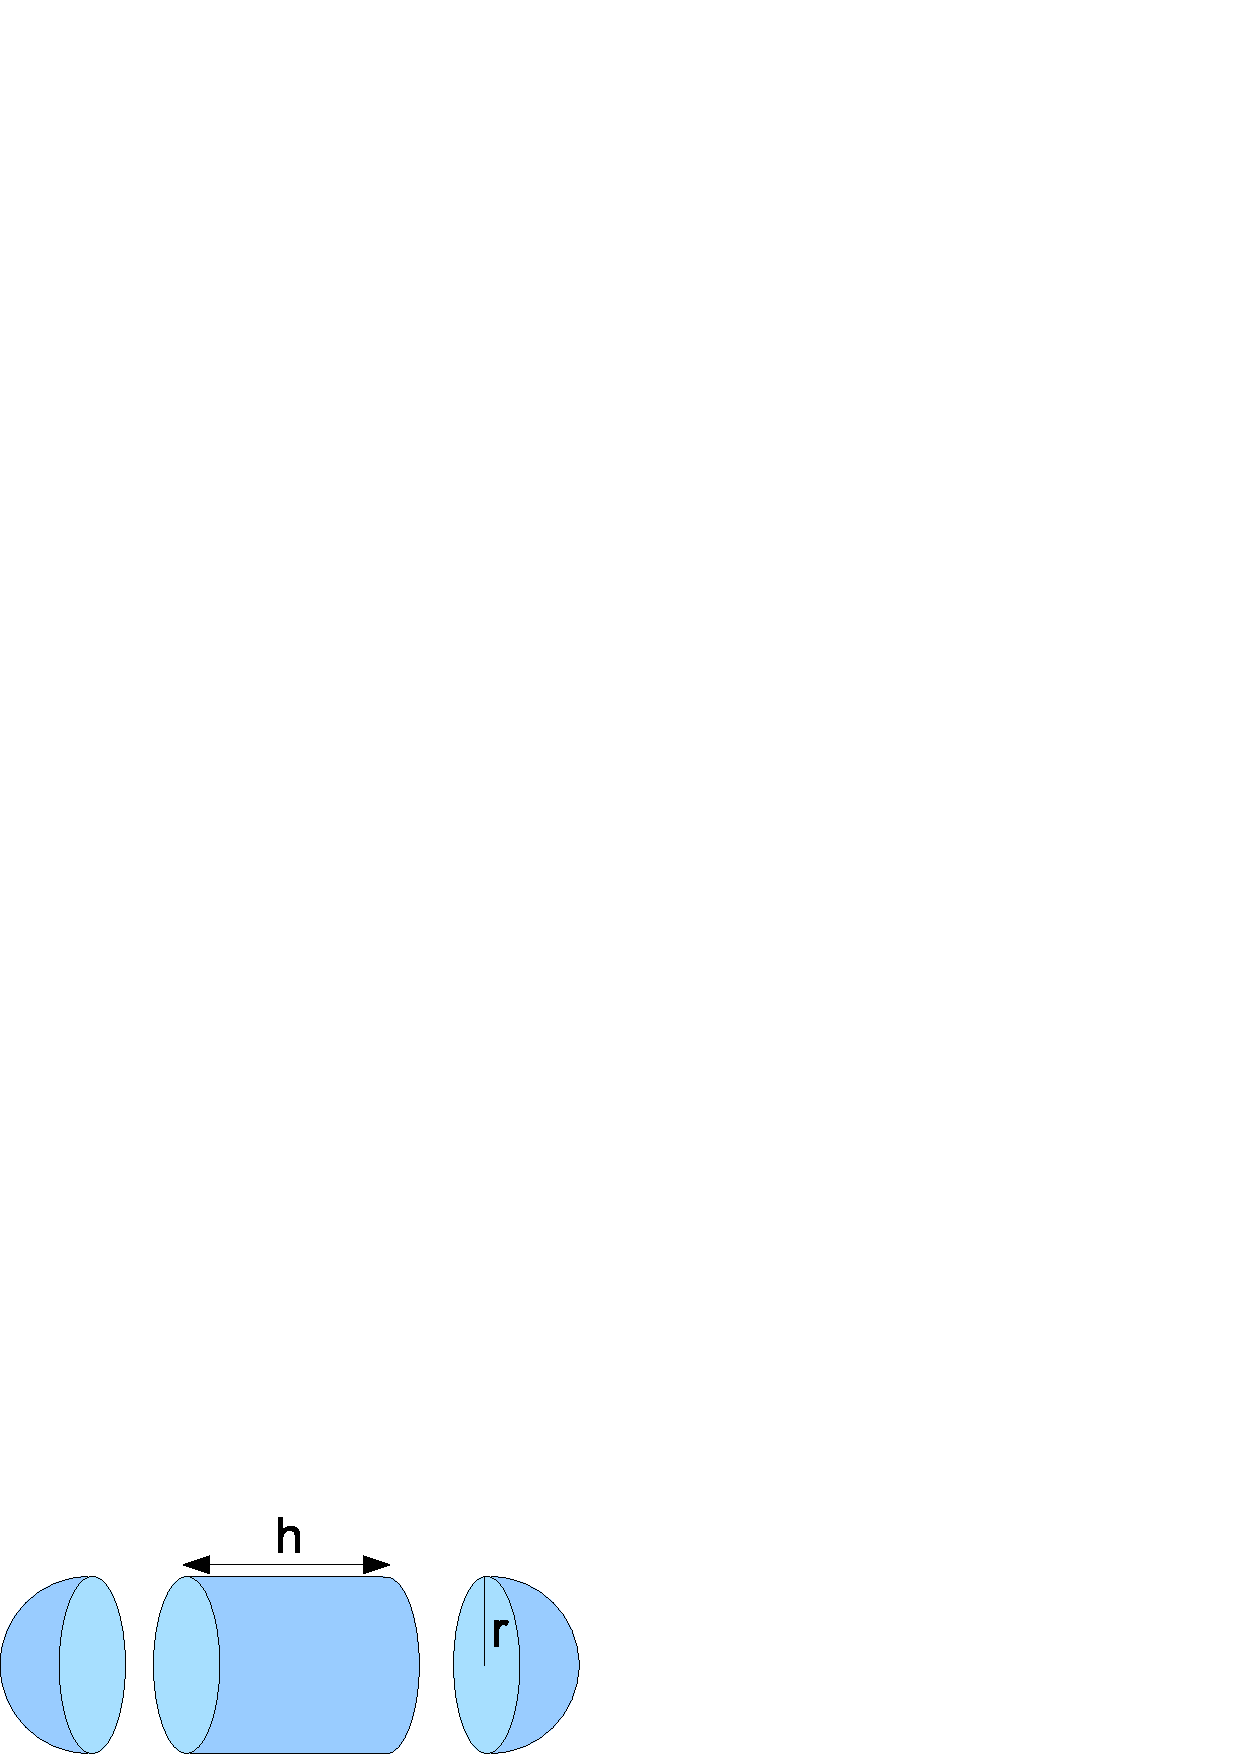
\includegraphics[scale=0.4]{img/capsula-ext-6}
\]
así que su volumen es
\[
V(r,h) = \pi r^2 h + \frac{4}{3}\pi r^3,
\]  
y su superficie
\[
S(r,h) = 2\pi r h +4 \pi r^2.
\]
Como el volumen  debe ser $0.8$ cm$^3$ tenemos que
\[
V(r,h) = \pi r^2 h + \frac{4}{3}\pi r^3 = 0.8 \Leftrightarrow h = \frac{0.8-4/3\pi r^3}{\pi r^2},
\]
y sustituyendo en la fórmula de superficie tenemos
\[
S(r) = 2\pi r \frac{0.8-4/3 \pi r^3}{\pi r^2} +4 \pi r^2 = \frac{1.6-8/3\pi r^2}{r}+4\pi r^2 = \frac{1.6}{r}-\frac{8}{3}\pi r^2 +4\pi r^2 = \frac{1.6}{r^2}+\frac{4}{3}\pi r^2
\]
Como queremos que la superficie de la cápsula sea mínima, tenemos que buscar el mínimo de esta función. Para ello, calculamos primero los puntos críticos que anulan su derivada:
\[
\frac{dS}{dr} = -\frac{1.6}{r^2}+\frac{4}{3}\pi2r = 0 \Leftrightarrow \frac{1.6}{r^2} = \frac{8}{3}\pi r \Leftrightarrow \frac{8}{3}\pi r^3 = 1.6 \Leftrightarrow r^3 = \frac{1.6}{8/3 \pi} = 0.1910 \Leftrightarrow r = \sqrt[3]{0.1910} = 0.5759
\]
y por tanto la altura será
\[
h = \frac{0.8-4/3\pi r^3}{\pi r^2} = \frac{0.8-4/3\pi 0.5759^3}{\pi 0.5759^2} = 0.
\]
Esto quiere decir, que realmente no habría cilindro, y por tanto para que la supercie sea mínima la cápsula debería tener forma de esfera. 

Sólo falta comprobar que el punto anterior es realmente un punto de mínimo. Para ello podemos utilizar la segunda derivada
\[
\frac{d^2S}{dr^2} = \frac{d}{dr}\left(-\frac{1.6}{r^2}+\frac{8}{3}\pi r\right) = \frac{1.6\cdot 2r}{r^4}+\frac{8}{3}\pi = \frac{3.2}{r^3}+\frac{8}{3}\pi. 
\]
y sustituyendo en el punto anterior tenemos
\[
\frac{d^2S}{dr^2}(0.5759) =  \frac{3.2}{0.5759^3}+\frac{8}{3}\pi = 25.13 >0,
\]
que al tener signo positivo indica que efectivamente se trata de un mínimo.
}

\newproblem{ext-7}{gen}{*}
%ENUNCIADO
{Sea $f(x)$ una función cuya derivada vale:
\[
f'(x) = \frac{(2-x) e^{-\frac{x^2}{2}+2x-2}}{\sqrt{2\pi}}
\]
Se pide:
\begin{enumerate}
\item Estudiar el crecimiento de $f$.
\item Calcular los valores de $x$ en los que $f$ tiene extremos relativos.
\item Estudiar la concavidad de $f$.
\item Calcular los valores de $x$ en los que $f$ tiene puntos de inflexión.
\end{enumerate}
}
%SOLUCIÓN
{\begin{enumerate}
\item Creciente en $x<2$ y decreciente en $x>2$.
\item Máximo relativo en $x=2$.
\item Cóncava en $(-\infty,1)$ y $(3,\infty)$. Convexa en $(1,3)$.
\item Puntos de inflexión en $x=1$ y $x=3$.
\end{enumerate}
}
%RESOLUCIÓN
{
}


\newproblem{ext-8}{qui}{}
%ENUNCIADO
{La velocidad $v$ de una reacción irreversible $A+B\rightarrow AB$ es función de la concentración $x$ del producto $AB$ y puede expresarse según la ecuación
\[
v(x) = 4(3-x)(5-x).
\]
¿Qué valor de $x$ maximiza la velocidad de reacción?
}
%SOLUCIÓN
{Ninguno.
}
%RESOLUCIÓN
{
}


\newproblem{ext-9}{amb}{}
%ENUNCIADO
{La cantidad de trigo en una cosecha $C$ depende del nivel de nitrógeno en el suelo $n$ según la ecuación
\[
C(n) = \frac{n}{1+n^2},\quad n\geq 0. 
\]
¿Para qué nivel de nitrógeno se obtendrá la mayor cosecha de trigo?
}
%SOLUCIÓN
{$n=1$.
}
%RESOLUCIÓN
{
}


\newproblem{ext-10}{amb}{}
%ENUNCIADO
{Existen organismos que se reproducen una sóla vez en su vida como por ejemplo los salmones. 
En este tipo de especies, la velocidad de incremento per cápita $v$, que mide la capacidad reproductiva, depende de la edad $x$ según la ecuación
\[
v(x) = \frac{\log(p(x)h(x))}{x},
\] 
donde $p(x)$ es la probabilidad de sobrevivir hasta la edad $x$ y $h(x)$ es el número de nacimientos de hembras a la edad $x$. 
Calcular la edad óptima de reproducción, es decir, el valor que maximice $v$, para $p(x)=e^{-0.1x}$ y $h(x)=4x^{0.9}$.}
%SOLUCIÓN
{$x=0.58$ años.
}
%RESOLUCIÓN
{
}


\newproblem{ext-12}{amb}{}
%ENUNCIADO
{La sensibilidad de $S$ de un organismo ante un fármaco depende de la dosis $x$ suministrada según la relación
\[
S(x) = x(C-x),
\]
siendo $C$ la cantidad máxima del fármaco que puede suministrarse, que depende de cada individuo. 
Hallar la dosis $x$ para la que la sensibilidad es máxima. 
}
%SOLUCIÓNsensibilidad
{$x=C/2$.
}
%RESOLUCIÓN
{
}

% Autor: Alfredo Sánchez Alberca (asalber@ceu.es)

\newproblem*{tay-1}{gen}{}
%ENUNCIADO
{Dada la función $f(x)=\sqrt{x+1}$ se pide:
\begin{enumerate}
\item  El polinomio de Taylor de cuarto grado de $f$ en $x=0$.
\item  Calcular un valor aproximado de $\sqrt{1.02}$ utilizando un polinomio de segundo grado y otro utilizando un polinomio de cuarto grado. Dar una cota del error cometido en cada caso.
\end{enumerate}
}


\newproblem{tay-2}{gen}{}
%ENUNCIADO
{Dada la función $f(x)=\sen x$, se pide:
\begin{enumerate}
\item  Obtener el polinomio de Taylor de tercer grado de $f$ en el punto $x=\pi/6$ y usarlo para aproximar $\sen\dfrac{1}{2}$ dando una cota del error cometido.
\item  Dar una aproximación de $\sen\dfrac{1}{2}$ usando un el polinomio de Taylor de quinto grado en el punto $x=0$, acotando el error cometido.
\end{enumerate}
}
%SOLUCIÓN
{
\begin{enumerate}
\item $P^3_{f,\pi/6}(x) = \frac{1}{2}+\frac{\sqrt{3}}{2}(x-\pi/6)-\frac{1}{4}(x-\pi/6)^2-\frac{\sqrt{3}}{12}(x-\pi/6)^3$.\\
$\sen 1/2 \approx P^3_{f,\pi/6}(1/2) = 0.4794255322$.\\
$|R^3_{f,\pi/6}(1/2)|\leq 6.46\cdot 10^{-9}$.
\item $P^5_{f,0}(x) = x -\frac{1}{6} x^3 + \frac{1}{120}x^5$.\\
$\sen 1/2 \approx P^5_{f,0}(1/2) = 0.4794270833$.\\
$|R^5_{f,0}(1/2)|\leq 2.170\cdot 10^{-5}$.
\end{enumerate}
}
%RESOLUCIÓN
{
}


\newproblem{tay-3}{gen}{}
%ENUNCIADO
{Obtener la fórmula de Taylor de segundo orden de la función $f(x)=\sqrt[3]{x}$ en un entorno del punto $x=1$.
}
%SOLUCIÓN
{$P^2_{f,1}(x) = 1+\frac{1}{3}(x-1)-\frac{2}{18}(x-1)^2$. 
}
%RESOLUCIÓN
{
}


\newproblem{tay-4}{gen}{}
%ENUNCIADO
{Calcular el polinomio de McLaurin de tercer grado para la función $f(x)=\arcsen x$.
}
%SOLUCIÓN
{$P^3_{f,0}(x) = x+\frac{1}{6}x^3$. 
}
%RESOLUCIÓN
{
}


\newproblem*{tay-5}{gen}{}
%ENUNCIADO
{Calcular $\cos 1$ con un error menor de $10^{-7}$ usando aproximaciones de Taylor.
}


\newproblem{tay-6}{gen}{*}
%ENUNCIADO
{Dadas las funciones
$f(x)=e^x$ y $g(x)=\cos x$, se pide:
\begin{enumerate}
   \item  Calcular los polinomios de McLaurin de segundo grado para $f$
   y $g$.

   \item  Utilizar los polinomios anteriores para calcular
   \[ \lim_{x\rightarrow 0}\frac{e^x-\cos x}{x}.\]
\end{enumerate}
}
%SOLUCIÓN
{\begin{enumerate}
\item $P^2_{f,0}(x) = 1+x+\frac{1}{2}x^2$ y $P^2_{g,0}(x) = 1-\frac{1}{2}x^2$.
\item $\lim_{x\rightarrow 0}\frac{e^x-\cos x}{x} = \lim_{x\rightarrow 0}\frac{x+x^2}{x} = 1$. 
\end{enumerate}
}
%RESOLUCIÓN
{
}


\newproblem{tay-7}{far}{*}
%ENUNCIADO
{La función $C(t)$ da la concentración (en mg/dl) de un fármaco en el torrente sanguíneo en función del tiempo (en horas):
\[
C(t) = \frac{1}{{1 + e^{-2t}}}
\]
\begin{enumerate}
\item Calcular el polinomio de Mc Laurin de orden 3.

\item Utilizando el polinomio anterior, calcular aproximadamente la concentración del fármaco transcurridos 15 minutos.
\end{enumerate}
}
%SOLUCIÓN
{
\begin{enumerate}
\item $P_{C,0}^3(t)=\frac{1}{2}+\frac{1}{2}t+0\frac{t^2}{2!}-1\frac{t^3}{3!}=\frac{1}{2}+\frac{1}{2}t-\frac{1}{6}t^3$.
\item $P_{C,0}^3(0.25)= 0.6223958333 \mbox{ mg/dl}$.
\end{enumerate}
}
%RESOLUCIÓN
{\begin{enumerate}
\item
La fórmula del polinomio de Mc Laurin de orden 3 para la función $C(t)$ es:
\begin{equation}
\label{e:mclaurin}
P_{C,0}^3(t)=C(0)+\frac{dC}{dt}(0)t+\frac{d^2C}{dt^2}(0)\frac{t^2}{2!}+\frac{d^3C}{dt^3}(0)\frac{t^3}{3!}
\end{equation}
Necesitamos calcular las tres primeras derivadas:
\begin{align*}
\frac{dC}{dt} &= \frac{2e^{-2t}}{(1+e^{-2t})^2},\\
\frac{d^2C}{dt^2} &=
\frac{\frac{d}{dt}(2e^{-2t})(1+e^{-2t})^2-2e^{-2t}\frac{d}{dt}(1+e^{-2t})^2}{(1+e^{-2t})^4} =\\
&= \frac{-4e^{-2t}(1+e^{-2t})^2- 2e^{-2t}2(1+e^{-2t})(-2e^{-2t})}{(1+e^{-2t})^4}
= \frac{-4e^{-2t}+4e^{-4t}}{(1+e^{-2t})^3},\\
\frac{d^3C}{dt^3}
&=
\frac{\frac{d}{dt}(-4e^{-2t}1+4e^{-4t})(1+e^{-2t})^3-(-4e^{-2t}+4e^{-4t})\frac{d}{dt}(1+e^{-2t})^3}{(1+e^{-2t})^6}=\\
&=
\frac{(8e^{-2t}-16e^{-4t})(1+e^{-2t})^3-(-4e^{-2t}+4e^{-4t})3(1+e^{-2t})^2(-2e^{-2t})}{(1+e^{-2t})^6}=\\
&=
\frac{(8e^{-2t}-16e^{-4t})(1+e^{-2t})-(-4e^{-2t}+4e^{-4t})(-6e^{-2t})}{(1+e^{-2t})^4}=\\
&=
\frac{(8e^{-2t}-8e^{-4t}-16e^{-6t})-(24e^{-4t}-24e^{-6t})}{(1+e^{-2t})^4}=\\
&=
\frac{8e^{-2t}-32e^{-4t}+8e^{-6t}}{(1+e^{-2t})^4}.
\end{align*}
Sustituyendo para $t=0$ tenemos:
\begin{align*}
C(0)&= \frac{1}{1+e^{-2\cdot 0}}=\frac{1}{2},\\
\frac{dC}{dt}(0) &= \frac{2e^{-2\cdot 0}}{(1+e^{-2\cdot 0})^2} = \frac{2}{2^2}=\frac{1}{2},\\
\frac{d^2C}{dt^2}(0) &= \frac{-4e^{-2\cdot 0}+4e^{-4\cdot 0}}{(1+e^{-2\cdot
0})^3} = \frac{-4+4}{2^3}= 0,\\
\frac{d^3C}{dt^3}(0)&=\frac{(8e^{-2\cdot 0}-32e^{-4\cdot 0}+8e^{-6\cdot 0})}{(1+e^{-2\cdot 0})^4}=\frac{8-32+8}{16}=-1.
\end{align*}

Y por último, sustituyendo en la ecuación \ref{e:mclaurin} llegamos al polinomio
\[
P_{C,0}^3(t)=\frac{1}{2}+\frac{1}{2}t+0\frac{t^2}{2!}-1\frac{t^3}{3!}=\frac{1}{2}+\frac{1}{2}t-\frac{1}{6}t^3.
\]

\item La concentración del fármaco transcurridos 15 minutos ($0.25$ horas) es aproximadamente
\[
C(0.25)\approx P_{C,0}^3(0.25)= \frac{1}{2}+\frac{1}{2}0.25-\frac{1}{6}0.25^3= 0.6223958333 \mbox{ mg/dl}.
\]
\end{enumerate}
}


\newproblem{tay-8}{gen}{*}
%ENUNCIADO
{Obtener el desarrollo en serie de Taylor hasta orden tres en el punto $1$ de la función 
\[f(x) = \ln\sqrt{\dfrac{x^2+1}{2}}.\]
Utilizar el polinomio obtenido calcular una aproximación de $\ln\sqrt{1.22}$ y acotar el error cometido.
}
%SOLUCIÓN
{$P^3_{f,1}(x) = \frac{1}{2}(x-1)-\frac{1}{12}(x-1)^3$.\\
$\ln\sqrt{1.22} \approx P^3_{f,1}(1.2) = 0.0993333$.\\
$|R^3_{f,1}(1.2)|\leq 1.25\cdot 10^{-4}$.

}
%RESOLUCIÓN
{
}


\newproblem{tay-9}{gen}{*}
%ENUNCIADO
{Dada la función $f(x)=\arctg(x/2)$ se pide:
\begin{enumerate}
\item Calcular el polinomio de Mc Laurin de orden 3.
\item Utilizar el polinomio anterior para aproximar $\arctg 0.05$.
\item Dar una cota del error cometido.
\end{enumerate}
}
%SOLUCIÓN
{\begin{enumerate}
\item $P^3_{f,0}(x) =  \frac{1}{2}x-\frac{1}{24}x^3$.
\item $\arctan 0.05 \approx P^3_{f,0}(0.1) = 0.0499583333$.
\item $|R^3_{f,0}(0.1)|\leq 3.08\cdot 10^{-7}$.
\end{enumerate}
}
%RESOLUCIÓN
{
}


\newproblem{tay-10}{gen}{*}
%ENUNCIADO
{Dada la función $f(x)=\dfrac{1}{1-x}$ con $x\neq 1$, se pide:
\begin{enumerate}
\item Calcular el polinomio de Mc Laurin de $f$ de grado 4.
\item Calcular el polinomio de Mc Laurin de $f$ de grado $n$.
\item Calcular el resto de Lagrange para el polinomio de grado $n$ en el punto $x=0.03$.
\item ¿Hasta qué grado tendríamos que llegar para conseguir una aproximación de $f(0.03)$ con un error menor de $10^{-10}$?
\end{enumerate}
}
%SOLUCIÓN
{\begin{enumerate}
\item $P^4_{f,0}(x) = 1 + x + x^2 + x^3 + x^4$.
\item $P^n_{f,0}(x) = 1 + x + x^2 + \cdots + x^n$.
\item $R^n_{f,0}(0.03) = \frac{0.03^{n+1}}{(1-t)^{n+2}} \ t\in(0,0.03)$.
\item $|R^n_{f,0}(0.03)| \leq \frac{0.03^{n+1}}{(0.97)^{n+2}}\leq 10^{-10}$ para $n\geq 6$.
\end{enumerate}
}
%RESOLUCIÓN
{
}


\newproblem{tay-11}{gen}{*}
%ENUNCIADO
{Dada la función $f(x)=\tg(x/2)$, se pide:
\begin{enumerate}
\item Aproximar $\tg(0.1)$ mediante un polinomio de Taylor de grado 3 para la función $f$.
\item Dar una cota del error cometido.
\end{enumerate}
}
%SOLUCIÓN
{
\begin{enumerate}
\item $T_3 (f,0)(0.2) = 0.1003333$.
\item ${\rm Error} \le 0.00033$.
\end{enumerate}
}
%RESOLUCIÓN
{\begin{enumerate}
\item Sabemos que el desarrollo de Taylor de grado 3 de una función
$f$,  centrado en $a$ y en función de $x$ viene dado por:
\[
T_3 (f,a)(x) = f(a) + f'(a)(x - a) + \frac{{f''(a)}}{2}(x - a)^2  +
\frac{{f'''(a)}}{6}(x - a)^3
\]
y que el valor de la función en un cierto $x_0$, próximo a $a$,
puede calcularse de forma aproximada mediante:
\[
f(x_0 ) \approx T_3 (f,a)(x_0 )
\]
En nuestro caso, la función $f(x)= \tg x/2$ y debemos aproximar el
valor de $\tg 0.1$. Por lo tanto:
\[
\tg 0.1 = \tg \frac{{x_0 }}{2} \Leftrightarrow x_0  = 0.2
\]
Y como valor de $a$ (punto en el que centramos el polinomio de
Taylor) podemos tomar 0, ya que está lo suficientemente próximo a
$0.2$ como para que la aproximación sea buena, además de simplificar
notablemente los cálculos. Es decir, vamos a calcular el polinomio
de Mc Laurin.

Entre las múltiples expresiones para la derivada de la tangente
(como cociente de senos y cosenos, con la secante y también con la
propia tangente), posiblemente la más cómoda para hacer derivadas de
orden superior es:
\[
f(x) = \tg (u(x)) \Rightarrow f'(x) = \left( {1 + \tg ^2 (u(x))}
\right)u'(x)
\]
Aplicado a nuestra función:
\[
f(x) = \tg \frac{x}{2}
\]
\[
f'(x) = \left( {1 + \tg ^2 \frac{x}{2}} \right)\frac{1}{2} =
\frac{1}{2} + \frac{1}{2}\tg ^2 \frac{x}{2}
\]

Procediendo de forma similar con las derivadas de segundo y tercer
orden, obtenemos:
\[
f''(x) = \frac{1}{2}\tg \frac{x}{2} + \frac{1}{2}\tg ^3
\frac{x}{2}
\]
\[
f'''(x) = \frac{1}{4} + \tg ^2 \frac{x}{2} + \frac{3}{4}\tg ^4
\frac{x}{2}
\]
Por lo tanto:
\[
f(0) = 0;\;f'(0) = 1/2;\;f''(0) = 0;\;f'''(0) = 1/4
\]
Con ello, el polinomio de Mac Laurin buscado es:
\[
T_3 (f,0)(x) = \frac{1}{2}x + \frac{1}{{24}}x^3
\]

Y la aproximación buscada vale:
\[
\tg 0.1 \approx T_3 (f,0)(0.2) = \frac{1}{2}\;0.2 +
\frac{1}{{24}}\;0.2^3  = 0.1003333
\]
Para comprobar que la aproximación obtenida es correcta, mediante
calculadora, utilizando como unidad angular el radián, obtenemos:
$\tg 0.1=0.1003346$


\item Sabemos que el error cometido con la anterior aproximación es
igual al valor absoluto del resto, y que este último viene dado por
la fórmula:
\[
R_n (f,a)(x) = \frac{{f^{(n + 1} (t)}}{{(n + 1)!}}(x - a)^{n + 1}
\]
donde $t$ pertenece al intervalo $(a,x)$ si $x>a$, o a $(x,a)$ si
$a>x$.
En nuestro caso:
\[
R_3 (f,0)(0.2) = \frac{{f^{(4} (t)}}{{4!}}(0.2)^{4}
\]
Si tenemos en cuenta que la derivada cuarta vale:
\[
f^{(4} (x) = \tg \frac{x}{2} + \frac{5}{2}\tg ^3 \frac{x}{2} +
\frac{3}{4}\tg ^5 \frac{x}{2} \Rightarrow f^{(4} (t) = \tg
\frac{t}{2} + \frac{5}{2}\tg ^3 \frac{t}{2} + \frac{3}{4}\tg ^5
\frac{t}{2}
\]
obtenemos:
\[
R_3 (f,0)(0.2) = \frac{{\tg \frac{t}{2} + \frac{5}{2}\tg ^3
\frac{t}{2} + \frac{3}{4}\tg ^5 \frac{t}{2}}}{{24}}\,(0.2)^4 ;\quad
t \in (0,\;0.2)
\]
Por lo tanto el error cometido vale:
\[
\left| {\frac{{\tg \frac{t}{2} + \frac{5}{2}\tg ^3 \frac{t}{2} +
\frac{3}{4}\tg ^5 \frac{t}{2}}}{{4!}}\,(0.2)^4 } \right|;\quad t
\in (0,\;0.2)
\]
Y nos piden que acotemos el error, es decir, que encontremos una
cierta cantidad tal que se demuestre que el error es menor o igual
que esa cantidad. Para ello, nos damos cuenta de que la función
tangente, e igualmente la tangente al cubo o a la quinta potencia,
son funciones crecientes en el intervalo $(0,\,0.2)$ y, por lo
tanto, el error alcanzará su máximo valor posible cuando $t$ sea un
valor muy próximo a $0.2$. No obstante obtenemos un error en cuya
expresión aparece de nuevo la tangente de $0.1$, y no tiene ningún
sentido utilizar la calculadora para calcular la tangente de $0.1$
presente en el resto, cuando precisamente es la tangente de $0.1$ lo
que pretendemos calcular mediante el polinomio de Taylor. No
obstante, podemos utilizar otras cotas menos precisas pero que
supongan cálculos fácilmente realizables sin necesidad de
calculadora, y evitando a la vez el que la tangente de $0.1$
aparezca en el error. Por ejemplo, la más sencilla se obtiene
considerando que en el intervalo $(0,\,0.2)$ $\tg(t/2)\leq 1$, e
igualmente la tangente cubo o a la quinta potencia.

Teniendo en cuenta lo anterior:
\[
{\rm Error} \le \frac{{(0.2)^4 }}{{4!}}\left| {1 + \frac{5}{2} +
\frac{3}{4}\,} \right| = 0.00033
\]
Una cota más precisa se obtiene tomando, por ejemplo, $t=\pi/3$, tal
que la tangente de $\pi/6$ sí que tiene un valor fácilmente
calculable (sin calculadora):
\[
\tg \frac{\pi }{6} = \frac{{1/2}}{{\sqrt 3 /2}} = \frac{{\sqrt 3
}}{3}
\]
Con ello, la cota para el error cometido vale:
\[
{\rm Error} \le \frac{{(0.2)^4 }}{{4!}}\left| {1\frac{{\sqrt 3 }}{3}
+ \frac{5}{2}\left( {\frac{{\sqrt 3 }}{3}} \right)^3  +
\frac{3}{4}\left( {\frac{{\sqrt 3 }}{3}} \right)^5 \,} \right| =
0.000077
\]
\end{enumerate}
}


\newproblem{tay-12}{gen}{*}
%ENUNCIADO
{Dada  la función $f(x) = 2\sqrt[3]{{1 + x}}$, se pide:
\begin{enumerate}
\item Hallar el polinomio de Mc Laurin de tercer grado de la función. 
\item Utilizar el polinomio obtenido en el apartado anterior para calcular un valor aproximado de $\sqrt[3]{9}$.
\item Dar una cota del error cometido.
\end{enumerate}
}
%SOLUCIÓN
{\begin{enumerate}
\item $P(3,f,0)(x)=2+\frac{2}{3}x-\frac{2}{9}x^2+\frac{10}{81}x^3$.
\item $P(3,f,0)(0.125)= 2.080102258$.
\item $|R_{3,f,0}(0.125)| \leq 2.00938\cdot 10^{-5}$.
\end{enumerate}
}
%RESOLUCIÓN
{\begin{enumerate}
\item   La fórmula del polinomio de Mc Laurin de orden $3$ para la 
    función $f$ es
\begin{equation}
    P_{3,f,0} (x)= f(0)+ 
    f'(0)x+\frac{f''(0)}{2!}x^2+\frac{f'''(0)}{3!}x^3,
    \label{McLaurin}
\end{equation}
de modo que tenemos que calcular hasta la tercera derivada de $f$ en el 0.
\[ \renewcommand{\arraystretch}{2}
    \begin{array}{lll}
        f(x)=2\sqrt[3]{{1 + x}}=2(1+x)^{1/3}, & \quad \quad & f(0)=2(1+0)^{1/3}=2,  \\
        f'(x)=2\dfrac{1}{3}(1+x)^{-2/3}=\dfrac{2}{3}(1+x)^{-2/3}, &  & f'(0)=\dfrac{2}{3}(1+0)^{-2/3}=\dfrac{2}{3},\\
        f''(x)=\dfrac{2}{3}\dfrac{-2}{3}(1+x)^{-5/3}=\dfrac{-4}{9}(1+x)^{-5/3}, &  & f''(0)=\dfrac{-4}{9}(1+0)^{-5/3}=\dfrac{-4}{9},\\
        f'''(x)=\dfrac{-4}{9}\dfrac{-5}{3}(1+x)^{-8/3}=\dfrac{20}{27}(1+x)^{-8/3}, &  & f'''(0)=\dfrac{20}{27}(1+0)^{-8/3}=\dfrac{20}{27},
     \end{array}  
\]
Sustituyendo estos valores en la ecuación \ref{McLaurin}, 
obtenemos el polinomio que nos piden
\[ 
P(3,f,0)(x)= 2+\frac{2}{3}x+\frac{-4/9}{2}x^2+\frac{20/27}{6}x^3=
2+\frac{2}{3}x-\frac{2}{9}x^2+\frac{10}{81}x^3.      
\]    

\item Primero averiguamos en qué punto la función vale $\sqrt[3]{9}$. 
\[
f(x)=2\sqrt[3]{1+x}=\sqrt[3]{9} \Leftrightarrow (2\sqrt[3]{1+x})^3=(\sqrt[3]{9})^3 \Leftrightarrow
2^3(1+x)=9 \Leftrightarrow 8+8x=9 \Leftrightarrow x=\frac{1}{8}=0.125.
\]
Calculando el polinomio anterior en este punto tenemos
\[ 
\sqrt[3]{9}\approx P(3,f,0)(0.125)= 2+\frac{2}{3}0.125-\frac{2}{9}0.125^2+\frac{10}{81}0.125^3=2.080102258.      
\]

\item El error cometido en la aproximación anterior nos lo da el resto de Taylor, que en la forma
Lagrange es
\[
R_{3,f,0}(x)=\frac{f^{iv}(t)}{4!}x^4=\frac{\frac{160}{81} (1+t)^{-11/3}}{24}x^4 = \frac{20}{243}\frac{1}{(1+t)^{11/3}} x^4 \quad t\in(0,x),
\]
En el punto $x=0.125$ donde hemos calculado la aproximación, vale
\[
R_{3,f,0}(0.125)=\frac{20}{243}\frac{1}{(1+t)^{11/3}} 0.125^4= 2.00938\cdot 10^{-5}\frac{1}{(1+t)^{11/3}} \quad t\in(0\,,\,0.125).
\]
Para acotar el resto, basta con calcular el máximo de esta función en el
intervalo $(0\,,\,0.125)$. Puesto que la función $1/(1+t)^{11/3}$ es decreciente en dicho intervalo,
el máximo se alcanza en el extremo inferior del intervalo, es decir,
$t=0$. Así pues, tenemos la siguiente cota
\[
|R_{3,f,0}(0.125)|=|2.00938\cdot 10^{-5}\frac{1}{(1+t)^{11/3}}|\leq
|2.00938\cdot 10^{-5}\frac{1}{(1+0)^{11/3}}|=2.00938\cdot 10^{-5}.
\]
\end{enumerate}
}


\newproblem{tay-13}{gen}{*}
%ENUNCIADO
{Dada la función: $f(x) = \dfrac{2} {{\sqrt {3x+ 1} }}$
\begin{enumerate}
\item Obtener el polinomio de Mac Laurin de tercer grado.
\item Calcular el valor aproximado de $\dfrac{2}{1,3}$ empleando el polinomio anterior.
\end{enumerate}
}
%SOLUCIÓN
{\begin{enumerate}
\item $P(3,f,0)(x)= 2-3x+\frac{27}{4}x^2-\frac{135}{8}x^3$.
\item $\frac{2}{1.3}\approx P(3,f,0)(0.23)=1.461756910$.
\end{enumerate}
}
%RESOLUCIÓN
{\begin{enumerate}
\item   La fórmula del polinomio de Mc Laurin de orden $3$ para la función $f$ es
\begin{equation}
P_{3,f,0} (x)= f(0)+ f'(0)x+\frac{f''(0)}{2!}x^2+\frac{f'''(0)}{3!}x^3,
\label{McLaurin}
\end{equation}
de modo que tenemos que calcular hasta la tercera derivada de $f$ en el 0.
\[ \renewcommand{\arraystretch}{2}
    \begin{array}{ll}
        f(x)=\dfrac{2}{\sqrt{3x+1}}= 2(3x+1)^{-1/2}, & f(0)=2(3\cdot 0+1)^{-1/2}=2,  \\
        f'(x)=2\dfrac{-1}{2}(3x+1)^{-3/2}3=-3(3x+1)^{-3/2}, &  f'(0)=-3(3\cdot 0+1)^{-3/2}=-3,\\
        f''(x)=-3\dfrac{-3}{2}(3x+1)^{-5/2}3=\dfrac{27}{2}(3x+1)^{-5/2}, &  f''(0)=\dfrac{27}{2}(3\cdot 0+1)^{-5/2}=\dfrac{27}{2},\\
        f'''(x)=\dfrac{27}{2}\dfrac{-5}{2}(3x+1)^{-7/2}3=\dfrac{-405}{4}(3x+1)^{-7/2}, & f'''(0)=\dfrac{-405}{4}(3\cdot 0+1)^{-7/2}=\dfrac{-405}{4},
     \end{array}  
\]
Sustituyendo estos valores en la ecuación \ref{McLaurin}, obtenemos el polinomio que nos piden
\[ 
P(3,f,0)(x)= 2-3x+\frac{27/4}{2!}x^2-\frac{405/24}{3!}x^3=
2-3x+\frac{27}{4}x^2-\frac{135}{8}x^3.      
\]    

\item Primero averiguamos en qué punto la función vale $2/1.3$. 
\[
f(x)=\frac{2}{\sqrt{3x+1}}=\frac{2}{1.3} \Leftrightarrow \sqrt{3x+1}=1.3 \Leftrightarrow
3x+1=1.3^2=1.69 \Leftrightarrow x=\frac{0.69}{3}=0.23.
\]
Calculando el polinomio anterior en este punto tenemos
\[ 
\frac{2}{1.3}\approx P(3,f,0)(0.23)= 2-3\cdot 0.23+\frac{27}{4}0.23^2-\frac{135}{8}0.23^3=1.461756910.      
\]
\end{enumerate}
}


\newproblem*{tay-14}{gen}{*}
%ENUNCIADO
{Sea la función
\[
f(x) = 2\sqrt[4]{{1 + x}}
\]
\begin{enumerate}
\item Calcular su desarrollo de Mc Laurin de orden 3.
\item Utilizar el desarrollo anterior para calcular de forma aproximada: $\sqrt[4]{{16,16}}$.
\item Acotar el error cometido con la aproximación anterior.
\end{enumerate}
}


\newproblem*{tay-15}{gen}{*}
%ENUNCIADO
{
Sea la función $f(x)=x^{x}.$
\begin{enumerate}
\item  Calcular su polinomio de Taylor de segundo orden, centrado en $x=1$.
\item  Aproximar con dicho polinomio el valor de: $1.1^{1.1}$.
\end{enumerate}
}


\newproblem*{tay-16}{gen}{*}
%ENUNCIADO
{Para la función:
\[
f(x)=\sqrt[3]{1+2x}
\]
Calcular:
\begin{enumerate}
\item  Su polinomio de Taylor de tercer orden centrado en 0.
\item  El valor aproximado de $\sqrt[3]{1.2}$ mediante el polinomio de Taylor calculado anteriormente.
\item  Acotar el error cometido mediante dicha aproximación.
\end{enumerate}
}


\newproblem*{tay-17}{gen}{*}
%ENUNCIADO
{Teniendo en cuenta que $\sen (2x)=2\sen x \cos x$ y los desarrollos de McLarin de las funciones $\sen x$ y $\cos x$, ¿cuál será el desarrollo de Mc Laurin de orden 3 para la función $\sen (2x)$?

Calcular directamente el desarrollo de Mc Laurin de orden 3 de la función $\sen (2x)$ para comprobar el resultado obtenido en el apartado anterior.
}


\newproblem*{tay-18}{gen}{*}
%ENUNCIADO
{En los libros de Cálculo se afirma que la función binómica, $(1+x)^p$, puede desarrollarse desarrollada mediante una serie de sumandos de la forma:
\[
\left( {1 + x} \right)^p  = 1 + px + \frac{{p(p - 1)}} {{2!}}x^2 + \frac{{p(p - 1)(p - 2)}} {{3!}}x^3  +  \cdots  + \frac{{p(p - 1) \cdots (p - k + 1)}} {{k!}}x^k
\]
para todo $x$ si $p$ es un entero no negativo.
\begin{enumerate}
\item Demostrar dicha fórmula hasta el término en $x^4$ mediante el desarrollo de Mc Laurin de orden 4.
\item Utilizar el resultado anterior para calcular de forma aproximada el valor de: $0.9^6$.
\end{enumerate}
}


\newproblem{tay-19}{gen}{*}
%ENUNCIADO
{La concentración de un fármaco en sangre, en mg/dl, en función del tiempo, en horas, viene dada por la expresión:
\[
C(t) = \ln \left( {\frac{{t^2  + 2t + 1}}{{2t + 1}}} \right)
\]
Se pide:
\begin{enumerate}
\item Calcular el polinomio de Mc Laurin de orden 3 de $C$.
\item Utilizar el polinomio anterior para dar el valor aproximado de la concentración al cabo de 15 minutos.
\item Calcular el polinomio de Taylor, centrado en 0, de orden 2 para la función:
\[
f(t) = 2\ln (t + 1) - \ln (2t + 1)
\]
\end{enumerate}
}
%SOLUCIÓN
{\begin{enumerate}
\item $P_{C,0}^3(t) = t^2-2t^3$.
\item $P_{C,0}^3(0.25) = 0.03125$.
\item $P_{f,0}^2(t) = t^2$.
\end{enumerate}}
%RESOLUCIÓN
{\begin{enumerate}
\item La ecuación del polinomio de Mc Laurin de orden 3 de $C$ es 
\begin{equation}
P_{C,0}^3(t) = C(0)+ C'(0)t + \frac{C''(0)}{2}t^2 + \frac{C'''(0)}{3!}t^3.
\end{equation}
Necesitamos calcular las 3 primeras derivadas, pero antes conviene simplificar la función 
\begin{align*}
C(t)&= \ln\left(\frac{t^2+2t+1}{2t+2}\right)= \ln(t^2+2t+1)-\ln(2t+1) =\\
&= \ln((t+1)^2) -\ln(2t+1) = 2\ln(t+1)-\ln(2t+1),\\
C'(t)&= \frac{2}{t+1}-\frac{2}{2t+1},\\
C''(t)&= \frac{-2}{(t+1)^2}+\frac{4}{(2t+1)^2},\\
C'''(t)&= \frac{4}{(t+1)^3}-\frac{16}{(2t+1)^3}
\end{align*}
Las derivadas en 0 valen
\begin{align*}
C(0)&=  2\ln(1)-\ln(1) = 0,\\
C'(0)&= \frac{2}{1}-\frac{2}{1}= 0,\\
C''(0)&= \frac{-2}{1^2}+\frac{4}{1^2} = 2,\\
C'''(t)&= \frac{4}{1^3}-\frac{16}{1^3} = -12.
\end{align*}
Y sustituyendo en la ecuación anterior llegamos al polinomio 
\[
P_{C,0}^3(t) = \frac{2}{2}t^2 - \frac{12}{3!}t^3 = t^2-2t^3.
\]

\item El valor de la función a los 15 minutos es $C(0.25)$ ya que las unidades del tiempo se consideran en horas. El valor aproximado de que da el polinomio en ese instante es
\[
P_{C,0}^3(0.25) = 0.25^2-2\cdot 0.25^3 = 0.03125.
\]

\item Según hemos podido comprobar al simplificar $C(t)$ resulta que $C(t)$ y $f(t)$ son la misma función, así que el polinomio de Mc Laurin de orden 2 es el mismo que el calculado en el primer apartado pero considerando sólo hasta el término de grado 2, es decir,
\[
P_{f,0}^2(t) = t^2.
\]
\end{enumerate}
}


\newproblem{tay-20}{gen}{}
%ENUNCIADO
{Dada la función $\dfrac{\sen x+\cos x}{2}$:
\begin{enumerate}
\item  Utilizar el polinomio de Mc Laurin de grado 3 para aproximar $\frac{\sen 1+\cos 1}{2}$.
\item  Utilizar el polinomio de Taylor de grado 2 en el punto $x_0 = \pi/2$ para aproximar $\frac{\sen 1+\cos 1}{2}$.
\item  Dar la cota de error cometida en ambas aproximaciones y decir cual es mejor.
\end{enumerate}
}
%SOLUCIÓN
{\begin{enumerate}
\item $P_0^3(x)=\frac{1}{2}+\frac{1}{2}x-\frac{1}{4}x^2-\frac{1}{12}x^3$ y $P_0^3(1)=\frac{2}{3}$.
\item $P_{\pi/2}^2(x)=\frac{1}{2}-\frac{1}{2}(x-\pi/2)-\frac{1}{4}(x-\pi/2)^2$ y  $P_{\pi/2}^2(1)= 0.70395$.
\item $|R_0^3(1)|\leq 0.04166$ y $|R_{\pi/2}^2(1)|\leq 0.03099$.
\end{enumerate}
}
%RESOLUCIÓN
{\begin{enumerate}
\item  El polinomio de Mc Laurin de grado 3 para $f(x)$ viene dado por la fórmula siguiente: 
\[
P_0^3(x)=f(0)+f^{\prime }(0)x+\frac{f^{\prime \prime }(0)}{2!}x^2+\frac{f^{\prime \prime \prime }(0)}{3!}x^3. 
\]

Calculamos las tres primeras derivadas de $f(x)$: 
\begin{align*}
f^{\prime }(x) &= \frac{\cos x-\sen x}{2}, \\
f^{\prime \prime }(x) &= \frac{-\ sen x-\cos x}{2}, \\
f^{\prime \prime \prime }(x) &= \frac{-\cos x+\sen x}{2}.
\end{align*}

Particularizando en $x=0$ tenemos: 
\begin{align*}
f(0) &= \frac{\sen 0+\cos 0}2=\frac{1}{2}, \\
f^{\prime }(0) &= \frac{\cos 0-\sen 0}{2}=\frac{1}{2}, \\
f^{\prime \prime }(0) &= \frac{-\sen 0-\cos 0}{2}=-\frac{1}{2}, \\
f^{\prime \prime \prime }(0) &= \frac{-\cos 0+\sen 0}{2}=-\frac{1}{2}.
\end{align*}

Por tanto, el polinomio de Mc Laurin que nos interesa es: 
\[
P_0^3(x)=\frac{1}{2}+\frac{1}{2}x-\frac{1}{4}x^2-\frac{1}{12}x^3.
\]

Para aproximar $f(1)=\frac{\sen 1+\cos 1}{2}$, tenemos que tomar $x=1$, y en ese punto, la aproximación que da el polinomio es: 
\[
P_0^3(1)=\frac{1}{2}+\frac{1}{2}-\frac{1}{4}-\frac{1}{12}=\frac{2}{3}.
\]

\item  El polinomio de Taylor de grado 2 en el punto $x_0=\pi/2$ para $f(x)$ viene dado por la fórmula siguiente: 
\[
P_{\pi /2}^2(x)=f(\pi /2)+f^{\prime }(\pi /2)(x-\pi /2)+\frac{f^{\prime\prime }(\pi /2)}{2!}(x-\pi /2)^2. 
\]

Particularizando en $x=\pi/2$ hasta la segunda derivada tenemos: 
\begin{align*}
f(\pi /2) &= \frac{\sen\pi/2+\cos \pi /2}{2} = \frac{1}{2} \\
f^{\prime }(\pi/2) &= \frac{\cos \pi /2-\sen\pi/2}{2} = -\frac{1}{2}, \\
f^{\prime \prime}(\pi/2) &= \frac{-\sen\pi/2-\cos\pi/2}{2} = -\frac{1}{2}.
\end{align*}

Por tanto, el polinomio de Taylor que nos interesa es: 
\[
P_{\pi/2}^2(x)=\frac{1}{2}-\frac{1}{2}(x-\pi/2)-\frac{1}{4}(x-\pi/2)^2, 
\]

y, de nuevo, tomando $x=1$, la aproximación que da este polinomio para $f(1)=\frac{\sen 1+\cos 1}2$ es: 
\[
P_{\pi/2}^2(1)=\frac 12-\frac{1}{2}(1-\pi/2)-\frac{1}{4}(1-\pi/2)^2 = 0.70395. 
\]

\item  El error cometido en las aproximaciones se puede calcular mediante el resto de Lagrange. Para el polinomio de Mc Laurin anterior, dicho resto se puede calcular con la fórmula siguiente: 
\[
R_0^3(x) = \frac{f^{iv}(c)}{4!}x^4\qquad \mbox{con }c\in (0,x). 
\]

Como la cuarta derivada de $f(x)$ coincide con $f(x)$, entonces particularizando el resto en $x=1$, tenemos: 
\[
R_0^3(1)=\frac{\sen c+\cos c}{2\cdot 4!}1^4 = \frac{\sen c+\cos c}{48} \qquad \text{con }c\in (0,1), 
\]
y puesto que tanto el seno como el coseno no pueden tomar valores mayores que 1, tenemos que $|\sen c+\cos c|\leq 2$, y obtenemos la siguiente cota de error para la primera aproximaci\'{o}n: 
\[
|R_0^3(1)|\leq |\frac{2}{48}|=0.04166. 
\]

Para el polinomio de Taylor, el resto de Lagrange tiene la forma siguiente: 
\[
R_{\pi/2}^2(x)=\frac{f^{\prime \prime \prime }(c)}{3!}(x-\pi/2)^3\qquad \mbox{con }c\in (x,\pi /2). 
\]

Como antes, particularizando en $x=1$ tenemos: 
\[
R_{\pi/2}^2(1)=\frac{-\cos c+\sen c}{2\cdot 3!}(1-\pi/2)^3 \qquad \mbox{con }c\in (1,\pi /2), 
\]
y como $|\sen c+\cos c|\leq 2,$ obtenemos la siguiente cota de error para la segunda aproximación: 
\[
|R_{\pi/2}^2(1)|\leq |\frac{2}{2\cdot 3!}(1-\pi/2)^3|=0.03099. 
\]

Podemos concluir que la segunda aproximación es mejor que la primera.
\end{enumerate}
}


\newproblem{tay-21}{gen}{*}
%ENUNCIADO
{Calcular el polinomio de Mc Laurin de orden 4 de la función $\cos\frac{x}{3}$, y utilizarlo para aproximar $\cos\frac{\pi}{4}$, dando una
cota del error cometido.
}
%SOLUCIÓN
{$P_0^4(x)=1-\dfrac{1}{18}x^2+\dfrac{1}{1944}x^4$, $P_0^4\left(\dfrac{3\pi }{4}\right) = 0.7074292$ y la cota del error cometido es $\left|R_0^4\left(\dfrac{3\pi}{4}\right)\right| \leq 0.00249.$
}
%RESOLUCIÓN
{Llamando $f(x)=\cos\dfrac{x}{3}$, el polinomio que se nos pide viene dado por la fórmula siguiente: 
\[
P_0^4(x)=f(0)+f^{\prime }(0)x+\frac{f^{\prime \prime }(0)}{2!}x^2+\frac{f^{\prime \prime \prime }(0)}{3!}x^3+\frac{f^{\text{iv}}(0)}{4!}x^4.
\]
Calculamos primero hasta la derivada cuarta de $f(x)$:
\[
\begin{array}{lll}
f(x)=\cos\dfrac{x}{3} & \qquad & f(0)=1 \\
f^{\prime }(x)=-\dfrac{1}{3}\sen\dfrac{x}{3} & &  f^{\prime }(0)=0 \\
f^{\prime \prime }(x)=-\dfrac{1}{9}\cos\dfrac{x}{3} &  & f^{\prime \prime }(0)=-\dfrac{1}{9}\\
f^{\prime \prime \prime}(x)=\dfrac{1}{27}\sen\dfrac{x}{3} & &  f^{\prime \prime \prime }(0)=0 \\
f^{iv}(x)=\dfrac{1}{81}\cos\dfrac{x}{3} & & f^{iv}(0)=\dfrac{1}{81}
\end{array}
\]
Sustituyendo estas derivadas en la fórmula anterior obtenemos el polinomio que buscamos: 
\[
P_0^4(x)=1-\dfrac{1}{18}x^2+\frac{1}{1944}x^4.
\]
Para aproximar ahora $\cos\frac{\pi}{4}$ utilizando este polinomio, tenemos que calcular el valor del polinomio para un $x$ tal que $f(x)=\cos\frac{\pi}{4},$ es decir, un $x$ tal que $\cos\frac{x}{3}=\cos\frac{\pi}{4},$ de lo que se deduce $x=\frac{3\pi}{4}$. La aproximación que da el polinomio en este punto es 
\[
P_0^4\left(\dfrac{3\pi }{4}\right)=1-\dfrac{1}{18}\left(\dfrac{3\pi}{4}\right)^2+\frac{1}{1944}\left(\dfrac{3\pi}{4}\right)^4=0.7074292
\]
Finalmente, el error cometido en esta aproximación lo da el resto de Langrange que se obtiene con la fórmula 
\[
R_0^4\left(\dfrac{3\pi}{4}\right)=\frac{f^{v}(t)}{5!}\left(\dfrac{3\pi}{4}\right)^5\quad \text{con }t\in \left(0,\frac{3\pi}{4}\right).
\]
Calculando la quinta derivada de $f(t),$
\[
f^{v}(t)=-\dfrac{1}{243}\sen\dfrac{t}{3},
\]
y sustitutyendo en la fórmula anterior, obtenemos el error cometido: 
\[
R_0^4\left(\dfrac{3\pi}{4}\right)=-\dfrac{\sen(t/3)}{29160}\left(\dfrac{3\pi}{4}\right)^5\quad \text{con }t\in \left(0,\frac{3\pi}{4}\right).
\]
Este error puede acotarse fácilemente aprovechando que $\left|\sen(t/3)\right| \leq 1,$ con lo que llegamos a la cota 
\[
\left|R_0^4\left(\dfrac{3\pi}{4}\right)\right| \leq \left|-\dfrac{1}{29160}\left(\dfrac{3\pi}{4}\right)^5\right| = 0.00249.
\]
}


\newproblem{tay-22}{gen}{*}
%ENUNCIADO
{Calcular $0.98^{3/5}$ tomando hasta el término correspondiente a $n=3$ del desarrollo de Mac Laurin de la función $(1+x)^{3/5}$.
}
%SOLUCIÓN
{$P_{0}^{3}(x)=1+\dfrac{3}{5}x-\dfrac{3}{25}x^{2}+\dfrac{7}{125}x^{3}$ y $0.98^{3/5}\approx P_{0}^{3}(-0.02)= 0.9879515521$.
}
%RESOLUCIÓN
{Llamando $f(x)=(1+x)^{3/5}$, el polinomio que se nos pide viene dado por la fórmula siguiente: 
\[
P_{0}^{3}(x)=f(0)+f^{\prime }(0)x+\frac{f^{\prime \prime }(0)}{2!}x^{2}+\frac{f^{\prime \prime \prime }(0)}{3!}x^{3}.
\]

Calculamos primero hasta la derivada tercera de $f(x)$ en el $0$:
\[
\renewcommand{\arraystretch}{2}
\begin{array}{lll}
f(x)=(1+x) ^{3/5} & \qquad & f(0)=1 \\
f^{\prime}(x)=\dfrac{3}{5}(1+x)^{-2/5} & & f^{\prime }(0)=\dfrac{3}{5}\\
f^{\prime \prime}(x)=-\dfrac{6}{25}(1+x)^{-7/5} & & f^{\prime \prime }(0)=-\dfrac{6}{25}\\
f^{\prime \prime \prime}(x)=\dfrac{42}{125}(1+x)^{-12/5} & & f^{\prime \prime \prime }(0)=\dfrac{42}{125}
\end{array}
\]

Sustituyendo estas derivadas en la fórmula anterior obtenemos el polinomio que buscamos: 
\[
P_{0}^{3}(x)=1+\dfrac{3}{5}x-\dfrac{3}{25}x^{2}+\frac{7}{125}x^{3}.
\]

Para aproximar $0.98^{3/5}$ usando este polinomio, tenemos que calcular el valor del polinomio para un $x$ tal que $f(x)=0.98^{3/5}$, es decir, un $x$ tal que $0.98^{3/5}=(1+x)^{3/5}$, de lo que se deduce que $x=-0.02$. La aproximación que da el polinomio en este punto es 
\[
P_{0}^{3}(-0.02)=1+\dfrac{3}{5}(-0.02)-\dfrac{3}{25}(-0.02)^{2}+\frac{7}{125}(-0.02)^{3}=0.9879515521.
\]
}


\newproblem{tay-23}{gen}{*}
%ENUNCIADO
{Obtener polinomio de Mc Laurin de grado 3 de las funciones $\sen x$ y $\tg x$, y utilizar los polinomios anteriores para calcular
\[
\lim_{x\rightarrow 0}\frac{\tg x-x}{x-\sen x}
\]
}
%SOLUCIÓN
{$P_{0}^{3}(x)=0+1\cdot x+\frac{0}{2!}x^{2}+\frac{-1}{3!}x^{3}=x-\frac{x^{3}}{6}$,\\
$Q_{0}^{3}(x)=0+1\cdot x+\frac{0}{2!}x^{2}+\frac{2}{3!}x^{3}=x+\frac{x^{3}}{3}$ y \\
$\lim_{x\rightarrow 0}\frac{\tg x-x}{x-\sen x} = \lim_{x\rightarrow 0}\frac{x+\frac{x^{3}}{3}-x}{x-x+\frac{x^{3}}{6}} =2$.
}
%RESOLUCIÓN
{La formula general para calcular el polinomio de Mc Laurin de grado 3 de una función $f(x)$ es:
\[
P_{0}^{3}(x)=f(0)+f^{\prime }(0)x+\frac{f^{\prime \prime }(0)}{2!}x^{2}+\frac{f^{\prime \prime \prime }(0)}{3!}x^{3}.
\]

Consideremos, en primer lugar, la función $\sen x$, y calculemos sus tres primeras derivadas en 0:
\[
\begin{array}{lll}
f(x)=\sen x &  & f(0)=\sen 0=0, \\
f^{\prime }(x)=\cos x &  & f^{\prime }(0)=\cos 0=1, \\
f^{\prime \prime }(x)=-\sen x &  & f^{\prime \prime }(0)=-\sen0=0, \\
f^{\prime \prime \prime }(x)=-\cos x &  & f^{\prime \prime \prime }(0)=-\cos 0=-1.
\end{array}
\]
Sustituyendo en la fórmula de arriba, llegamos al primer polinomio que buscamos:
\[
P_{0}^{3}(x)=0+1\cdot x+\frac{0}{2!}x^{2}+\frac{-1}{3!}x^{3}=x-\frac{x^{3}}{6}.
\]

Consideremos ahora la función $\tg x$ y calculemos sus tres primeras derivadas en 0:
\[
\begin{array}{lll}
g(x)=\tg x &  & g(0)=\tg 0=0 \\
g^{\prime }(x)=1+\tg^{2} x &  & g^{\prime }(0)=1+\tg^{2} 0=1 \\
g^{\prime \prime }(x)= 2\tg x+2\tg ^{3}x &  & g^{\prime \prime}(0)= 2\tg 0+2\tg ^{3}0=0 \\
g^{\prime \prime \prime }(x)=2+ 8\tg ^{2}x+6\tg ^{4}x &  & g^{\prime \prime \prime }(0)= 2+ 8\tg ^{2}0+6\tg ^{4}0=2
\end{array}
\]
Sustituyendo de nuevo en la fórmula de arriba, pero utilizando esta vez $g(x)$ en lugar de $f(x)$, llegamos al otro polinomio que buscamos:
\[
Q_{0}^{3}(x)=0+1\cdot x+\frac{0}{2!}x^{2}+\frac{2}{3!}x^{3}=x+\frac{x^{3}}{3}
\]

Finalmente, para calular ahora el límite que nos piden, podemos sustituir $\sen x$ por $P_{0}^{3}(x)$ y $\tg x$ por $Q_{0}^{3}(x)$, teniendo en cuenta dichos polinomios se comportan de igual forma que las correspondientes funciones en un entorno del 0. Así pues, tenemos:
\[
\lim_{x\rightarrow 0}\frac{\tg x-x}{x-\sen x} = \lim_{x\rightarrow 0}\frac{Q_{0}^{3}(x)-x}{x-P_{0}^{3}(x)} = \lim_{x\rightarrow 0}\frac{x+\frac{x^{3}}{3}-x}{x-x+\frac{x^{3}}{6}} = \lim_{x\rightarrow 0}\frac{\frac{x^{3}}{3}}{\frac{x^{3}}{6}} = \lim_{x\rightarrow 0}\frac{6}{3}=2.
\]
}

% Autor: Alfredo Sánchez Alberca (asalber@ceu.es)

\newproblem{par-1}{gen}{}
%ENUNCIADO
{Calcular las siguientes derivadas parciales:
\begin{multicols}{2}
\begin{enumerate}
\item $\dfrac{\partial}{\partial x}\ln \dfrac{x}{y}$.
\item $\dfrac{\partial}{\partial v}\dfrac{nRT}{v}$.
%\item $\dfrac{\partial^2}{\partial x \partial y}\left(e^{x+y}\sen\dfrac{x}{y}\right)$.
%\item $\dfrac{\partial^2}{\partial y \partial x}\left(e^{x+y}\sen\dfrac{x}{y}\right)$.
\end{enumerate}
\end{multicols}
}
%SOLUCIÓN
{\begin{enumerate}

\item $\frac{\partial}{\partial x}\,\log \left(\frac{x}{y}\right) = \frac{1}{x}$.
\item $\frac{\partial}{\partial v}\,\left(\frac{n\,R\,T}{v}\right) = -\frac{n\,R\,T}{v^2}$.
%\item $\frac{\partial^2}{\partial x \partial y}\,\left(\sin \left(\frac{x}{y}\right)\,e^{y+x}\right) = \frac{\left(\sen \left(\frac{x}{y}\right)\,y^3+\cos \left(\frac{x}{y}\right)\,y^2-x\,\cos \left(\frac{x}{y}\right)\,y-\cos \left(\frac{x}{y}\right)\,y+x\,\sen \left(\frac{x}{y}\right)\right)\,e^{y+x}}{y^3}$
%\item $\frac{\partial^2}{\partial y \partial x}\,\left(\sin \left(\frac{x}{y}\right)\,e^{y+x}\right) = \frac{\left(\sen \left(\frac{x}{y}\right)\,y^3+\cos \left(\frac{x}{y}\right)\,y^2-x\,\cos \left(\frac{x}{y}\right)\,y-\cos \left(\frac{x}{y}\right)\,y+x\,\sen \left(\frac{x}{y}\right)\right)\,e^{y+x}}{y^3}$
\end{enumerate}
}
%RESOLUCIÓN
{
}


\newproblem{par-2}{gen}{}
%ENUNCIADO
{Calcular el vector gradiente y la matriz Hessiana de las siguientes funciones:
\begin{multicols}{2}
\begin{enumerate}
\item $e^{x^2+y^2+z^2}$
\item $\sen((x^2-y^2)z)$
\end{enumerate}
\end{multicols}
}
%SOLUCIÓN
{\begin{enumerate}
\item $\nabla e^{x^2+y^2+z^2} = \left( 2\,x\,e^{z^2+y^2+x^2} , 2\,y\,e^{z^2+y^2+x^2} , 2\,z\,e^{z^2 +y^2+x^2} \right)$,\\
$
H e^{x^2+y^2+z^2} =
\left(
\begin{array}{ccc}
(4x^2+2)e^{x^2+y^2+z^2} & 4xye^{x^2+y^2+z^2} & 4xze^{x^2+y^2+z^2} \\
4xye^{x^2+y^2+z^2} & (4y^2+2)e^{x^2+y^2+z^2} & 4yze^{x^2+y^2+z^2} \\
4xze^{x^2+y^2+z^2} & 4yze^{x^2+y^2+z^2} & (4z^2+2)e^{x^2+y^2+z^2}
\end{array}
\right).
$
\item $\nabla \sen((x^2-y^2)z) = \left( 2\,x\,z\,\cos \left(\left(x^2-y^2\right)\,z\right) , -2\,y\, z\,\cos \left(\left(x^2-y^2\right)\,z\right) , \left(x^2-y^2\right) \,\cos \left(\left(x^2-y^2\right)\,z\right) \right) $\\
$H \sen((x^2-y^2)z) =$\\
\resizebox{\linewidth}{!}{
$
\left(
\begin{array}{ccc}
4x^2\sen((x^2-y^2)z)+2\cos((x^2-y^2)z) & 4xy\sen((x^2-y^2)z) & -2x(x^2-y^2)\sen((x^2-y^2)z) \\
4xy\sen((x^2-y^2)z) & -4y^2\sen((x^2-y^2)z)-2\cos((x^2-y^2)z) & 2y(x^2-y^2)\sen((x^2-y^2)z) \\
-2x(x^2-y^2)\sen((x^2-y^2)z) & 2y(x^2-y^2)\sen((x^2-y^2)z) & -(x^2-y^2)^2\sen((x^2-y^2)z)
\end{array}
\right).
$
}
\end{enumerate}
}
%RESOLUCIÓN
{
}


\newproblem{par-3}{gen}{*}
%ENUNCIADO
{Calcular el gradiente de la función
\[ f(x,y,z)=\log \frac{\sqrt{x}}{yz}+\arcsen (xz). \]
}
%SOLUCIÓN
{$\nabla f(x,y,z) = \left( \frac{z}{\sqrt{1-x^2z^2}}+\frac{1}{2x} ,\frac{-1}{y} , \frac{x}{\sqrt{1-x^2\,z^2}}-\frac{1}{z} \right) $.
}
%RESOLUCIÓN
{
}


\newproblem{par-4}{gen}{}
% ENUNCIADO
{Una nave espacial está en problemas cerca del sol.
Se encuentra en la posición $(1,1,1)$ y la temperatura de la nave cuando está en la posición $(x,y,z)$ viene dada por
$T(x,y,z)=\mbox{e}^{-x^2-2y^2-3z^2}$ donde $x,y,z$ se miden en metros.
¿En qué dirección debe moverse la nave para que la temperatura decrezca lo más rápidamente posible? }
%SOLUCIÓN
{Debe moverse en la dirección $-\nabla f(1,1,1)=e^{-6}(2,4,6)$.
}
%RESOLUCIÓN
{
}

\newproblem{par-5}{gen}{*}
%ENUNCIADO
{Dada la función
\[
f(x,y,z)=\log \sqrt{xy-\frac{z^2}{xy}}
\]
\begin{enumerate}
\item Hallar el vector gradiente.
\item Hallar un punto en el que el vector gradiente sea paralelo a la bisectriz del plano $XY$, y calcular el vector gradiente en dicho punto.
\end{enumerate}
}
%SOLUCIÓN
{\begin{enumerate}
\item $\nabla f(x,y,z) = \left( -\frac{z^2+x^2y^2}{2xz^2-2x^3y^2} , -\frac{z^2+x^2y^2}{2yz^2-2x^2y^3} , \frac{z}{z^2-x^2y^2}  \right) $.
\item El vector gradiente es paralelo a la bisectriz del plano $XY$ en cualquier punto de la forma $(a,a,0)$ con $a\in \mathbb{R}$.\\
$\nabla f(1,1,0) = \left(\frac{1}{2},\frac{1}{2},0\right)$.
\end{enumerate}
}
%RESOLUCIÓN
{
}


\newproblem{par-6}{far}{*}
%ENUNCIADO
{La cantidad $C$ de cierta toxina en sangre (en mg/dl) depende del número de bacterias, $b$ (bacterias/dl), del número de linfocitos, $l$ (linfocitos/dl), y del tiempo, $t$ (horas), según la ecuación:
\[
C(b,l,t) = \frac{{t^2  \cdot e^{3b + 2} }}{{l^2 }} - \frac{1}{{\log
(b \cdot l)}}
\]
\begin{enumerate}
\item Calcular su gradiente.

\item Comprobar que se cumple: $\dfrac{{\partial ^2 C}}{{\partial t\partial b}} = \dfrac{{\partial ^2 C}}{{\partial b\partial t}}$.
\end{enumerate}
}
%SOLUCIÓN
{
\begin{enumerate}
\item $\nabla C(b,l,t)=\left( \frac{{3t^2 \cdot e^{3b + 2} }}{{l^2 }}+\frac{1}{{b\log^2
(b \cdot l)}}, \frac{{-2t^2 \cdot e^{3b + 2} }}{{l^3 }}+\frac{1}{{l\log^2
(b \cdot l)}}, \frac{{2t \cdot e^{3b + 2} }}{{l^2 }} \right)$.

\item $\frac{\partial ^2 C}{\partial t \partial b}  = \frac{{6t \cdot e^{3b + 2} }}{{l^2 }}$.
\end{enumerate}
}
%RESOLUCIÓN
{
\begin{enumerate}
  \item La fórmula del gradiente es
\begin{equation}
\label{e:gradiente}
\nabla C(b,l,t)=\left(\frac{\partial C}{\partial b}, \frac{\partial C}{\partial l},\frac{\partial C}{\partial t}\right),
\end{equation}
de modo que necesitamos calcular las tres primeras derivadas parciales:
\begin{align*}
\frac{\partial C}{\partial b} &= \frac{\partial}{\partial b}\left(\frac{{t^2
\cdot e^{3b + 2} }}{{l^2 }}\right)-\frac{\partial}{\partial b}\left(\frac{1}{{\log
(b \cdot l)}}\right)= \frac{{3t^2 \cdot e^{3b + 2} }}{{l^2 }}+\frac{1}{{b\log^2
(b \cdot l)}}\\
\frac{\partial C}{\partial l} &= \frac{\partial}{\partial l}\left(\frac{{t^2
\cdot e^{3b + 2} }}{{l^2 }}\right)-\frac{\partial}{\partial l}\left(\frac{1}{{\log
(b \cdot l)}}\right)= \frac{{-2t^2 \cdot e^{3b + 2} }}{{l^3 }}+\frac{1}{{l\log^2
(b \cdot l)}}\\
\frac{\partial C}{\partial t} &= \frac{\partial}{\partial t}\left(\frac{{t^2
\cdot e^{3b + 2} }}{{l^2 }}\right)-\frac{\partial}{\partial t}\left(\frac{1}{{\log
(b \cdot l)}}\right)= \frac{{2t \cdot e^{3b + 2} }}{{l^2 }}\\
\end{align*}

Así que, sustituyendo en la fórmula \ref{e:gradiente} tenemos:
\[
\nabla C(b,l,t)=\left( \frac{{3t^2 \cdot e^{3b + 2} }}{{l^2 }}+\frac{1}{{b\log^2
(b \cdot l)}}, \frac{{-2t^2 \cdot e^{3b + 2} }}{{l^3 }}+\frac{1}{{l\log^2
(b \cdot l)}}, \frac{{2t \cdot e^{3b + 2} }}{{l^2 }} \right).
\]

\item Para ver si se satisface la igualdad calculamos ambas derivadas:
\begin{align*}
\frac{\partial ^2 C}{\partial t \partial b} & = \frac{\partial}{\partial
t}\left(\frac{\partial C}{\partial b}\right) = \frac{\partial}{\partial t}\left(
\frac{{3t^2 \cdot e^{3b + 2} }}{{l^2 }}+\frac{1}{{b\log^2
(b \cdot l)}} \right) = \frac{{6t \cdot e^{3b + 2} }}{{l^2 }} \\
\frac{\partial ^2 C}{\partial b \partial t} & = \frac{\partial}{\partial
b}\left(\frac{\partial C}{\partial t}\right) = \frac{\partial}{\partial b}\left(
\frac{{2t \cdot e^{3b + 2} }}{{l^2 }}\right) = \frac{{6t \cdot e^{3b + 2} }}{{l^2 }}
\end{align*}
Por tanto, la igualdad es cierta.
\end{enumerate}
}


\newproblem*{par-7}{amb}{*}
%ENUNCIADO
{Supongamos que la cantidad de agua almacenada en un pantano al final del año hidrológico, $A$ en hectómetros cúbicos, viene dada por:
\[
A = \sqrt {\frac{{p^3 }}{{t - 1}} - c^2 e^{cpt}}
\]
donde $p$ es la precipitación en litros/m$^2$ caí­da durante el año hidrológico, $t$ es la temperatura media del año hidrológico en ºC y $c$ el consumo debido a abastecimiento de poblaciones cercanas y riego, en hectómetros cúbicos.
Se pide:
\begin{enumerate}
\item Calcular el gradiente de la cantidad de agua almacenada.
\item Suponiendo que hubiese algún año en el que el consumo fuese nulo, ¿qué condición tendría­ que cumplir la temperatura para que la derivada del agua almacenada con respecto a la temperatura fuese igual a la derivada con respecto a la precipitación?
\end{enumerate}
}


\newproblem*{par-8}{gen}{*}
%ENUNCIADO
{Dada la función $f(x)=e^{2xy}\sen(x+3z)$, se pide:
\begin{enumerate}
  \item ¿Calcular el vector gradiente en el origen de coordenadas?
  \item ¿Es cierto que $\dfrac{\partial^3f}{\partial y^2\partial z}=\dfrac{\partial^3f}{\partial y\partial z\partial y}?$
\end{enumerate}
}


\newproblem{par-9}{gen}{*}
%ENUNCIADO
{La variable aleatoria bidimensional $(X,Y)$ con función de densidad
\[
f(x,y) = \frac{1}{\sqrt{2\pi}\, \sigma_x\sigma_y} e^{-\frac{1}{2}\left(\frac{(x-\mu_x)^2}{\sigma_x^2}+\frac{(y-\mu_y)^2}{\sigma_y^2}\right)}
\]
se conoce como normal bidimensional con $X$ e $Y$ independientes, de parámetros $\mathbf{\mu}=(\mu_x,\mu_y)$ y $\mathbf{\sigma}=(\sigma_x,\sigma_y)$.
Calcular el gradiente de $f$ e interpretarlo. ¿En qué punto se anula el gradiente? ¿Qué conclusiones sacas? ¿Cuál es la tasa de crecimiento de $f$ cuando $x\rightarrow \infty$?
}
%SOLUCIÓN
{$\nabla f(x,y) = -\frac{1}{\sqrt{2\pi}\, \sigma_x\sigma_y} e^{-\frac{1}{2}\left(\frac{(x-\mu_x)^2}{\sigma_x^2}+\frac{(y-\mu_y)^2}{\sigma_y^2}\right)} \left(\frac{x-\mu_x}{\sigma_x^2}, \frac{y-\mu_y}{\sigma_y^2}\right)$.\\
El gradiente se anula en $(x=\mu_x, y=\mu_y)$.\\
$\lim_{x\rightarrow \infty}f(x,y) = 0$.
}
%RESOLUCIÓN
{
}


\newproblem{par-10}{gen}{*}
%ENUNCIADO
{La ecuación diferencial parcial
\[
\displaystyle{\frac{\partial^2 u}{\partial x^2}} + \ \displaystyle{\frac{\partial^2 u}{\partial y^2}} + \displaystyle{\frac{\partial^2 u}{\partial z^2}} = 0,
\]
se conoce como ecuación de Laplace se aplica a multitud de fenómenos relacionadas con conducción de calor, flujo de fluidos y potencial eléctrico.

Dada la función $u(x,y,z)=\dfrac{1}{ \sqrt{x^2 + y^2 + z^2}},$
\begin{enumerate}
\item Comprobar que $f$ satisface la ecuación de Laplace.
\item ¿Existe algún punto en el que el crecimiento de la función sea nulo?
\item Si fijamos $z=1$, calcular
\[
\frac{\partial^4u}{\partial x^2\partial y^2}.
\]
\end{enumerate}
}
%SOLUCIÓN
{
\begin{enumerate}[start=2]
\item No hay ningún punto donde se el crecimiento es nulo.
\item $\frac{{\partial ^4 u}}{{\partial x^2 \partial y^2 }} =3\left( {x^2  + y^2  + 1} \right)^{ - 5/2}  - 15\left( {x^2  + y^2
} \right)\left( {x^2  + y^2 + 1} \right)^{ - 7/2}  + 105x^2 y\left({x^2  + y^2  + 1} \right)^{ - 9/2}$.
\end{enumerate}
}
%RESOLUCIÓN
{\begin{enumerate}
\item Para comprobar que $u(x,y,z)$ satisface la ecuación de Laplace
calculamos las tres derivadas parciales segundas que intervienen en
la ecuación. Comenzando con las derivadas parciales con respecto a
la variable $x$, obtenemos:
\[
u(x,y,z) = \frac{1}{{\sqrt {x^2  + y^2  + z^2 } }} = \left( {x^2  +
y^2  + z^2 } \right)^{ - 1/2}
\]
\[
\frac{{\partial u}}{{\partial x}} =  - \frac{1}{2}\left( {x^2  + y^2
+ z^2 } \right)^{ - 3/2} 2x =  - x\left( {x^2  + y^2  + z^2 }
\right)^{ - 3/2}
\]
\[
\frac{{\partial ^2 u}}{{\partial x^2 }} = \frac{\partial }{{\partial
x}}\left( { - x\left( {x^2  + y^2  + z^2 } \right)^{ - 3/2} }
\right) =  - \left( {x^2  + y^2  + z^2 } \right)^{ - 3/2}  + 3x^2
\left( {x^2  + y^2  + z^2 } \right)^{ - 5/2}
\]
e igualmente para las variables $y$ y $z$, tenemos:
\[
\frac{{\partial u}}{{\partial y}} =  - y\left( {x^2  + y^2  + z^2 }
\right)^{ - 3/2}
\]
\[
\frac{{\partial ^2 u}}{{\partial y^2 }} =  - \left( {x^2  + y^2  +
z^2 } \right)^{ - 3/2}  + 3y^2 \left( {x^2  + y^2  + z^2 } \right)^{
- 5/2}
\]
\[
\frac{{\partial u}}{{\partial z}} =  - z\left( {x^2  + y^2  + z^2 }
\right)^{ - 3/2}
\]
\[
\frac{{\partial ^2 u}}{{\partial z^2 }} =  - \left( {x^2  + y^2  +
z^2 } \right)^{ - 3/2}  + 3z^2 \left( {x^2  + y^2  + z^2 } \right)^{
- 5/2}
\]
Por lo tanto:
\[
\frac{{\partial ^2 u}}{{\partial x^2 }} + \frac{{\partial ^2
u}}{{\partial y^2 }} + \frac{{\partial ^2 u}}{{\partial z^2 }} =  -
3\left( {x^2  + y^2  + z^2 } \right)^{ - 3/2}  + 3\left( {x^2  + y^2
+ z^2 } \right)\left( {x^2  + y^2  + z^2 } \right)^{ - 5/2}  =
\]
\[
=- 3\left( {x^2  + y^2  + z^2 } \right)^{ - 3/2}  + 3\left( {x^2  +
y^2 + z^2 } \right)^{ - 3/2}  = 0
\]

\item Una condición necesaria para que el crecimiento de una función
de varias variables en un punto sea nulo es que el gradiente en
dicho punto se anule, y el gradiente se anula si se anulan sus tres
componentes:
\[
\vec \nabla u = \vec 0 \Leftrightarrow \left( {\frac{{\partial
u}}{{\partial x}},\frac{{\partial u}}{{\partial y}},\frac{{\partial
u}}{{\partial z}}} \right) = \left( {0,0,0} \right)
\]
Por lo tanto, tenemos un sistema no lineal de tres ecuaciones con
tres incógnitas:
\[
 - x\left( {x^2  + y^2  + z^2 } \right)^{ - 3/2}  = 0
\]
\[
 - y\left( {x^2  + y^2  + z^2 } \right)^{ - 3/2}  = 0
\]
\[
 - z\left( {x^2  + y^2  + z^2 } \right)^{ - 3/2}  = 0
\]
Y teniendo en cuenta que el término $(x^2+y^2+z^2)$, por tratarse de
una suma de cuadrados, únicamente puede ser 0 si $x=y=z=0$; y a
igual conclusión llegamos si suponemos que es distinto de 0, ya que
entonces la primera ecuación implica que necesariamente $x=0$, la
segunda implica que $y=0$, y la tercera implica que $z=0$. Por lo
tanto, concluimos que el único punto en el que el crecimiento puede
ser nulo es $(x,y,z)=(0,0,0)$, pero dicho punto no pertenece al
dominio de definición de la función (tendríamos un cero como
denominador de una fracción), por lo que no hay ningún punto en el
que la función presente un crecimiento nulo.

\item Suponiendo $z=1$, la función resultante presenta únicamente
dos variables:
\[
u(x,y,1) = \frac{1}{{\sqrt {x^2  + y^2  + 1} }} = \left( {x^2  + y^2
+ 1} \right)^{ - 1/2}
\]
La derivada propuesta es:
\[
\frac{{\partial ^4 u}}{{\partial x^2 \partial y^2 }} =
\frac{\partial }{{\partial x}}\left( {\frac{\partial }{{\partial
x}}\left( {\frac{\partial }{{\partial y}}\left( {\frac{{\partial
u}}{{\partial y}}} \right)} \right)} \right)
\]
en donde, como ya sabemos, se puede cambiar el orden de derivación
sin que afecte al resultado final, aunque nunca el número total de
derivadas con respecto a cada variable.

Operando como ya hicimos en los cálculos previos de las derivadas
segundas, obtenemos:
\[
\frac{{\partial u}}{{\partial y}} =  - y\left( {x^2  + y^2  + 1}
\right)^{ - 3/2}
\]
\[
\frac{\partial }{{\partial y}}\left( {\frac{{\partial u}}{{\partial
y}}} \right) = \frac{{\partial ^2 u}}{{\partial y^2 }} =  - \left(
{x^2  + y^2  + 1} \right)^{ - 3/2}  + 3y^2 \left( {x^2  + y^2  + 1}
\right)^{ - 5/2}
\]
\[
\frac{\partial }{{\partial x}}\left( {\frac{{\partial ^2
u}}{{\partial y^2 }}} \right) = \frac{{\partial ^3 u}}{{\partial
x\partial y^2 }} = 3x\left( {x^2  + y^2  + 1} \right)^{ - 5/2}  -
15y^2 x\left( {x^2  + y^2  + 1} \right)^{ - 7/2}
\]
\[
\frac{\partial }{{\partial x}}\left( {\frac{{\partial ^3
u}}{{\partial x\partial y^2 }}} \right) = \frac{{\partial ^4
u}}{{\partial x^2 \partial y^2 }} =
\]
\[
=3\left( {x^2  + y^2  + 1} \right)^{ - 5/2}  - 15\left( {x^2  + y^2
} \right)\left( {x^2  + y^2 + 1} \right)^{ - 7/2}  + 105x^2 y\left(
{x^2  + y^2  + 1} \right)^{ - 9/2}
\]
\end{enumerate}
}


\newproblem{par-11}{qui}{*}
%ENUNCIADO
{La siguiente función determina la temperatura en cada punto del plano real:
\[f(x,y)=e^{x+2y}\cos(x^2+y^2).\]
Se pide:
\begin{enumerate}
  \item Calcular el gradiente de $f$.
  \item Si estamos situados en el origen de coordenadas, ¿en qué dirección aumentará más rápidamente la temperatura? ¿Y si estuviésemos en el punto $(0,1)$?
\item Calcular la matriz Hessiana y el Hessiano de $f$ en el origen de coordenadas.
\end{enumerate}
}
%SOLUCIÓN
{\begin{enumerate}
\item $\nabla f(x,y) = e^{x+2y}\left(\cos(x^{2}+y^{2})-2x\sen(x^{2}+y^{2}), 2\cos(x^{2}+y^{2})-2y\sen(x^{2}+y^{2})\right)$.
\item $\nabla f(0,0) = (1,2)$ y $\nabla f(0,1) = (3.99\,,\,-4.45)$.
\item $Hf(0,0)=\left(
\begin{array}[]{cc}
1 & 2 \\
2 & 4
\end{array}
\right)
\quad |Hf(0,0)|= 0$.
\end{enumerate}
}
%RESOLUCIÓN
{\begin{enumerate}
\item Para calcular el vector gradiente de $f$ necesitamos calcular sus derivadas parciales de primer orden.
\begin{align*}
\frac{\partial}{\partial x}f(x,y) &= \frac{\partial}{\partial x}\left(e^{x+2y}\cos(x^{2}+y^{2})\right) = \frac{\partial}{\partial x}e^{x+2y}\cos(x^{2}+y^{2}) + e^{x+2y}\frac{\partial}{\partial x}\cos(x^{2}+y^{2}) = \\
&= e^{x+2y}\frac{\partial}{\partial x}(x+2y)\cos(x^{2}+y^{2})+e^{x+2y}(-\sen(x^{2}+y^{2})\frac{\partial}{\partial x}(x^{2}+y^{2}) =\\
&= e^{x+2y}\cos(x^{2}+y^{2})-e^{x+2y}\sen(x^{2}+y^{2})2x = e^{x+2y}(\cos(x^{2}+y^{2})-2x\sen(x^{2}+y^{2}),
\\
\frac{\partial}{\partial y}f(x,y) &= \frac{\partial}{\partial y}\left(e^{x+2y}\cos(x^{2}+y^{2})\right) = \frac{\partial}{\partial y}e^{x+2y}\cos(x^{2}+y^{2}) + e^{x+2y}\frac{\partial}{\partial y}\cos(x^{2}+y^{2}) = \\
&= e^{x+2y}\frac{\partial}{\partial y}(x+2y)\cos(x^{2}+y^{2})+e^{x+2y}(-\sen(x^{2}+y^{2})\frac{\partial}{\partial y}(x^{2}+y^{2}) =\\
&= e^{x+2y}\cos(x^{2}+y^{2})2-e^{x+2y}\sen(x^{2}+y^{2})2y= e^{x+2y}(2\cos(x^{2}+y^{2})-2y\sen(x^{2}+y^{2}),
\end{align*}
Así pues, el vector gradiente es
\begin{align*}
\nabla f(x,y) &= \left(\dfrac{\partial}{\partial x}f(x,y),\dfrac{\partial}{\partial y}f(x,y)\right) =\\
&= e^{x+2y}\left(\cos(x^{2}+y^{2})-2x\sen(x^{2}+y^{2}), 2\cos(x^{2}+y^{2})-2y\sen(x^{2}+y^{2})\right).
\end{align*}

\item La dirección en que más rápidamente aumenta la temperatura es la dirección del vector gradiente. Si estamos en el origen de coordenadas, dicha dirección es
\[
\nabla f(0,0) = e^{0+2\cdot 0}\left(\cos(0^{2}+0^{2})-2\cdot 0\sen(0^{2}+0^{2}), 2\cos(0^{2}+0^{2})-2\cdot 0\sen(0^{2}+0^{2})\right) = (1,2).
\]
Y si estamos en el punto $(0,1)$, la dirección de máximo crecimiento de la temperatura es
\begin{align*}
\nabla f(0,1) &= e^{0+2\cdot 1}\left(\cos(0^{2}+1^{2})-2\cdot 0\sen(0^{2}+1^{2}), 2\cos(0^{2}+1^{2})-2\cdot 1\sen(0^{2}+1^{2})\right) =\\
&= e^{2}(\cos 1, 2\cos 1-2\sen 1) = (3.99\,,\,-4.45).
\end{align*}

\item Para calcular la matriz Hessiana necesitamos calcular las derivadas parciales de segundo orden de $f$.
\begin{align*}
\frac{\partial^{2}}{\partial x^{2}}f(x,y) &= \frac{\partial}{\partial x}\left(\frac{\partial}{\partial x}f(x,y)\right) = \frac{\partial}{\partial x}\left(e^{x+2y}(\cos(x^{2}+y^{2})-2x\sen(x^{2}+y^{2})\right) = \\
&= \frac{\partial}{\partial x}e^{x+2y}(\cos(x^{2}+y^{2})-2x\sen(x^{2}+y^{2})+\\
&+ e^{x+2y}\frac{\partial}{\partial x}(\cos(x^{2}+y^{2})-2x\sen(x^{2}+y^{2}) = \\
&= e^{x+2y}(\cos(x^{2}+y^{2})-2x\sen(x^{2}+y^{2})+\\
&+ e^{x+2y}(-\sen(x^{2}+y^{2})2x-2\sen(x^{2}+y^{2})-2x\cos(x^{2}+y^{2}))2x = \\
&= e^{x+2y}((1-4x^{2})\cos(x^{2}+y^{2})-(4x+2)\sen(x^{2}+y^{2})),\\
\frac{\partial^{2}}{\partial y\partial x}f(x,y) &= \frac{\partial}{\partial y}\left(\frac{\partial}{\partial x}f(x,y)\right) = \frac{\partial}{\partial y}\left(e^{x+2y}(\cos(x^{2}+y^{2})-2x\sen(x^{2}+y^{2})\right) = \\
&= \frac{\partial}{\partial y}e^{x+2y}(\cos(x^{2}+y^{2})-2x\sen(x^{2}+y^{2})+\\
&+ e^{x+2y}\frac{\partial}{\partial y}(\cos(x^{2}+y^{2})-2x\sen(x^{2}+y^{2}) = \\
&= e^{x+2y}2(\cos(x^{2}+y^{2})-2x\sen(x^{2}+y^{2})+\\
&+ e^{x+2y}(-\sen(x^{2}+y^{2})2y-2x\cos(x^{2}+y^{2}))2y = \\
&= e^{x+2y}((2-4xy)\cos(x^{2}+y^{2})-(4x+2y)\sen(x^{2}+y^{2})),\\
\end{align*}
\begin{align*}
\frac{\partial^{2}}{\partial x\partial y}f(x,y) &= \frac{\partial^{2}}{\partial y\partial x}\quad \mbox{(Igualdad de derivadas cruzadas),}\\
%
\frac{\partial^{2}}{\partial y^{2}}f(x,y) &= \frac{\partial}{\partial y}\left(\frac{\partial}{\partial y}f(x,y)\right) = \frac{\partial}{\partial y}\left(e^{x+2y}(2\cos(x^{2}+y^{2})-2y\sen(x^{2}+y^{2})\right) = \\
&= \frac{\partial}{\partial y}e^{x+2y}(2\cos(x^{2}+y^{2})-2y\sen(x^{2}+y^{2})+\\
&+ e^{x+2y}\frac{\partial}{\partial y}(2\cos(x^{2}+y^{2})-2y\sen(x^{2}+y^{2}) = \\
&= e^{x+2y}2(2\cos(x^{2}+y^{2})-2y\sen(x^{2}+y^{2})+\\
&+ e^{x+2y}(-2\sen(x^{2}+y^{2})2y-2\sen(x^{2}+y^{2})-2y\cos(x^{2}+y^{2}))2y = \\
&= e^{x+2y}((4-4y^{2})\cos(x^{2}+y^{2})-(8y+2)\sen(x^{2}+y^{2})).
\end{align*}
\end{enumerate}
Así pues la matriz hessiana es
\[Hf(x,y)= \left(
\begin{array}{cc}
\frac{\partial^{2}}{\partial x^{2}}f(x,y) & \frac{\partial^{2}}{\partial x\partial y}f(x,y)\\
\frac{\partial^{2}}{\partial y\partial x}f(x,y) & \frac{\partial^{2}}{\partial y^{2}}f(x,y)
\end{array}
\right) =
\]
\[=
e^{x+2y} \left(
\begin{array}[]{cc}
(1-4x^{2})\cos(x^{2}+y^{2})-(4x+2)\sen(x^{2}+y^{2}) & (2-4xy)\cos(x^{2}+y^{2})-(4x+2y)\sen(x^{2}+y^{2})\\
(2-4xy)\cos(x^{2}+y^{2})-(4x+2y)\sen(x^{2}+y^{2}) & (4-4y^{2})\cos(x^{2}+y^{2})-(8y+2)\sen(x^{2}+y^{2})
\end{array}
\right)
\]
En el origen de coordenadas, la matriz Hessiana es
\[
Hf(0,0)=\left(
\begin{array}[]{cc}
1 & 2 \\
2 & 4
\end{array}
\right)
\]
y el hessiano vale
\[
|Hf(0,0)|=\left|
\begin{array}[]{cc}
1 & 2 \\
2 & 4
\end{array}
\right| =
4-4 = 0.
\]
}


\newproblem{par-12}{gen}{*}
%ENUNCIADO
{Se  dice que la función $z(t,x,y)$ satisface la ecuación de ondas si verifica la ecuación en derivadas parciales:
\[
\frac{{\partial ^2 z}} {{\partial t^2 }} = k^2 \left(
{\frac{{\partial ^2 z}} {{\partial x^2 }} + \frac{{\partial ^2 z}}
{{\partial y^2 }}} \right)
\]
para algún $k\in \mathbb{R}$.

Comprobar que la función:
\[
z\left( {t,x,y} \right) = \cos (ax)\sen(by)\sen\left( {kt\sqrt
{a^2 + b^2 } } \right)
\]
donde $a,b,k \in \mathbb{R}$, satisface la ecuación de ondas.
}
%SOLUCIÓN
{Si la satisface.
}
%	RESOLUCIÓN
{Para comprobar que $z(t,x,y)$ satisface la ecuación de ondas vamos a calcular primero las derivadas parciales de segundo orden que aparecen en dicha ecuación:
\begin{align*}
\frac{\partial^2 z}{\partial t^2} &=
\frac{\partial}{\partial t}\left(\frac{\partial z}{\partial t}\right) =
\frac{\partial}{\partial t}\left(\frac{\partial}{\partial t}\left(\cos(ax)\sen(by)\sen(kt\sqrt{a^2+b^2})\right)\right)= \\
&= \frac{\partial}{\partial t}\left(\cos(ax)\sen(by)\frac{\partial}{\partial t}\left(\sen(kt\sqrt{a^2+b^2})\right)\right)=\\
&= \frac{\partial}{\partial t}\left(\cos(ax)\sen(by)\cos(kt\sqrt{a^2+b^2})\frac{\partial}{\partial t}(kt\sqrt{a^2+b^2})\right)=\\
&= \frac{\partial}{\partial t}\left(\cos(ax)\sen(by)\cos(kt\sqrt{a^2+b^2}) k\sqrt{a^2+b^2}\right)=\\
&= k\sqrt{a^2+b^2}\cos(ax)\sen(by)\frac{\partial}{\partial t}\left(\cos(kt\sqrt{a^2+b^2}) \right)=\\
&= k\sqrt{a^2+b^2}\cos(ax)\sen(by)(-\sen(kt\sqrt{a^2+b^2}))\frac{\partial}{\partial t}\left(kt\sqrt{a^2+b^2}\right)=\\
&=k\sqrt{a^2+b^2}\cos(ax)\sen(by)(-\sen(kt\sqrt{a^2+b^2}))k\sqrt{a^2+b^2}=\\
&= -k^2(a^2+b^2)\cos(ax)\sen(by)\sen(kt\sqrt{a^2+b^2}),\\[.5cm]
\frac{\partial^2 z}{\partial x^2} &=
\frac{\partial}{\partial x}\left(\frac{\partial z}{\partial x}\right)
= \frac{\partial}{\partial x}\left(\frac{\partial}{\partial x}\left(\cos(ax)\sen(by)\sen(kt\sqrt{a^2+b^2})\right)\right)= \\
&= \frac{\partial}{\partial x}\left(\frac{\partial}{\partial x}\left(\cos(ax)\right)\sen(by)\sen(kt\sqrt{a^2+b^2})\right)=\\
&= \frac{\partial}{\partial x}\left(-\sen(ax)a\sen(by)\sen(kt\sqrt{a^2+b^2})\right)=\\
&= \frac{\partial}{\partial x}\left(-\sen(ax)\right)a\sen(by)\cos(kt\sqrt{a^2+b^2}) =\\
&= -a^2\cos(ax)\sen(by)\cos(kt\sqrt{a^2+b^2}),\\[.5cm]
\frac{\partial^2 z}{\partial y^2} &=
\frac{\partial}{\partial y}\left(\frac{\partial z}{\partial y}\right)
= \frac{\partial}{\partial y}\left(\frac{\partial}{\partial y}\left(\cos(ax)\sen(by)\sen(kt\sqrt{a^2+b^2})\right)\right)= \\
&= \frac{\partial}{\partial y}\left(\cos(ax)\frac{\partial}{\partial y}\left(\sen(by)\right)\sen(kt\sqrt{a^2+b^2})\right)=\\
&= \frac{\partial}{\partial y}\left(\cos(ax)\cos(by)b\sen(kt\sqrt{a^2+b^2})\right)=\\
&= \cos(ax)\frac{\partial}{\partial y}\left(\cos(by)\right)b\cos(kt\sqrt{a^2+b^2}) =\\
&= -b^2\cos(ax)\sen(by)\cos(kt\sqrt{a^2+b^2}).
\end{align*}
Para terminar, sustituimos estas derivadas en la ecuación de ondas y constatamos que efectivamente se cumple
\begin{align*}
& -k^2(a^2+b^2)\cos(ax)\sen(by)\sen(kt\sqrt{a^2+b^2}) =\\
&= k^2\left(-a^2\cos(ax)\sen(by)\cos(kt\sqrt{a^2+b^2})-b^2\cos(ax)\sen(by)\cos(kt\sqrt{a^2+b^2})\right).
\end{align*}
}


\newproblem{par-13}{gen}{*}
%ENUNCIADO
{Dadas las siguientes funciones de dos variables:
\[
\begin{array}{*{20}c}
   {f(x,y) = x^2  - 2xy^2  + \sen(xy)}  \\
   {g(x,y) = \left( {2x+ 3y^2 } \right)e^{\left( {1 - x^2  - y^2 } \right)} }  \\

 \end{array}
\]
\begin{enumerate}
\item Calcular el gradiente de cada una de ellas.
\item ¿A cuál de las funciones corresponde el siguiente dibujo del gradiente en los puntos $(1,0)$, $(0,1)$, $(-1,0)$ y $(0,-1)$?
\begin{center}
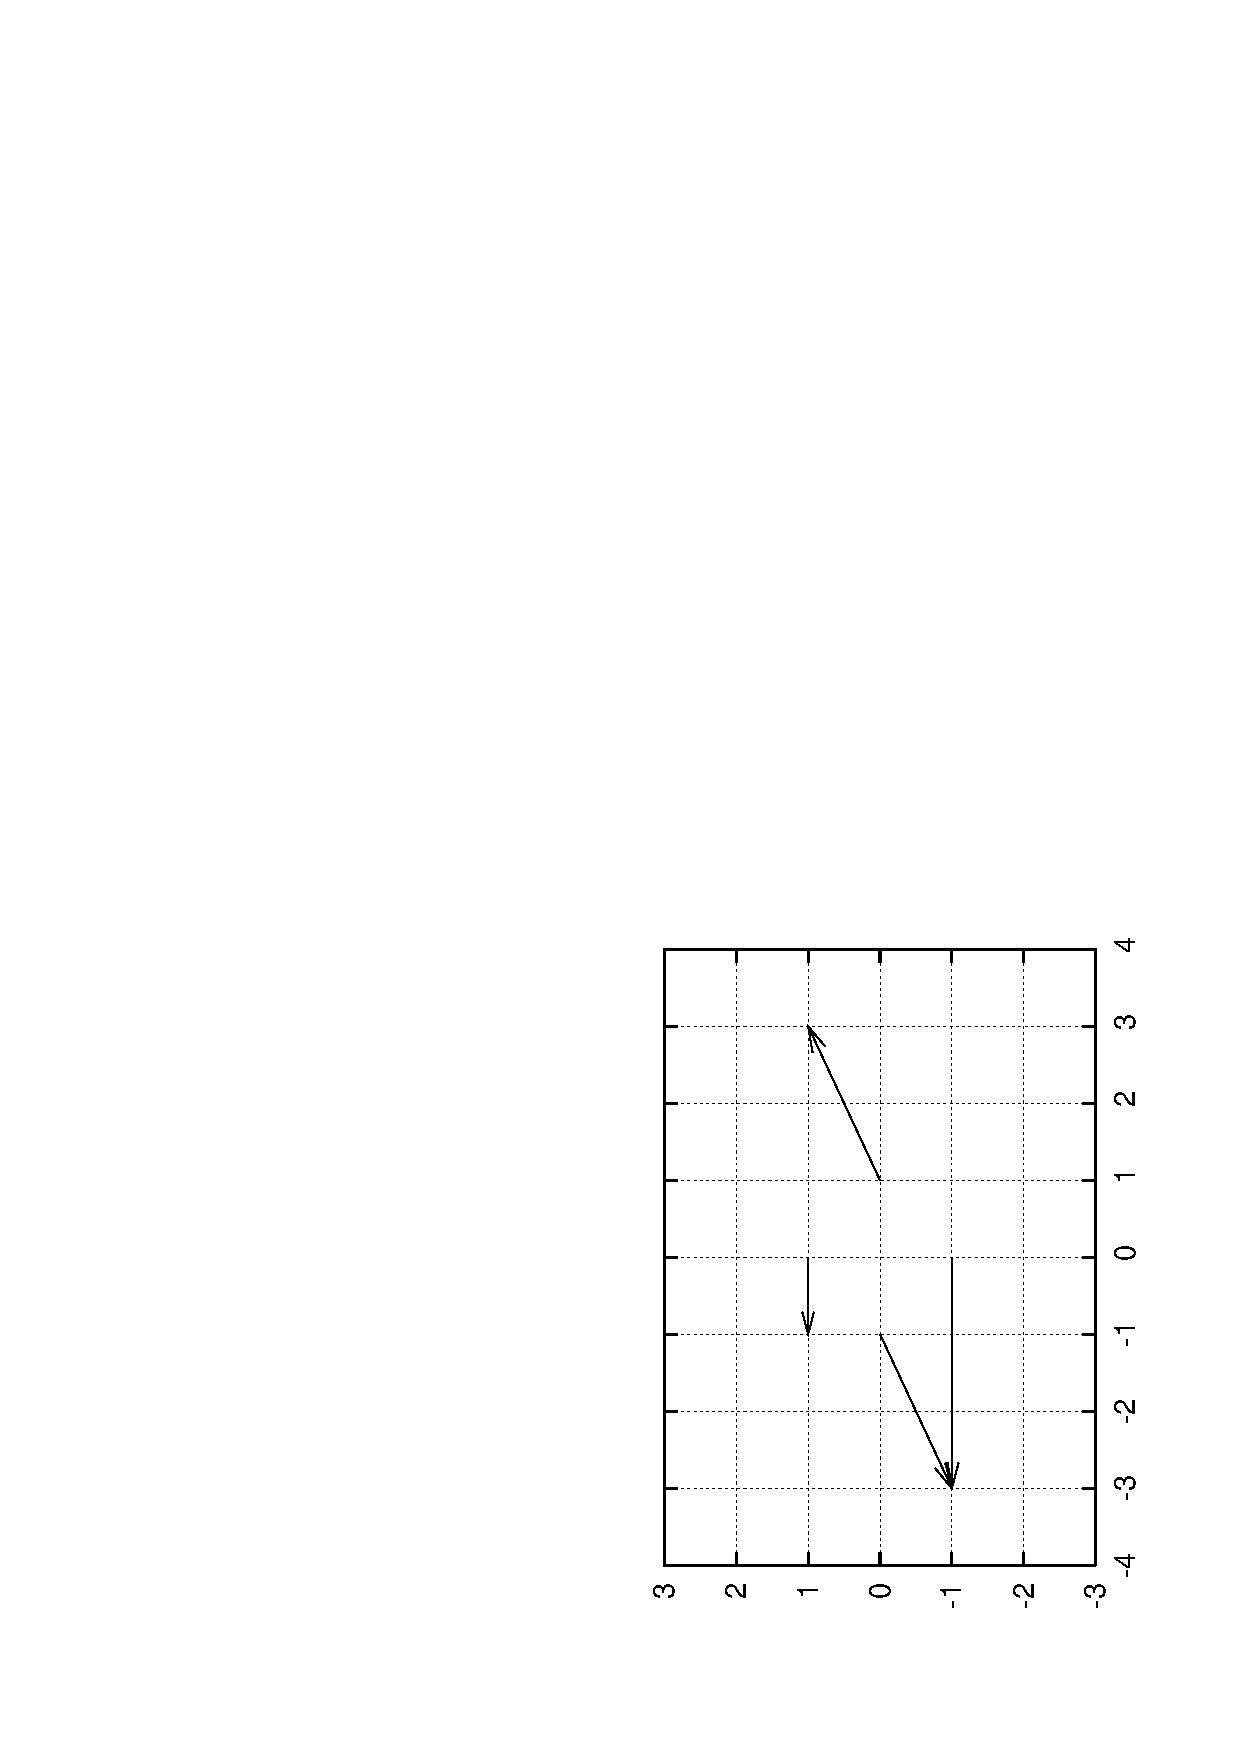
\includegraphics[scale=0.45,angle=270]{img/vectores-par-13}
\end{center}
\end{enumerate}
}
%SOLUCIÓN
{\begin{enumerate}
\item $\nabla f(x,y) = \left(2x-2y^2+\cos(xy)y\, ,\, -4xy+\cos(xy)x\right)$  y
$\nabla g(x,y) = \left((-4x^2-6xy^2+2)\, ,\, (-4xy-6y^3+6y)\right)e^{1-x^2-y^2}$.
\item Los vectores gradientes son de la función $f$.
\end{enumerate}
}
%RESOLUCIÓN
{\begin{enumerate}
\item Para calcular el gradiente necesitamos calcular las derivadas parciales de $f$ y $g$ con respecto a sus variables:
\begin{align*}
\frac{\partial f}{\partial x}(x,y) &= \frac{\partial}{\partial
x}\left(x^2- 2xy^2+\sen(xy)\right)=
2x-2y^2+\cos(xy)\frac{\partial}{\partial x}(xy)=2x-2y^2+\cos(xy)y,\\
\frac{\partial f}{\partial y}(x,y) &= \frac{\partial}{\partial
y}\left(x^2- 2xy^2+\sen(xy)\right)=
-4xy+\cos(xy)\frac{\partial}{\partial y}(xy)=-4xy+\cos(xy)x,\\
\frac{\partial g}{\partial x}(x,y) &= \frac{\partial}{\partial x}\left((2x+3y^2)e^{1-x^2-y^2}\right)=
\frac{\partial}{\partial x}(2x+3y^2)e^{1-x^2-y^2}+(2x+3y^2)\frac{\partial}{\partial x}e^{1-x^2-y^2}=\\
&= 2e^{1-x^2-y^2}+(2x+3y^2)e^{1-x^2-y^2}\frac{\partial}{\partial x}\left(1-x^2-y^2\right) = \\
&= 2e^{1-x^2-y^2}+(2x+3y^2)e^{1-x^2-y^2}(-2x)= (-4x^2-6xy^2+2)e^{1-x^2-y^2},\\
\frac{\partial g}{\partial y}(x,y) &= \frac{\partial}{\partial y}\left((2x+3y^2)e^{1-x^2-y^2}\right)=
\frac{\partial}{\partial x}(2x+3y^2)e^{1-x^2-y^2}+(2x+3y^2)\frac{\partial}{\partial y}e^{1-x^2-y^2}=\\
&= 6y e^{1-x^2-y^2}+(2x+3y^2)e^{1-x^2-y^2}\frac{\partial}{\partial y}\left(1-x^2-y^2\right) =\\
&=6ye^{1-x^2-y^2}+(2x+3y^2)e^{1-x^2-y^2}(-2y)= (-4xy-6y^3+6y)e^{1-x^2-y^2}.
\end{align*}
Así pues, los gradientes son
\begin{align*}
\nabla f(x,y) &=\left(\frac{\partial f}{\partial x}(x,y),\frac{\partial
f}{\partial y}(x,y)\right) = \left(2x-2y^2+\cos(xy)y\, ,\, -4xy+\cos(xy)x\right) \\
\nabla g(x,y) &=\left(\frac{\partial g}{\partial x}(x,y),\frac{\partial
g}{\partial y}(x,y)\right) = \left((-4x^2-6xy^2+2)\, ,\, (-4xy-6y^3+6y)\right)e^{1-x^2-y^2}
\end{align*}

\item Para ver a qué función corresponde la gráfica, calculamos el gradiente en los puntos que nos dan
\begin{align*}
\nabla f(1,0) &= \left(2\cdot 1-2\cdot 0^2+\cos(1\cdot 0)\cdot 0\, ,\, -4\cdot1\cdot0+\cos(1\cdot 0)\cdot1\right) =(2,1),\\
\nabla g(1,0) &= \left((-4\cdot1^2-6\cdot 1\cdot 0^2+2)\, ,\, (-4\cdot 1\cdot 0-6\cdot 0^3+6\cdot 0)\right)e^{1-1^2-0^2}= (-2,0).
\end{align*}
Como el vector libre situado en el punto $(1,0)$ es el $(2,1)$, la gráfica no puede pertenecer a la función $g(x,y)$. Para asegurarnos que se corresponde con la $f(x,y)$, calculamos el gradiente de esta función en el resto de los puntos:
\begin{align*}
\nabla f(0,1) &= \left(2\cdot 0-2\cdot 1^2+\cos(0\cdot 1)\cdot 1\, ,\, -4\cdot0\cdot1+\cos(0\cdot 1)\cdot0\right) =(-1,0),\\
\nabla f(-1,0) &= \left(2\cdot (-1)-2\cdot 0^2+\cos(-1\cdot 0)\cdot 0\, ,\, -4\cdot-1\cdot0+\cos(-1\cdot 0)\cdot(-1)\right) =(-2,-1),\\
\nabla f(0,-1) &= \left(2\cdot 0-2\cdot (-1)^2+\cos(0\cdot (-1))\cdot (-1)\, ,\, -4\cdot0\cdot(-1)+\cos(0\cdot (-1))\cdot0\right) =(-3,0).
\end{align*}
Luego los vectores de la gráfica se corresponden con los vectores gradientes de $f(x,y)$.
\end{enumerate}
}


\newproblem{par-14}{gen}{}
%ENUNCIADO
{Tenemos dos objetos de masas $m_1$ y $m_2$ unidas por una cuerda que pasa a través de una polea como la de la figura.
\begin{center}
  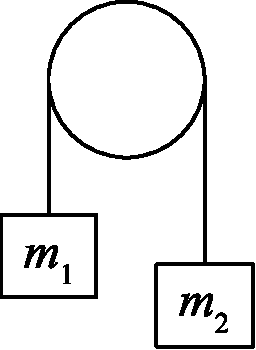
\includegraphics[scale=0.5]{img/polea-par-14}
\end{center}
Si $m_1\geq m_2$, la aceleración de $m_1$ viene dada por la ecuación
\[
a=\frac{m_1-m_2}{m_1+m_2}g,
\]
siendo $g$ la aceleración de la gravedad.
Demostrar que se cumple la ecuación
\[
m_1\frac{\partial a}{\partial m_1}+m_2\frac{\partial a}{\partial m_2}=0.
\]
}
%SOLUCIÓN
{$\dfrac{\partial a}{\partial m_1} = \dfrac{2gm_2}{(m_1+m_2)^2}$ y $\dfrac{\partial a}{\partial m_2} = \dfrac{-2gm_1}{(m_1+m_2)^2}$.
}
%RESOLUCIÓN
{
}


\newproblem{par-15}{gen}{*}
%ENUNCIADO
{La relación que modeliza el potencial eléctrico $V$ de un punto del plano en función de su distancia, es $V=\log D$, donde $D=\sqrt{x^2+y^2}$.

Se pide:
\begin{enumerate}
\item Calcular el gradiente de $V$.
\item Hallar la dirección de máxima variación del potencial
eléctrico en el punto $(x,y)=(\sqrt{3},\sqrt{3})$.
\item Calcular la matriz Hessiana y el Hessiano de $V$ en el punto anterior.
\item Si nos movemos a lo largo de la curva $y=x+1$, cuál será el mínimo potencial alcanzado?
\end{enumerate}
}
%SOLUCIÓN
{\begin{enumerate}
\item $\nabla V(x,y) = \left( \frac{x}{x^2+y^2},\frac{y}{x^2+y^2}\right)$.
\item $\nabla V(\sqrt 3, \sqrt 3) = \sqrt 3 /6(1,1)$.
\item $
HV(x,y) = \left(
\begin{array}{cc}
\frac{y^2-x^2}{y^4+2x^2y^2+x^4} & \frac{-2xy}{y^4+2x^2y^2+x^4} \\
\frac{-2xy}{y^4+2x^2y^2+x^4} & \frac{x^2-y^2}{y^4+2x^2y^2+x^4}
\end{array}
\right),\quad
\left(
\begin{array}{cc}
0 & -1/6 \\
-1/6 & 0
\end{array}
\right),\quad \mbox{y }
|H(\sqrt 3,\sqrt 3)| = -1/36.
$
\item El potencial máximo se alcanza en $(x=-1/2, y=1/2)$ y vale $V(-1/2,1/2) = -\dfrac{\log 2}{2}$.
\end{enumerate}
}
%RESOLUCIÓN
{
}


\newproblem*{par-16}{qui}{}
%ENUNCIADO
{La ecuación unidimensional del calor es
\[
\frac{\partial q}{\partial t}=c^2\frac{\partial^2q}{\partial x^2},
\]
donde $c$ es una constante y $q(x,t)$ es la temperatura de una varilla en un punto que ocupa la posición $x$ en el instante $t$. Demostrar que $q(x,t)=e^{ax+bt}$, con $a\neq 0$, satisface dicha ecuación para un valor apropiado de $c$.
}


\newproblem*{par-17}{amb}{*}
%ENUNCIADO
{Suponiendo que la temperatura, $T$ en ºC, de una zona de la atmósfera es función de la densidad del aire, $d$, en g por cm$^3$, la altura, $h$, en kilómetros, y de la concentración de un determinado elemento, $c$, en mg por cm$^3$, viene dada por la expresión:
\[
T(d,h,c) = \frac{{\ln (dh)}}{c} + c^2 3^{hd}
\]
\begin{enumerate}
\item Suponiendo que la altura a la que medimos la temperatura es de un kilómetro, y que la temperatura medida es de 0 ºC, dar la expresión de la concentración en función de la densidad.
\item Calcular el gradiente de la temperatura en el punto $(d_0,h_0,c_0)=(1,1,2)$.
\item Comprobar que se cumple que:
\[
\frac{{\partial ^2 T}}{{\partial d\partial h}} = \frac{{\partial ^2
T}}{{\partial h\partial d}}
\]
\end{enumerate}
}


\newproblem{par-18}{gen}{}
%ENUNCIADO
{Sea $z(x,y)=\dfrac{x^{2}}{y}+\dfrac{y^{2}}{x}.$ Calcular todas sus derivadas parciales de primer y segundo orden.
}
%SOLUCIÓN
{$\frac{\partial z}{\partial x} = \frac{2x}{y}-\frac{y^2}{x^2}$, $\dfrac{\partial z}{\partial x} = \frac{2y}{x}-\frac{x^2}{y^2}$,\\
$\frac{\partial^2 z}{\partial x^2} = \frac{2y^2}{x^3}+\frac{2}{y}$, $\frac{\partial^2 z}{\partial y\partial x} = -\frac{2y}{x^2}-\frac{2x}{y^2}$, $\frac{\partial^2 z}{\partial x\partial y} = -\frac{2y}{x^2}-\frac{2x}{y^2}$, $\frac{\partial^2 z}{\partial x^2} = \frac{2x^2}{y^3}+\frac{2}{x}$.
}
%RESOLUCIÓN
{
}


\newproblem*{par-19}{gen}{}
%ENUNCIADO
{Dada la función $f(x,y)=\dfrac{x-y}{x+y}$, hallar $\dfrac{\partial f}{\partial x}$ y $\dfrac{\partial f}{\partial y}$ en el punto $(2,-1)$.
}


\newproblem*{par-20}{amb}{*}
%ENUNCIADO
{Supongamos la función de varias variables $f(x,y,z)=x^{3}+\sqrt{xyz}$ que da la presión en un recipiente en función de la posición $(x,y,z)$. Suponiendo que en el recipiente hay un insecto y que se encuentra en el punto de coordenadas $(2,1,3)$, ¿en qué dirección debe moverse si busca ir lo más rápidamente posible hacia zonas de menor presión?
}


\newproblem*{par-21}{gen}{}
%ENUNCIADO
{Dado el siguiente campo escalar expresado en coordenadas cartesianas:
\[
f(x,y,z)=3xy\ln \left( \dfrac{1}{z}\right)
\]
Calcular:
\begin{enumerate}
\item  Su vector gradiente.
\item  Su matriz Hessiana.
\end{enumerate}
}


\newproblem*{par-22}{gen}{*}
%ENUNCIADO
{La definición del polinomio de Taylor de grado 2 de una función de dos variables, $f(x,y)$, centrado en el punto $(x_{0},y_{0})$, es
\begin{align*}
P_{f,(x_0,y_0)}^{2}(x,y)&= f(x_{0},y_{0})+\dfrac{\partial f(x_{0},y_{0})}{\partial x}(x-x_{0})+\dfrac{\partial f(x_{0},y_{0})}{\partial y}(y-y_{0})+\\
&+\dfrac{1}{2}\dfrac{\partial ^{2}f(x_{0},y_{0})}{\partial x^{2}}(x-x_{0})^{2}+\dfrac{1}{2}\dfrac{\partial ^{2}f(x_{0},y_{0})}{\partial y^{2}}(y-y_{0})^{2}+\dfrac{\partial ^{2}f(x_{0},y_{0})}{\partial x\partial y}(x-x_{0})(y-y_{0})
\end{align*}
\begin{enumerate}
\item  Utilizar la fórmula anterior para calcular el polinomio de Taylor de grado 2 de la función $f(x,y)=e^{(x+2y)}$ centrado en $(x_{0},y_{0})=(0,0)$.
\item  Utilizar el polinomio anterior para dar el valor aproximado de $e^{(0.1+2\cdot 0.1)}$.
\end{enumerate}
}


\newproblem*{par-23}{fis}{*}
%ENUNCIADO
{Suponiendo que el potencial eléctrico en un punto de coordenadas cartesianas $(x,y,z)$ viene dado por:
\[
V(x,y,z) = \frac{1} {{x{\kern 1pt} e^y \ln z}},
\]
calcular en el punto $(1,0,e)$:
\begin{enumerate}
\item El campo eléctrico (recordar que el campo eléctrico es el gradiente del potencial cambiado de signo: $\vec E =  - \vec\nabla V$).
\item La divergencia del campo eléctrico.
\end{enumerate}
}


\newproblem*{par-24}{gen}{*}
%ENUNCIADO
{Para la función de 2 variables $f(x,y) = x^{y^2}$
\begin{enumerate}
\item Calcular su dirección y sentido de máximo crecimiento en el punto $(1,1)$.
\item Calcular su matriz Hessiana.
\end{enumerate}
}


\newproblem{par-25}{amb}{*}
%ENUNCIADO
{La Quimiotaxis es el movimiento de los organismos dirigido por un gradiente de concentración, es decir, en la dirección
en la que la concentración aumenta con más rapidez. El moho del cieno Dictyoselium discoideum muestra este
comportamiento. En esta caso, las amebas unicelulares de esta especie se mueven según el gradiente de concentración de
una sustancia química denominada adenosina monofosfato (AMP cíclico). Si suponemos que la expresión que da la
concentración de AMP cíclico en un punto de coordenadas $(x,y,z)$ es:
\[
C(x,y,z) = \frac{4} {{\sqrt {x^2  + y^2  + z^4  + 1} }}
\]
y se sitúa una ameba de moho del cieno en el punto $(-1,0,1)$, ¿en qué dirección se moverá la ameba?
}
%SOLUCIÓN
{$(4/\sqrt{27}, 0, -8/\sqrt{27})$.
}
%RESOLUCIÓN
{
}



%%%%%%% Pendiente 26



\newproblem{par-27}{qui}{*}
%ENUNCIADO
{Supongamos que tenemos una superficie plana, y que la cantidad de una sustancia, $C$ en g/cm$^2$,
depositada sobre cada punto de coordenadas $x$ e $y$, en metros, es función del punto y del tiempo $t$, en horas, y
viene dada por la expresión:
\[
C(x,y,t) = \sqrt{e^{-\frac{3ty}{x^2+1}}}
\]
\begin{enumerate}
\item Calcular la dirección y sentido de máximo crecimiento de la
función en el punto $(x_0,y_0,t_0)=(1,0,1)$.
\item Calcular: $\dfrac{{\partial ^2 C}}{{\partial y\partial x}}$.
\item ¿En qué puntos se anulará el gradiente de $C$?
\end{enumerate}
}
%SOLUCIÓN
{\begin{enumerate}
\item $\nabla C(1,0,1) =\frac{1}{4}(0,-3,0)$.
\item $\displaystyle \frac{\partial^2 C}{\partial y\partial x} =
\frac{e^{-\frac{3ty}{2x^2+2}}}{(2x^2+2)^2}\left(\frac{-36t^2yx}{2x^2+2}+12tx\right)$.
\item En los puntos de la forma $(x,0,0)\ \forall x\in \mathbb{R}$.
\end{enumerate}
}
%RESOLUCIÓN
{Antes de nada conviene simplificar la función:
\[
C(x,y,t) = \sqrt{e^{-\frac{3ty}{x^2+1}}} = \left(e^{-\frac{3ty}{x^2+1}}\right)^{1/2} = e^{-\frac{3ty}{2x^2+2}}
\]
\begin{enumerate}
\item La dirección y sentido de máximo crecimiento de una función de varias variables la da el vector gradiente, en este caso,
\[
\nabla C(x,y,t) =\left(\frac{\partial C}{\partial x}, \frac{\partial C}{\partial y}, \frac{\partial C}{\partial t} \right)
\]
Calulamos las tres derivadas parciales:
\begin{align*}
\frac{\partial C}{\partial x} &= \frac{\partial}{\partial x} e^{-\frac{3ty}{2x^2+2}} = e^{-\frac{3ty}{2x^2+2}} \frac{\partial}{\partial x}\left(-\frac{3ty}{2x^2+2}\right) = e^{-\frac{3ty}{2x^2+2}}\frac{3ty\cdot 4x}{(2x^2+2)^2} \\
\frac{\partial C}{\partial y} &= \frac{\partial}{\partial y} e^{-\frac{3ty}{2x^2+2}} = e^{-\frac{3ty}{2x^2+2}} \frac{\partial}{\partial y}\left(-\frac{3ty}{2x^2+2}\right) = e^{-\frac{3ty}{2x^2+2}}\frac{-3t}{2x^2+2} \\
\frac{\partial C}{\partial t} &= \frac{\partial}{\partial t} e^{-\frac{3ty}{2x^2+2}} = e^{-\frac{3ty}{2x^2+2}} \frac{\partial}{\partial t}\left(-\frac{3ty}{2x^2+2}\right) = e^{-\frac{3ty}{2x^2+2}}\frac{-3y}{2x^2+2}
\end{align*}
De modo que el vector gradiente es
\[
\nabla C(x,y,t) =\frac{e^{-\frac{3ty}{2x^2+2}}}{2x^2+2}\left(\frac{12tyx}{2x^2+2}, -3t, -3y\right),
\]
y en el punto $(x_0,y_0,t_0)=(1,0,1)$ vale
\[
\nabla C(1,0,1) =\frac{e^{-\frac{3\cdot 1\cdot 0}{2\cdot 1^2+2}}}{2\cdot 1^2+2}\left(\frac{12\cdot 1\cdot 0\cdot 1}{2\cdot 1^2+2}, -3\cdot 1, -3\cdot 0\right) = \frac{1}{4}(0,-3,0).
\]

\item
\begin{align*}
\frac{\partial^2 C}{\partial y\partial x} &= \frac{\partial}{\partial y}\frac{\partial C}{\partial x} e^{-\frac{3ty}{2x^2+2}} = \frac{\partial}{\partial y}  \left(e^{-\frac{3ty}{2x^2+2}}\frac{12tyx}{(2x^2+2)^2}\right) = \\
&= \frac{\partial}{\partial y} \left(e^{-\frac{3ty}{2x^2+2}}\right)\frac{12tyx}{(2x^2+2)^2}+e^{-\frac{3ty}{2x^2+2}}\frac{\partial}{\partial y}\left(\frac{12tyx}{(2x^2+2)^2}\right) = \\
&= e^{-\frac{3ty}{2x^2+2}}\frac{\partial}{\partial y}\left(-\frac{3ty}{2x^2+2}\right)\frac{3ty\cdot 4x}{(2x^2+2)^2}+e^{-\frac{3ty}{2x^2+2}}\frac{12tx}{(2x^2+2)^2} = \\
&= e^{-\frac{3ty}{2x^2+2}}\frac{-3t}{2x^2+2}\frac{3ty\cdot 4x}{(2x^2+2)^2}+e^{-\frac{3ty}{2x^2+2}}\frac{12tx}{(2x^2+2)^2} = \\
&= \frac{e^{-\frac{3ty}{2x^2+2}}}{(2x^2+2)^2}\left(\frac{-36t^2yx}{2x^2+2}+12tx\right).
\end{align*}

\item
\[
\nabla C(x,y,t) =\frac{e^{-\frac{3ty}{2x^2+2}}}{2x^2+2}\left(\frac{12tyx}{2x^2+2}, -3t, -3y\right) = (0,0,0) \Leftrightarrow
\left\{
\begin{array}{l}
12txy =0 \\
-3t = 0\\
-3y = 0
\end{array}
\right.
\]
de donde se deduce que $t=0$, $y=0$ y $x$ puede tomar cualquier valor. Así pues, los puntos que anulan el gradiente son de la forma $(x,0,0)$, $x\in\mathbb{R}$.
\end{enumerate}
}


\newproblem{par-28}{fis}{*}
%ENUNCIADO
{Una barra de metal de un metro de largo se calienta de manera irregular y de forma tal que a $x$ metros de su extremo izquierdo y en el instante $t$ minutos, su temperatura en grados centígrados esta dada por $H(x,t) = 100e^{-0.1t}\sen(\pi xt)$ con $0\leq x \leq 1$.
\begin{enumerate}
\item Calcular $\dfrac{\partial H}{\partial x}(0.2, 1)$ y $\dfrac{\partial H}{\partial x}(0.8, 1).$ ¿Cuál es la interpretación práctica (en términos de temperatura) de estas derivadas parciales? Explicar por qué cada una tiene el signo que tiene.
\item Calcular la matriz hessiana de $H$.
\end{enumerate}
}
%SOLUCIÓN
{\begin{enumerate}
\item $\frac{\partial H}{\partial x}(0.2,\, 1) = 100e^{-0.1}\cos(0.2\pi) \pi = 229.9736$ \\
$\frac{\partial H}{\partial x}(0.8,\, 1) = 100e^{-0.1}\cos(0.8\pi) \pi = -229.9736$.
\item $
\left(
\begin{array}{cc}
-100e^{-0.1t}\pi^2 t^2\sen(\pi xt) & 100e^{-0.1t}\left((-0.1\pi t+\pi)\cos(\pi xt) - \pi^2 xt \sen(\pi xt)\right) \\
100e^{-0.1t}\left((-0.1\pi t+\pi)\cos(\pi xt) - \pi^2 xt \sen(\pi xt)\right) & 100e^{-0.1t}\left(0.01\sen(\pi xt) -(0.2+\pi^2x^2) \cos(\pi xt)\right)
\end{array}
\right)$
\end{enumerate}
}
%RESOLUCIÓN
{\begin{enumerate}
\item La derivada parcial de $H$ con respecto a $x$ es
\begin{align*}
\frac{\partial H}{\partial x}(x,t) &= 100e^{-0.1t}\cos(\pi xt) \pi t \\
\end{align*}
y en los puntos que nos piden vale
\begin{align*}
\frac{\partial H}{\partial x}(0.2,\, 1) &= 100e^{-0.1}\cos(0.2\pi) \pi =
229.9736\\
\frac{\partial H}{\partial x}(0.8,\, 1) &= 100e^{-0.1}\cos(0.8\pi) \pi =
-229.9736
\end{align*}
La derivada parcial $\dfrac{\partial H}{\partial x}(x_0,t_0)$ indica la variación instantánea que experimenta la temperatura con respecto a la variación de la distancia al extremo izquierdo en el punto. El signo de la derviada parcial indica si la variación de la temperatura es creciente (aumenta la temperatura) o decreciente (disminuye). Así en el punto $(0.2,\, 1)$ la temperatura aumentará a razón de $229.9736$ grados centígrados por cada metro que nos alejemos del extremo izquierdo de la barra de metal, mientras que en el $(0.8,\,1)$ la temperatura disminuirá a razón de $229.9736$ grados centígrados por cada metro que nos alejemos del extremo izquierdo de la barra de metal.

\item Para calcular la matriz Hessiana necesitamos las derivadas parciales de
segundo orden:
\begin{align*}
\frac{\partial H}{\partial t} (x,t) &= 100\left(\frac{\partial}{\partial x} e^{-0.1 t} \sen (\pi xt) + e^{-0.1t}\frac{\partial}{\partial x}\sen(\pi xt)\right)=\\
&= 100\left(-0.1e^{-0.1t}\sen(\pi xt) +e^{-0.1t}\cos(\pi xt)\pi x\right) =\\
&= 100 e^{-0.1t}\left(-0.1 \sen(\pi xt) + \pi x \cos(\pi xt)\right),\\
\frac{\partial^2 H}{\partial x^2}(x,t) &= \frac{\partial}{\partial x}\left(100e^{-0.1t}\pi t\cos(\pi xt) \right) = 100e^{-0.1t}\pi t(-\sen(\pi xt) \pi t) =\\
&= -100e^{-0.1t}\pi^2 t^2\sen(\pi xt),\\
\frac{\partial^2 H}{\partial t\partial x}(x,t) &= \frac{\partial}{\partial t}\left(100e^{-0.1t}\pi t\cos(\pi xt) \right) =\\
&= 100\left(\frac{\partial}{\partial t}e^{-0.1t}\pi t\cos(\pi xt) + e^{-0.1t}\left(\frac{\partial}{\partial t}(\pi t)\cos(\pi xt) + \pi t \frac{\partial}{\partial t}\cos(\pi xt)\right) \right) =\\
&= 100\left(-0.1e^{-0.1t}\pi t\cos(\pi xt) + e^{-0.1t}\left(\pi \cos(\pi xt) - \pi t \sen(\pi xt)\pi x\right) \right) =\\
&= 100e^{-0.1t}\left(-0.1\pi t\cos(\pi xt)+\pi \cos(\pi xt) - \pi^2 xt \sen(\pi xt)\right) = \\
&= 100e^{-0.1t}\left((-0.1\pi t+\pi)\cos(\pi xt) - \pi^2 xt \sen(\pi xt)\right),\\
\end{align*}

\begin{align*}
\frac{\partial^2 H}{\partial x\partial t}(x,t) &= \frac{\partial^2 H}{\partial t\partial x}(x,t) \quad (\mbox{igualdad de las derivadas cruzadas por el teorema de Schwartz})\\
\frac{\partial^2 H}{\partial t^2}(x,t) &= \frac{\partial}{\partial t} \left(100 e^{-0.1t}\left(-0.1 \sen(\pi xt) + \pi x \cos(\pi xt)\right)\right)  =\\
&= 100\left(\frac{\partial}{\partial t} e^{-0.1t}\left(-0.1 \sen(\pi xt) + \pi x \cos(\pi xt)\right) +\right.\\
&\left. \qquad + e^{0.1t}\left(\frac{\partial}{\partial t}\left(-0.1\sen(\pi xt)\right) + \frac{\partial}{\partial t}\left(\pi x \cos(\pi xt)\right)\right)\right) =\\
&= 100\left(-0.1 e^{-0.1t}\left(-0.1 \sen(\pi xt) + \pi x \cos(\pi xt)\right)\right. +\\
&\left. \qquad + e^{0.1t}\left(-0.1\cos(\pi xt)\pi x - \pi x \cos(\pi xt)\pi x\right)\right) =\\
&= 100e^{-0.1t}\left(0.01\sen(\pi xt) -0.1 \pi x \cos(\pi xt) -0.1\pi x\cos(\pi xt) - \pi^2 x^2 \cos(\pi xt)\right) = \\
&= 100e^{-0.1t}\left(0.01\sen(\pi xt) -(0.2+\pi^2x^2) \cos(\pi xt)\right).
\end{align*}
Así pues, la matriz Hessiana es
\[
\left(
\begin{array}{cc}
-100e^{-0.1t}\pi^2 t^2\sen(\pi xt) & 100e^{-0.1t}\left((-0.1\pi t+\pi)\cos(\pi xt) - \pi^2 xt \sen(\pi xt)\right) \\
100e^{-0.1t}\left((-0.1\pi t+\pi)\cos(\pi xt) - \pi^2 xt \sen(\pi xt)\right) & 100e^{-0.1t}\left(0.01\sen(\pi xt) -(0.2+\pi^2x^2) \cos(\pi xt)\right)
\end{array}
\right)
\]
\end{enumerate}
}


\newproblem{par-29}{gen}{*}
%ENUNCIADO
{Dar la dirección de máximo crecimiento de la función
\[
f(x,y,z) = \frac{\log(zx)}z-xe^{-zxy}
\]
en el punto $(1,1,1)$.
}
%SOLUCIÓN
{$\nabla f(1,1,1)=(1,e^{-1},1+e^{-1})$.
}
%RESOLUCIÓN
{La dirección de máximo crecimiento de una función de varias variables la da el vector gradiente:
\[
\nabla f(x,y,z) = \left(\frac{\partial f}{\partial x}(x,y,z),\frac{\partial f}{\partial y}(x,y,z),\frac{\partial f}{\partial z}(x,y,z)\right)
\]
Calculamos por tanto cada una de las derivadas parciales que aparecen en las componentes del vector:
\begin{align*}
\frac{\partial f}{\partial x}(x,y,z) &= \frac{\partial}{\partial x}(\frac{\log (zx)}z-xe^{-zxy}) = \frac{\partial}{\partial x}(\frac{\log (zx)}z)-\frac{\partial}{\partial x}(xe^{-zxy})= \\
&= \frac{1}{z}\frac{\partial}{\partial x}(\log (zx))-(\frac{\partial}{\partial x}(x)e^{-zxy}+x\frac{\partial}{\partial x}(e^{-zxy}))= \\
&= \frac{1}{z}\frac{1}{zx}\frac{\partial}{\partial x}(zx)-(e^{-zxy}+xe^{-zxy}\frac{\partial}{\partial x}(-zxy))= \\
&= \frac{1}{z}\frac{1}{zx}z-(e^{-zxy}+xe^{-zxy}(-zy)) = \frac{1}{zx}-e^{-zxy}(1-xyz),\\
\frac{\partial f}{\partial y}(x,y,z) &= \frac{\partial}{\partial y}(\frac{\log(zx)}z-xe^{-zxy}) = \frac{\partial}{\partial y}(\frac{\log (zx)}z)-\frac{\partial}{\partial y}(xe^{-zxy})= \\
&= -x\frac{\partial}{\partial y}(e^{-zxy}) = -xe^{-zxy}\frac{\partial}{\partial y}(-zxy)=x^2ze^{-zxy},\\
\frac{\partial f}{\partial z}(x,y,z) &= \frac{\partial}{\partial z}(\frac{\log(zx)}z-xe^{-zxy}) = \frac{\partial}{\partial z}(\frac{\log (zx)}z)-\frac{\partial}{\partial z}(xe^{-zxy})= \\
&= \frac{\frac{\partial}{\partial z}(\log (zx))z-\log (zx)\frac{\partial}{\partial z}(z)}{z^2}-x\frac{\partial}{\partial z}(e^{-zxy}))= \\
&= \frac{\frac 1{zx}\frac \partial {\partial z}(zx)z-\log (zx)}{z^2}-xe^{-zxy}\frac{\partial}{\partial z}(-zxy))= \\
&= \frac{\frac 1{zx}xz-\log (zx)}{z^2}-xe^{-zxy}-xy=\frac{1-\log (zx)}{z^2}+x^2ye^{-zxy}.
\end{align*}
Por lo tanto, el vector gradiente será:
\[
\nabla f(x,y,z)=(\frac{1}{zx}-e^{-zxy}(1-xyz), x^2ze^{-zxy}, \frac{1-\log (zx)}{z^2}+x^2ye^{-zxy})
\]

Finalmente, como nos pieden la dirección de máximo crecimiento en el punto $(1,1,1)$, tendremos que particularizar el vector gradiente en dicho punto, es decir:
\[
\nabla f(1,1,1)=(1,e^{-1},1+e^{-1}).
\]
}


\newproblem{par-30}{gen}{*}
%ENUNCIADO
{Calcular el gradiente de la función
\[
f(x,y,z)=e^{\sqrt{x^2+2yz}}+\ln (\frac{xy}z)
\]
en el punto $(1,-2,-2)$.
}
%SOLUCIÓN
{$\nabla f(x,y,z)=\left(\frac{xe^{\sqrt{x^2+2yz}}}{\sqrt{x^2+2yz}}+\frac{1}{x}, \frac{ze^{\sqrt{x^2+2yz}}}{\sqrt{x^2+2yz}}+\frac{1}{y}, \frac{ye^{\sqrt{x^2+2yz}}}{\sqrt{x^2+2yz}}-\frac{1}{z}\right)$\\ y $\nabla f(1,-2,-2)=\left(\frac{e^3}{3}+1,\frac{-2e^3}{3}-\frac{1}{2},\frac{-2e^3}{3}+\frac{1}{2}\right)$.}
%RESOLUCIÓN
{El gradiente de $f(x,y,z)$ se define como el vector $\nabla f(x,y,z)=\left(\dfrac{\partial f}{\partial x}(x,y,z),\dfrac{\partial f}{\partial y}(x,y,z),\dfrac{\partial f}{\partial z}(x,y,z)\right).$ Por tanto, tenemos que calcular las tres derivadas parciales siguientes:
\begin{align*}
\dfrac{\partial f}{\partial x}(x,y,z) &= \dfrac{\partial}{\partial x}(e^{\sqrt{x^2+2yz}}+\ln (\frac{xy}z)) = \dfrac{\partial}{\partial x}(e^{\sqrt{x^2+2yz}})+\dfrac{\partial}{\partial x}(\ln (\frac{xy}z))= \\
&= e^{\sqrt{x^2+2yz}}\dfrac \partial {\partial x}(\sqrt{x^2+2yz})+\frac{1}{xy/z}\dfrac{\partial}{\partial x}(\frac{xy}z)= \\
&= e^{\sqrt{x^2+2yz}}\frac{1}{2\sqrt{x^2+2yz}}\dfrac{\partial}{\partial x}(x^2+2yz)+\frac{z}{xy}\frac{y}{z}= \\
&= e^{\sqrt{x^2+2yz}}\frac{1}{2\sqrt{x^2+2yz}}2x+\frac{1}{x} = \frac{xe^{\sqrt{x^2+2yz}}}{\sqrt{x^2+2yz}}+\frac{1}{x}, \\
\dfrac{\partial f}{\partial y}(x,y,z) &= \dfrac{\partial}{\partial y}(e^{\sqrt{x^2+2yz}}+\ln (\frac{xy}z)) = \dfrac{\partial}{\partial y}(e^{\sqrt{x^2+2yz}})+\dfrac{\partial}{\partial y}(\ln (\frac{xy}z))= \\
&= e^{\sqrt{x^2+2yz}}\dfrac{\partial}{\partial y}(\sqrt{x^2+2yz})+\frac{1}{xy/z}\dfrac{\partial}{\partial y}(\frac{xy}z)= \\
&= e^{\sqrt{x^2+2yz}}\frac{1}{2\sqrt{x^2+2yz}}\dfrac{\partial}{\partial y}(x^2+2yz)+\frac{z}{xy}\frac{x}{z}= \\
&= e^{\sqrt{x^2+2yz}}\frac{1}{2\sqrt{x^2+2yz}}2z+\frac{1}{y}=\frac{ze^{\sqrt{x^2+2yz}}}{\sqrt{x^2+2yz}}+\frac{1}{y}, \\
\dfrac{\partial f}{\partial z}(x,y,z) &= \dfrac{\partial}{\partial z}(e^{\sqrt{x^2+2yz}}+\ln (\frac{xy}z)) = \dfrac{\partial}{\partial z}(e^{\sqrt{x^2+2yz}})+\dfrac{\partial}{\partial z}(\ln (\frac{xy}{z}))= \\
&= e^{\sqrt{x^2+2yz}}\dfrac{\partial}{\partial z}(\sqrt{x^2+2yz})+\frac{1}{xy/z}\dfrac{\partial}{\partial z}(\frac{xy}{z})= \\
&= e^{\sqrt{x^2+2yz}}\frac{1}{2\sqrt{x^2+2yz}}\dfrac{\partial}{\partial z}(x^2+2yz)+\frac{z}{xy}\frac{-xy}{z^2}= \\
&= e^{\sqrt{x^2+2yz}}\frac{1}{2\sqrt{x^2+2yz}}2y-\frac{1}{z} = \frac{ye^{\sqrt{x^2+2yz}}}{\sqrt{x^2+2yz}}-\frac{1}{z},
\end{align*}
y, en consecuencia tenemos
\[
\nabla f(x,y,z)=\left(\frac{xe^{\sqrt{x^2+2yz}}}{\sqrt{x^2+2yz}}+\frac{1}{x}, \frac{ze^{\sqrt{x^2+2yz}}}{\sqrt{x^2+2yz}}+\frac{1}{y}, \frac{ye^{\sqrt{x^2+2yz}}}{\sqrt{x^2+2yz}}-\frac{1}{z}\right).
\]
Como nos piden el gradiente en el punto $(1,-2,-2),$ sustituimos $x$ por 1, $y$ por -2, y $z$ por -2 en el vector anterior y obtenemos
\[
\nabla f(1,-2,-2)=\left(\frac{e^3}{3}+1,\frac{-2e^3}{3}-\frac{1}{2},\frac{-2e^3}{3}+\frac{1}{2}\right).
\]
}


\newproblem{par-31}{gen}{*}
%ENUNCIADO
{Calcular el vector gradiente de la función
\[
\log \left( \sqrt{x^{2}-z^{2}}\right) +3^{\tfrac{x^{2}}{y}}
\]
en el punto $(1,1,0)$.
}
%SOLUCIÓN
{$\nabla f(x,y,z)=(\frac{x}{x^{2}-z^{2}}+3^{\tfrac{x^{2}}{y}}\log 3\dfrac{2x}{y},3^{\tfrac{x^{2}}{y}}\log 3\dfrac{-x^{2}}{y^{2}},-\frac{z}{x^{2}-z^{2}})$, y $\nabla f(1,-2,-2)=(1+6\log 3,-3\log 3,0)$.
}
%RESOLUCIÓN
{El gradiente de $f(x,y,z)$ se define como el vector $\nabla f(x,y,z)=(\dfrac{\partial f}{\partial x}(x,y,z),\dfrac{\partial f}{\partial y}(x,y,z),\dfrac{\partial f}{\partial z}(x,y,z))$. Por tanto, tenemos que calcular las tres derivadas parciales siguientes:
\begin{align*}
\dfrac{\partial f}{\partial x}(x,y,z) &= \dfrac{\partial }{\partial x}(\log\left(\sqrt{x^{2}-z^{2}}\right) +3^{\tfrac{x^{2}}{y}}) = \dfrac{\partial }{\partial x}(\log \left(\sqrt{x^{2}-z^{2}}\right) )+\dfrac{\partial }{\partial x}(3^{\tfrac{x^{2}}{y}})= \\
&= \frac{1}{\sqrt{x^{2}-z^{2}}}\dfrac{\partial }{\partial x}(\sqrt{x^{2}-z^{2}})+3^{\tfrac{x^{2}}{y}}\log 3\dfrac{\partial }{\partial x}(\dfrac{x^{2}}{y}) = \\
&= \frac{1}{\sqrt{x^{2}-z^{2}}}\frac{1}{2\sqrt{x^{2}-z^{2}}}\dfrac{\partial}{\partial x}(x^{2}-z^{2})+3^{\tfrac{x^{2}}{y}}\log 3\dfrac{2x}{y}= \\
&= \frac{1}{2(x^{2}-z^{2})}2x+3^{\tfrac{x^{2}}{y}}\log 3\dfrac{2x}{y}=\frac{x}{x^{2}-z^{2}}+3^{\tfrac{x^{2}}{y}}\log 3\dfrac{2x}{y}, \\
\dfrac{\partial f}{\partial y}(x,y,z) &= \dfrac{\partial }{\partial y}(\log\left( \sqrt{x^{2}-z^{2}}\right) +3^{\tfrac{x^{2}}{y}}) = \dfrac{\partial }{\partial y}(\log \left( \sqrt{x^{2}-z^{2}}\right) )+\dfrac{\partial }{\partial y}(3^{\tfrac{x^{2}}{y}})= \\
&= 0+3^{\tfrac{x^{2}}{y}}\log 3\dfrac{\partial }{\partial y}(\dfrac{x^{2}}{y}) = 3^{\tfrac{x^{2}}{y}}\log 3\dfrac{-x^{2}}{y^{2}}, \\
\dfrac{\partial f}{\partial z}(x,y,z) &= \dfrac{\partial }{\partial z}(\log\left( \sqrt{x^{2}-z^{2}}\right) +3^{\tfrac{x^{2}}{y}}) = \dfrac{\partial }{\partial z}(\log \left( \sqrt{x^{2}-z^{2}}\right) )+\dfrac{\partial }{\partial z}(3^{\tfrac{x^{2}}{y}})= \\
&= \frac{1}{\sqrt{x^{2}-z^{2}}}\dfrac{\partial }{\partial x}(\sqrt{x^{2}-z^{2}})+0 = \frac{1}{\sqrt{x^{2}-z^{2}}}\frac{1}{2\sqrt{x^{2}-z^{2}}}\dfrac{\partial }{\partial x}(x^{2}-z^{2})= \\
&= \frac{1}{2(x^{2}-z^{2})}(-2z)=-\frac{z}{x^{2}-z^{2}}.
\end{align*}
y, en consecuencia tenemos
\[
\nabla f(x,y,z)=(\frac{x}{x^{2}-z^{2}}+3^{\tfrac{x^{2}}{y}}\log 3\dfrac{2x}{y},3^{\tfrac{x^{2}}{y}}\log 3\dfrac{-x^{2}}{y^{2}},-\frac{z}{x^{2}-z^{2}}).
\]
Como nos piden el gradiente en el punto $(1,1,0),$ sustituimos $x$ por 1, $y$
por 1, y $z$ por 0 en el vector anterior y obtenemos
\[
\nabla f(1,-2,-2)=(1+6\log 3,-3\log 3,0).
\]
}


\newproblem{par-32}{amb}{}
%ENUNCIADO
{La asimilación de CO$_2$ de una planta depende de la temperatura ambiente (t) y de la intensidad de la luz (l), según la función
\[
f(t,l) = ctl^2,
\]
donde $c$ es una constante.
Estudiar cómo evoluciona la asimilación de CO$_2$ para distintas intensidades de luz, cuando se mantiene la temperatura constante.
Estudiar también cómo evoluciona para distintas temperaturas cuando se mantiene la intensidad de la luz constante.
}
%SOLUCIÓN
{$\frac{\partial f}{\partial l}(t,l) = 2ctl$ y $\frac{\partial f}{\partial t}(t,l) = cl^2$.
}
%RESOLUCIÓN
{
}


\newproblem{par-33}{amb}{}
%ENUNCIADO
{La abundancia de una determinada especie de planta depende del nivel de nitrógeno en el suelo y del nivel de perturbaciones, de manera que un incremento del nivel de nitrógeno tiene un efecto negativo en la abundancia de esta especie, y un aumento de las perturbaciones también tiene un efecto negativo.
Si en un momento dado comienza a aumentar el nivel de nitrógeno en el suelo y también las perturbaciones debidas al pastoreo, ¿cómo se verá afectada la abundancia de la especie?
}
%SOLUCIÓN
{La abundancia de la especie disminuirá.
}
%RESOLUCIÓN
{
}


\newproblem{par-34}{amb}{}
%ENUNCIADO
{La velocidad de crecimiento de un organismo depende de la disponibilidad de alimento y del número de competidores en busca de alimento.
¿Cómo se verá afectada la velocidad de crecimiento si la disponibilidad de alimento aumenta con el tiempo y el número de competidores disminuye?}
%SOLUCIÓN
{La velocidad de crecimiento aumentará.
}
%RESOLUCIÓN
{
}


\newproblem{par-35}{amb}{}
%ENUNCIADO
{Un organismo se mueve sobre una superficie inclinada siguiendo la línea de máxima pendiente descendiente.
Si la expresión de la superficie es
\[
f(x,y) = x^2-y^2,
\]
calcule la dirección en la que se moverá el organismo en el punto $(2,3)$.
}
%SOLUCIÓN
{Se moverá en la dirección $-\nabla f(2,3)=(-4,6)$.}
%RESOLUCIÓN
{
}


\newproblem{par-36}{gen}{}
%ENUNCIADO
{Si $f(x,y,z)=x^3y^2z$ y $g(t)=(e^t,\cos t,\sen t)$, calcular $(f\circ g)'(t)$.
}
%SOLUCIÓN
{$(f\circ g)'(t)= e^{3t}(3\sen t\cos^2 t-2\sen^2 t\cos t+\cos^3 t)$.
}
%RESOLUCIÓN
{
}


\newproblem{par-37}{amb}{}
%ENUNCIADO
{Obtener los puntos críticos de $z=f(x,y)$ para:
\begin{enumerate}
\item $f(x,y)=x^2+y^2$.
\item $f(x,y)=x^2y+y^2x$.
\item $f(x,y)=x^2-2xy+2y^2$.
\end{enumerate}
}
%SOLUCIÓN
{\begin{enumerate}
\item $(0,0)$.
\item $(0,0)$.
\item $(0,0)$.
\end{enumerate}
}
%RESOLUCIÓN
{
}


\newproblem{par-38}{gen}{}
%ENUNCIADO
{La superficie de una montaña tiene la forma
\[
S:z=a-bx^2-cy^2,
\]
donde $a$, $b$ y $c$ son constantes, $x$ es la coordenada Este-Oeste e $y$ la coordenada Norte-Sur en el mapa, y $z$ la altura sobre el nivel del mar en metros.
En el punto $P=(1,1)$ del mapa, ¿en qué dirección crece más rápidamente la altura?
}
%SOLUCIÓN
{$(-2b,-2c)$.
}
%RESOLUCIÓN
{
}


\newproblem{par-39}{gen}{}
%ENUNCIADO
{Hallar las direcciones de máximo y mínimo crecimiento de las siguientes funciones en el punto $P$:
\begin{enumerate}
\item $f(x,y)=x^2+xy+y^2$, $P=(-1,1)$.
\item $f(x,y)=x^2y+e^{xy}\sen y$, $P=(1,0)$.
\item $f(x,y,z)=\log(xy)+\log(yz)+\log(xz)$, $P=(1,1,1)$.
\item $f(x,y,z)=\log(x^2+y^2-1)+y+6z$, $P=(1,1,0)$.
\end{enumerate}
}
%SOLUCIÓN
{\begin{enumerate}
\item Máximo crecimiento en la dirección $(-1,1)$ y máximo decrecimiento en la dirección $(1,-1)$.
\item Máximo crecimiento en la dirección $(0,2)$ y máximo decrecimiento en la dirección $(0,-2)$.
\item Máximo crecimiento en la dirección $(2,2,2)$ y máximo decrecimiento en la dirección $(-2,-2,-2)$.
\item Máximo crecimiento en la dirección $(2,3,6)$ y máximo decrecimiento en la dirección $(-2,-3,-6)$.
\end{enumerate}
}
%RESOLUCIÓN
{
}


\newproblem{par-40}{gen}{}
%ENUNCIADO
{¿En qué direcciones se anulará la derivada direccional de la función
\[
f(x,y)=\frac{x^2-y^2}{x^2+y^2}
\]
en el punto $P=(1,1)$?
}
%SOLUCIÓN
{En la dirección $(1/\sqrt{2},1/\sqrt{2})$.
}
%RESOLUCIÓN
{
}


\newproblem{par-41}{gen}{}
%ENUNCIADO
{¿Existe alguna dirección en la que la derivada direccional en el punto $P=(1,2)$ de la función
\[
f(x,y) = x^2-3xy+4y^2
\]
valga 14?
}
%SOLUCIÓN
{No.
}
%RESOLUCIÓN
{
}


\newproblem{par-42}{gen}{}
%ENUNCIADO
{La derivada direccional de una función $f$ en un punto $P$ es máxima en la dirección del vector $(1,1,-1)$ y su valor es $2\sqrt{3}$.
¿Cuánto vale la derivada direccional de $f$ en $P$ en la dirección del vector $(1,1,0)$?
}
%SOLUCIÓN
{$2\sqrt{2}$.
}
%RESOLUCIÓN
{
}


\newproblem{par-43}{gen}{}
%ENUNCIADO
{Dado el campo escalar
\[
f(x,y,z) = x^2-y^2+xyz^3-zx
\]
en el punto $P=(1,2,3)$, se pide:
\begin{enumerate}
\item Calcular la derivada direccional de $f$ en $P$ a lo largo del vector unitario $\mathbf{u}=\frac{1}{\sqrt2}(1,-1,0)$.
\item ¿En qué dirección es máxima la derivada direccional de $f$ en $P$? Obtener el valor de dicha derivada direccional.
\end{enumerate}
}
%SOLUCIÓN
{\begin{enumerate}
\item $15\sqrt{2}$.
\item La derivada direccional es máxima en la dirección del gradiente $(53,23,53)$ y vale $\sqrt{6147}$.
\end{enumerate}
}
%RESOLUCIÓN
{
}


\newproblem*{par-44}{gen}{}
%ENUNCIADO
{En el ajuste de regresión de una recta $y=a+bx$, se suele utilizar la técnica de mínimos cuadrados que consisten en buscar los valores
de $a$ y $b$ que hacen mínima la función
\[
f(a,b)= \sum_{i=1}^{n}(y_i-a-bx_i)^2,
\]
donde el sumatorio abarca a todos los pares de la muestra $(x_i,y_i)$ para $i=1,\ldots, n$, siendo $n$ el tamaño de la muestra.

Demostrar que esta función alcanza el mínimo en los puntos
\[
a=\bar y-b\bar x \quad \mbox{ y } b=\frac{s_{xy}}{s_x^2}.
\]
}
%SOLUCIÓN
{
}
%RESOLUCIÓN
{
}


\newproblem*{par-45}{gen}{}
%STATEMENT
{La siguiente función mide la presión del aire en la posición $(x,y,z)$.
\[
f(x,y,z)= x^2+y^2-z^3.
\]
Sea $A$ un objeto que se mueve a lo largo de la trayectoria:
\[
\begin{cases}
x=t\\
y=1\\
z=1/t
\end{cases}
t>0.
\]
\begin{enumerate}
\item Calcular la ecuación de la recta tangente a la trayectoria de $A$ en el punto $(1,1,1)$.
\item Sigue la trayectoria de $A$ en el punto $(1,1,1)$ la dirección de máximo crecimiento de la función $f$?
\end{enumerate}
}
%SOLUTION
{\begin{enumerate}
\item $(1+t, 1, 1-t)$.
\item No ya que la dirección de máximo crecimiento de $f$ es $\nabla f(1,1,1)=(2,2,-3)$ y la dirección de la trayectoria es $(1,0,-1)$.
\end{enumerate}
}
%RESOLUTION
{
}


\newproblem{par-46}{gen}{*}
%STATEMENT
{Obtener la ecuación del plano tangente y de la recta normal a la superficie
\[
S:xyz=8
\]
en el punto $P=(4,-2,-1)$.
}
%SOLUTION
{Recta normal $l:(4+2t,-2-4t,-1-8t)$. Plano tangente $\pi: 2x-4y-8z+24=0$.
}
%RESOLUTION
{
}


%%%%%%% Pendiente 26

% Autor: Alfredo Sánchez Alberca (asalber@ceu.es)

\newproblem{dersup-1}{gen}{*}
%ENUNCIADO
{Obtener la ecuación del plano tangente y de la recta normal a la superficie 
\[
S:xyz=8
\]
en el punto $P=(4,-2,-1)$.
}
%SOLUCIÓN
{Recta normal $l:(4+2t,-2-4t,-1-8t)$. Plano tangente $\pi: 2x-4y-8z+24=0$. 
}
%RESOLUCIÓN
{
}

% Autor: Alfredo Sánchez Alberca (asalber@ceu.es)

\newproblem{derimpn-1}{gen}{}
%ENUNCIADO
{Suponiendo que $z$ es función de $x$ e $y$ ($z=f(x,y)$), a partir de la ecuación $F(x,y,z)=0$, deducir que 
\[
\frac{\partial z}{\partial x} = \frac{-\dfrac{\partial F}{\partial x}}{\dfrac{\partial F}{\partial z}}
\quad \mbox{y} \quad
\frac{\partial z}{\partial y} = \frac{-\dfrac{\partial F}{\partial y}}{\dfrac{\partial F}{\partial z}}.
\]

Aplicarlo para obtener $\dfrac{\partial f}{\partial x}(2,1)$, sabiendo que $x^2yz=4$ y que $f(2,1)=1$.
}
%SOLUCIÓN
{$\frac{\partial f}{\partial x}(2,1)=-1.$
}
%RESOLUCIÓN
{
}

\newproblem{derimpn-2}{gen}{*}
%ENUNCIADO
{La ecuación 
\[
x\log y+\frac{2e^{y^2+z}}{x} - \frac{x}{z^2} = -1
\] 
define a $z$ como función de $x$ e $y$ alrededor del punto $(2,1,-1)$. 
Calcular el vector gradiente de $z$ en ese punto e interpretarlo.
}
%SOLUCIÓN
{$\nabla z(2,1,-1) = (-1/2,4/3)$.
}
%RESOLUCIÓN
{
}
% Autor: Alfredo Sánchez Alberca (asalber@ceu.es)

\newproblem{extn-1}{gen}{*}
%ENUNCIADO
{Hallar los extremos relativos y los puntos de silla de la función:
\[
f(x,y) = (x^2+y^2)^2-2a^2(x^2-y^2),
\]
con $a\neq 0$.
}
%SOLUCIÓN
{No tiene máximos relativos. Mínimos relativos en $(-a,0)$ y $(a,0)$. Punto de silla en $(0,0)$.
}
%RESOLUCIÓN
{
}


\newproblem{extn-2}{gen}{*}
%ENUNCIADO
{Dado el campo escalar
\[
h(x,y) = xy+\frac{xy^2}{2}-2x^2,
\]
determinar sus extremos relativos y sus puntos de silla.
}
%SOLUCIÓN
{Máximo relativo en $(-1/8,-1)$. No tiene mínimos relativos. Puntos de silla en $(0,0)$ y $(0,-2)$.
}
%RESOLUCIÓN
{
}

\newproblem{extn-3}{gen}{}
%ENUNCIADO
{Estudiar los extremos y los puntos de silla de $f$ en los siguientes casos:
\begin{enumerate}
\item $f(x,y) = x^2+y^2$.
\item $f(x,y) = x^2-y^2$.
\item $f(x,y) = x^2-2xy+y^2$.
\item $f(x,y) = \log(x^2+y^2+1)$.
\end{enumerate}
}
%SOLUCIÓN
{\begin{enumerate}
\item Mínimo en $(0,0)$.
\item Punto de silla en $(0,0)$.
\item No se puede saber con el hessiano.
\item Mínimo en $(0,0)$.
\end{enumerate}
}
%RESOLUCIÓN
{
}


\newproblem{extn-4}{gen}{}
%ENUNCIADO
{La función
\[
f(x,y) = \frac{x^3}{3}-x-\left(\frac{y^3}{3}-y\right)
\]
tiene un máximo, un mínimo y dos puntos de silla. Encontrarlos.
}
%SOLUCIÓN
{Máximo en $(-1,1)$, mínimo en $(1,-1)$ y puntos de silla en $(1,1)$ y $(-1,-1)$.
}
%RESOLUCIÓN
{
}


\newproblem{extn-5}{gen}{}
%STATEMENT
{Si suponemos que el rendimiento de una cosecha, $R$, depende de las concentraciones de nitrógeno, $n$, y fósforo, $p$, presentes en el suelo según la función:
\[
R(n,p) = n \cdot p \cdot e^{ - (n + p)}
\]
\begin{enumerate}
\item Calcular todas las derivadas parciales de primer y segundo orden de la función $R(n,p)$.
\item Teniendo en cuenta que una condición necesaria para que una función de varias variables presente un máximo en un
punto es que todas las derivadas parciales de primer orden se anulen en dicho punto, ¿cuánto deben valer las
concentraciones de nitrógeno y fósforo para que el rendimiento de la cosecha sea máximo?
\end{enumerate}
}
%SOLUCION
{El rendimiento de la cosecha será máximo para $n=p=1$.
}
%RESOLUTION
{
}


\newproblem{extn-6}{gen}{*}
%STATEMENT
{Dada la función $f(x,y)=\dfrac{ax^3}{3} + \dfrac{by^3}{3}-4ax-4by$, con $a$ y $b$ dos parámetros positivos, estudiar la existencia de extremos relativos y puntos de silla de $f$.
}
%SOLUTION
{Máximo relativo en $(-2,-2)$, mínimo relativo en $(2,2)$ y puntos de silla en $(-2,2)$ y $(2,-2)$.
}
%RESOLUTION
{
}

% Autor: Alfredo Sánchez Alberca (asalber@ceu.es)

\newproblem{tayn-1}{gen}{*}
%ENUNCIADO
{Dada la función $f(x,y)=\sqrt{xy}$, se pide:
\begin{enumerate}
\item Calcular el polinomio de Taylor de primer grado centrado en el punto $(4,9)$.
\item Calcular el valor aproximado de $f(4.01,\,8.99)$ a partir del polinomio anterior. 
\end{enumerate}
}
%SOLUCIÓN
{\begin{enumerate}
\item $P(x,y)= \frac{3}{4}x+\frac{1}{3}y$.
\item $f(4.01,\,8.99)\approx 6.00416667$.
\end{enumerate}
}
%RESOLUCIÓN
{
}


\newproblem{tayn-2}{gen}{}
%ENUNCIADO
{Obtener el desarrollo de Taylor de segundo orden de $f$ alrededor del punto $P$ en cada uno de los casos siguientes:
\begin{enumerate}
\item $f(x,y)=\sen(x+2y)$, $P=(0,0)$.
\item $f(x,y)=e^x\cos y$, $P(0,0)$.
\item $f(x,y)=\sen(xy)$, $P(1,\pi/2)$.
\end{enumerate}
}
%SOLUCIÓN
{\begin{enumerate}
\item $P^2_{f,P}(x,y)= x+2y$.
\item $P^2_{f,P}(x,y)= 1+x+\frac{x^2}{2}-\frac{xy}{2}$.
\item $P^2_{f,P}(x,y)= 1+\frac{1}{2}\left(-\frac{\pi^2}{4}(x-1)^2-\pi(x-1)(y-\pi/2)-(y-\pi/2)^2\right)$.
\end{enumerate}
}
%RESOLUCIÓN
{
}


\newproblem{tayn-3}{gen}{}
%ENUNCIADO
{Dada la función 
\[
f(x,y,z)=e^x\sqrt{y}z,
\]
estimar el valor de $f(0.01,24.8,1.02)$ mediante un desarrollo de Taylor lineal alrededor del punto $P=(0,25,1)$.
}
%SOLUCIÓN
{$5.08$.
}
%RESOLUCIÓN
{
}


\newproblem{tayn-4}{gen}{}
%ENUNCIADO
{Hallar las aproximaciones lineal y cuadrática de la expresión
\[
\frac{(3.98-1)^2}{(5.97-3)^2}
\]
usando desarrollos de Taylor. Comparar el resultado con el valor exacto.
}
%SOLUCIÓN
{La aproximación lineal es $1.00666666$ y la cuadrática $1.006744438$.
}
%RESOLUCIÓN
{
}
%% Version control information:
\svnidlong
{$HeadURL: https://ejercicioscalculo.googlecode.com/svn/trunk/integrales.tex $}
{$LastChangedDate: 2008-02-19 18:25:16 +0100 (mar, 19 feb 2008) $}
{$LastChangedRevision: 4 $}
{$LastChangedBy: asalber $}
%\svnid{$Id: integrales.tex 4 2008-02-19 17:25:16Z asalber $
%
\newproblem*{int-1}{gen}{}
%ENUNCIADO
{Calcular por cambio de variable las integrales indefinidas siguientes:
\begin{multicols}{2}
\begin{enumerate}
\item $\dint e^{4x}\, dx$
\item $\dint \dfrac{x^{3}}{2+x^{8}}\, dx$
\item $\dint \dfrac{e^{\arcsen x}}{\sqrt{1-x^{2}}}\, dx$
\item $\dint \dfrac{1}{x\log x}\, dx$
\end{enumerate}
\end{multicols}
}


\newproblem*{int-2}{gen}{}
%ENUNCIADO
{Calcular las primitivas de las siguientes funciones:
\begin{multicols}{2}
\begin{enumerate}
\item $\dfrac{x+3}{\left( x^{2}+6x\right) ^{1/3}}$
\item $\dfrac{\arcsen x+x}{\sqrt{1-x^{2}}}$
\end{enumerate}
\end{multicols}
}


\newproblem*{int-3}{gen}{}
%ENUNCIADO
{Calcular las siguientes integrales por partes:
\begin{multicols}{2}
\begin{enumerate}
\item $\dint x^{5}\log x\, dx$
\item $\dint e^{x}\cos x\, dx$
\end{enumerate}
\end{multicols}
}


\newproblem*{int-4}{gen}{}
%ENUNCIADO
{Calcular las integrales:
\begin{multicols}{2}
\begin{enumerate}
\item $\dint x\sen 3x\,dx$
\item $\dint \dfrac{x}{\cos^{2}x}\,dx$
\end{enumerate}
\end{multicols}
}


\newproblem*{int-5}{gen}{}
%ENUNCIADO
{Calcular las siguientes integrales de funciones racionales:
\begin{multicols}{2}
\begin{enumerate}\setlength{\itemsep}{3mm}
\item $\dint \dfrac{x+1}{x^{2}-4x+8}\,dx$
\item $\dint \dfrac{x^{4}}{x^{4}-1}\,dx$
\item $\dint \dfrac{x}{x^{6}-1}\,dx$ 
\end{enumerate}
\end{multicols}
\textbf{Nota}: Para el apartado (c) hacer previamente la sustitución $x^{2}=t$.
}


\newproblem*{int-6}{gen}{}
%ENUNCIADO
{Calcular las integrales trigonométricas siguientes:
\begin{multicols}{2}
\begin{enumerate}\setlength{\itemsep}{3mm}
\item $\dint \dfrac{\sen x}{3\sen x+4\cos x}\,dx$
\item $\dint \sen^{4}x\,dx$
\item $\dint \dfrac{\tg x}{1+\cos x}\,dx$ 
\end{enumerate}
\end{multicols}
}


\newproblem*{int-7}{gen}{}
%ENUNCIADO
{Calcular las primitivas de las siguientes funciones:
\begin{multicols}{2}
\begin{enumerate}\setlength{\itemsep}{3mm}
\item $f(x)=x^3-3x^2+3$
\item $g(x)=\dfrac{x}{x^2-1}$
\item $h(x)=\dfrac{e^{1/x}}{x^2}$
\item $i(x)=\tg x$
\item $j(x)=\dfrac{x+3}{\sqrt{1-x^2}}$
\item $k(x)=\dfrac{x^2}{\sqrt{1-x^2}}$
\item $l(x)=(x^2-2x+5)e^{-x}$
\item $m(x)=\dfrac{\log x}{\sqrt x}$
\item $n(x)=3^x\cos x$
\item $o(x)=\sen(\log x)$
\item $p(x)=\dfrac{1}{x^3-4x^2+5x+2}$
\item $q(x)=\dfrac{1}{x^3+1}$
\end{enumerate}
\end{multicols}
}


\newproblem*{int-8}{gen}{}
%ENUNCIADO
{La función $e^{-x^2}$ no tiene una primitiva conocida. Calcular de manera aproximada $\dint_{-1/2}^{1/2} e^{-x^2}\, dx$ mediante aproximaciones de Taylor.
}


\newproblem*{int-9}{gen}{*}
%ENUNCIADO
{Dada la función
\[
f(x) = \ln x\left( {x^3  + 2x + 1} \right)
\]
Calcular $\dint_1^2 {f(x)\,dx}$.
}

%% Version control information:
\svnidlong
{$HeadURL: https://ejercicioscalculo.googlecode.com/svn/trunk/integrales_impropias.tex $}
{$LastChangedDate: 2008-02-19 18:25:16 +0100 (mar, 19 feb 2008) $}
{$LastChangedRevision: 4 $}
{$LastChangedBy: asalber $}
%\svnid{$Id: integrales_impropias.tex 4 2008-02-19 17:25:16Z asalber $
%
\newproblem*{intimp-1}{gen}{}
%ENUNCIADO
{Calcular las siguientes integrales impropias:
\begin{multicols}{2}
\begin{enumerate}
\item $\dint\limits_{2}^{\infty }x^{2}e^{-x}\,dx$
\item $\dint\limits_{1}^{\infty }\dfrac{\ln x}{x^{2}}\,dx$
\end{enumerate}
\end{multicols}
}


\newproblem*{intimp-2}{gen}{}
%ENUNCIADO
{Calcular la siguiente integral: $\dint\limits_{1}^{\infty }\left(xe^{-x^{2}}+\dfrac{1}{x^{2}}\right) dx.$
}


\newproblem*{intimp-3}{gen}{*}
%ENUNCIADO
{Calcular la siguiente integral impropia:
\[
\int\limits_{ - \pi }^\infty  {e^{ - 2x} \cos (3x)\,dx}.
\]
}


\newproblem*{intimp-4}{gen}{}
%ENUNCIADO
{Calcular la siguiente integral impropia:
\[
\dint\limits_{0}^{\infty }(x+1)e^{-\tfrac{1}{2}x}dx.
\]
}


\newproblem*{intimp-5}{gen}{}
%ENUNCIADO
{Sea la función
\[
f(x) =
\begin{cases}
2^x & \mbox{si $x\leq -1$},\\
e^{-x} & \mbox{si $x > -1$}
\end{cases} 
\]
Calcular $\dint\limits_{-\infty }^\infty f(x)\,dx$.
}



%% Autor: Alfredo Sánchez Alberca (asalber@ceu.es)

\newproblem*{intapl-1}{gen}{}
%ENUNCIADO
{Calcular el área comprendida entre la curva $y=x^{3}-6x^{2}+8x$ y el eje de abcisas.
}


\newproblem*{intapl-2}{gen}{}
%ENUNCIADO
{Calcular el área comprendida entre la parábola $y^{2}=4x$ y la recta $y=2x-4$.
}


\newproblem*{intapl-3}{gen}{}
%ENUNCIADO
{Calcular el área comprendida entre las parábolas $y=6x-x^{2}$ e $y=x^{2}-2x.$
}


\newproblem*{intapl-4}{gen}{*}
%ENUNCIADO
{Dibujar aproximadamente el recinto limitado por $f(x)=\cos x$, $g(x)=|x^2-1|$, $x=-1$ y $x=1$, y calcular el área de dicho recinto. 
}


\newproblem*{intapl-5}{gen}{*}
%ENUNCIADO
{Calcular el área del recinto limitado por las parábolas:
\[
\left\{
\begin{array}{l}
y_1 = x^2+2x+2,\\
y_2 = -x^2+2x+4.
\end{array}
\right.
\]
}


\newproblem*{intapl-6}{gen}{*}
%ENUNCIADO
{Calcular el área del recinto limitado por las funciones $f(x)= e^{-x}$, $g(x)=x^2-4x+1$ y la recta $x=2$.
}


\newproblem*{intapl-7}{gen}{}
%ENUNCIADO
{Dibujar aproximadamente el recinto limitado por la función $f(x)=\left| x^{2}-4x+3\right|$ y la recta $y=3.$ Calcular el área de dicho recinto.
}


\newproblem*{intapl-8}{gen}{}
%ENUNCIADO
{Calcular el área encerrada entre $y=e^{-\left|x\right| }$ y su asíntota.
}


\newproblem*{intapl-9}{gen}{*}
%ENUNCIADO
{Dada la función 
\[
f(x)=\frac{x}{(1+2x^2)^6}
\]
Calcular:
\begin{enumerate}
\item El área del recinto limitado por $f(x)$ y el eje de abscisas desde $x=1$ hasta $x=2$.
\item El área del recinto limitado por $f(x)$ y el eje de abscisas desde $x=0$ has el infinito.
\end{enumerate}
}


\newproblem*{intapl-10}{gen}{}
%ENUNCIADO
{Calcular el área entre las funciones siguientes y el eje de abscisas en el intervalo $[1,3]$:
\begin{multicols}{2}
\begin{enumerate}\setlength{\itemsep}{3mm}
\item $f(x)=\sqrt{x}$
\item $f(x)=\dfrac{1}{x^2}$
\item $f(x)=\sin x^2$
\item $f(x)=x^2-3x+2$
\end{enumerate}
\end{multicols}
}


\newproblem*{intapl-11}{amb}{*}
%ENUNCIADO
{Si la cantidad de dióxido de carbono, en toneladas/hora, que arroja a la atmósfera una empresa viene dada en función del tiempo, en horas, por la expresión:
\[
c(t)=20te^{-t}
\]
\begin{enumerate}
\item ¿Cuál es la cantidad total de monóxido de carbono arrojada a la atmósfera por la empresa desde $t=0$ hasta transcurridas 2 horas?
\item ¿Hacia dónde tiende dicha cantidad cuando el tiempo tiende a infinito?
\end{enumerate}
}


\newproblem*{intapl-12}{gen}{*}
%ENUNCIADO
{Dadas las funciones: $f(t) = t$ y $g(t) = \dfrac{t} {{\sqrt{1 + 3t} }}$
\begin{enumerate}
\item Calcular el área del recinto limitado por la funciones entre $t=0$ y $t=1$.
\item Si $f(t)$ es el volumen de agua por unidad de tiempo, en m$^3$/s, que llega a un depósito, y $g(t)$ la que sale del mismo, también en m$^3$/s, ¿qué volumen de agua habrá ganado, o perdido, dicho depósito entre $t=0$ y $t=1/2$?
\end{enumerate}
}


\newproblem*{intapl-13}{amb}{*}
%ENUNCIADO
{Supongamos que el caudal de agua de una fuente natural (en metros cúbicos/día)
viene dado por la expresión:
\[
C(t) = \frac{t}{{\left( {2 + 0,01 t^2 } \right)^3 }}
\]
donde $t$ es el tiempo, expresado en días, desde que hemos comenzado a medir el caudal.
\begin{enumerate}
\item ¿Qué cantidad de metros cúbicos de agua podemos recoger en esa fuente desde el momento en el que hemos comenzado a medir hasta transcurridos 10 días?
\item ¿Y desde el momento en el que hemos comenzado a medir hasta transcurrido un tiempo muy grande?
\end{enumerate}
}


\newproblem*{intapl-14}{amb}{*}
%ENUNCIADO
{Suponiendo que el caudal de agua, $C$ en metros m$^3$/día, que un arroyo vierte en un río, viene dado en función del tiempo, $t$ en días, por la expresión:
\[
C(t) = t^2  \cdot \sqrt {t^2  + 9}
\]
\begin{enumerate}
\item Calcular el total de agua que el arroyo ha vertido en el río desde $t=0$ hasta transcurridos 10 días.
\item Teniendo en cuenta que se define el caudal medio como el total del agua vertida dividida entre el total del tiempo transcurrido, ¿cuál ha sido el caudal medio del arroyo en los dos primeros días?
\end{enumerate}
}


\newproblem*{intapl-15}{gen}{}
%ENUNCIADO
{Calcular el área delimitada por las funciones $y=e^x$, $y=e^{-x}$, $x=-1$, $x=1$ y el eje de abscisas.
}


\newproblem*{intapl-16}{gen}{}
%ENUNCIADO
{Calcular el área encerrada entre las funciones $f(x)=x+2$ y $g(x)=4-x^2$ entre sus puntos de corte.
}


\newproblem*{intapl-17}{gen}{}
%ENUNCIADO
{Calcular el área que queda entre las funciones $f(x)=\sen x$ y $g(x)=\cos x$ en el intervalo $\pi/4$ y $5\pi/4$.
}
% Version control information:
\svnidlong
{$HeadURL: https://ejercicioscalculo.googlecode.com/svn/trunk/edo_separables.tex $}
{$LastChangedDate: 2010-01-28 20:28:03 +0100 (jue, 28 ene 2010) $}
{$LastChangedRevision: 11 $}
{$LastChangedBy: asalber $}
%\svnid{$Id: edo_separables.tex 11 2010-01-28 19:28:03Z asalber $
%
\newproblem{edosep-1}{gen}{}
%ENUNCIADO
{Integrar las siguientes ecuaciones de variables separables:
\begin{enumerate}
\item $x\sqrt{1-y^2}+y\sqrt{1-x^2}y'=0$ con la condición inicial $y(0)=1$.
\item $(1+e^x)yy'=e^y$ con la condición inicial $y(0)=0$.
\item e$^y(1+x^2)y'-2x(1+\mbox{e}^y)=0$.
\item $y-xy'=a(1+x^2y')$.
\end{enumerate}
}
%SOLUCIÓN
{
\begin{enumerate}
\item $-\sqrt{1-y^2}=\sqrt{1-x^2}-1$.
\item $e^{-y}(y+1)=\log(1+e^x)-x-\log 2+1$.
\item $y=\log(C(1+x^2)-1)$.
\item $y=C\frac{x}{ax+1}+a$.
\end{enumerate}
}
%RESOLUCIÓN
{}


\newproblem{edosep-2}{qui}{}
%ENUNCIADO
{La desintegración radioactiva está regida por la ecuación
diferencial
\[
\frac{\partial x}{\partial y}+ax=0,
\]
donde $x$ es la masa, $t$ el tiempo y $a$ es una constante positiva. La vida media $T$ es el tiempo durante el cual la
masa se desintegra a la mitad de su valor inicial. Expresar $T$ en función de $a$ y evaluar $a$ para el isótopo de
uranio $U^{238}$, para el cual $T=4'5\cdot10^9$ años. } 
%SOLUCIÓN
{$T = \frac{\log 2}{a}$ y $a=1.54\cdot 10^{-10}$ años$^{-1}$.
}
%RESOLUCIÓN
{}



\newproblem{edosep-3}{qui}{}
%ENUNCIADO
{El azúcar se disuelve en el agua con una velocidad proporcional a la cantidad que queda por disolver. Si inicialmente
había 13.6 kg de azúcar y al cabo de 4 horas quedan sin disolver 4.5 kg, ¿cuánto tardará en disolverse el 95\% del
azúcar contando desde el instante inicial? }
%SOLUCIÓN
{$C(t)= 13.6e^{-0.276 t}$ y el instante en que se habrá disuelto el 95\% del azúcar es $t_0=10.854$ horas.
}
%RESOLUCIÓN
{}



\newproblem{edosep-4}{qui}{*}
%ENUNCIADO
{Una reacción química sigue la siguiente ecuación diferencial
\[
y'-2y=4,
\]
donde $y=f(t)$ es la concentración de oxígeno en el instante $t$ (medido en segundos). Si la concentración de oxígeno
al comienzo de la reacción era nula, ¿cuál será la concentración (mg/lt) a los 3 segundos? ¿En qué instante la
concentración de oxígeno será de 200 mg/lt?}
%SOLUCIÓN
{$y(t)=2e^{2t}-2$. La concentración a los tres segundos será $y(3)=804$ mg/lt y el instante en que la concentración de
oxígeno será de 200 mg/lt es $t_0=2.3076$ s.}
%RESOLUCIÓN
{}



\newproblem{edosep-5}{med}{}
%ENUNCIADO
{La sala de disección de un forense se mantiene fría a una temperatura constante de $5^\circ C$. Mientras se encontraba
realizando la autopsia de una víctima de asesinato, el forense es asesinado y el cuerpo de la víctima robado. A las 10
de la mañana el ayudante el forense descubre su cadáver a una temperatura de $23^\circ C$ y llama a la policía. A medio
día llega ésta y comprueba que la temperatura del cadáver es de $18'5^\circ C$. Supuesto que el forense tenía en vida
una temperatura normal de $37^\circ C$, ¿a qué hora fue asesinado?}
%SOLUCIÓN
{Fue asesinado a las 6 de la mañana aproximadamente.
}
%RESOLUCIÓN
{}



\newproblem{edosep-6}{qui}{*}
%ENUNCIADO
{Sea la siguiente ecuación diferencial que relaciona la temperatura y el tiempo en un determinado sistema físico:
$x't^2  - x't + x' - 2xt + x = 0$, siendo $x$ la temperatura expresada en Kelvins y $t$ el tiempo en segundos. 

Sabiendo que la temperatura en el instante inicial del experimento es 100 K, calcular la temperatura en función del
tiempo, y dar la temperatura del sistema físico tres segundos después de comenzar el experimento.  }
%SOLUCIÓN
{$x(t)=100(t^2-t+1)$ y la temperatura del sistema a los tres segundos de comenzar el experimento es $x(3)=700$ K.
}
%RESOLUCIÓN
{En primer lugar, intentamos separar las variables para ver si se trata de una ecuación de variables separables:
\[\renewcommand{\arraystretch}{2}
\begin{array}{c}
x't^2  - x't + x' - 2xt + x = 0 \Leftrightarrow x'(t^2-t+1)+x(-2t+1)=0 \Leftrightarrow\\
\Leftrightarrow \dfrac{dx}{dt}(t^2-t+1)=x(2t-1) \Leftrightarrow \dfrac{dx}{x}=\dfrac{2t-1}{t^2-t+1} dt
\end{array}
\]
Así pues, se trata de una ecuación diferencial ordinaria de variables separables. Integándo en ambos lados de la
ecuación tenemos  
\[\renewcommand{\arraystretch}{2}
\begin{array}{c}
\dint \dfrac{dx}{x}=\dint \dfrac{2t-1}{t^2-t+1}\,dt \Leftrightarrow \log |x|= \log |t^2-t+1|+C \Leftrightarrow \\
\Leftrightarrow \exp(\log |x| )= \exp(\log |t^2-t+1|+C) \Leftrightarrow x=(t^2-t+1)e^C,
\end{array}
\]
Y renombrando $e^C$ como una constante $C$, llegamos a la solución general de la ecuación
\[
x(t)=C(t^2-t+1).
\]

Imponiendo ahora la condición inicial $x(0)=100 K$, tenemos
\[
x(0)=C(0^2-0+1)=C=100,
\]
de manera que la solución particular es
\[
x(t)=100(t^2-t+1).
\]

Por último, la temperatura del sistema a los 3 segundos de comenzar el experimento será
\[
x(3)=100(3^2-3+1)=700\textrm{ K}.
\]
}


\newproblem{edosep-7}{far}{*}
%ENUNCIADO
{Se tiene un medicamento en un frigorífico a 2ºC, y se debe administrar a 15ºC. A las 9 h se saca el medicamento del
frigorífico y se coloca en una habitación que se encuentra a 22ºC. A las 10 h se observa que el medicamento está a
10ºC. Suponiendo que la velocidad de calentamiento es proporcional a la diferencia entre la temperatura del medicamento
y la del ambiente, ¿en qué hora se deberá administrar dicho medicamento?}
%SOLUCIÓN
{A las $11.06$ horas.
}
%RESOLUCIÓN
{La ecuación diferencial que rige el enfriamiento de los cuerpos es
\[
\frac{dT}{dt}k(T-T_a),
\]
donde $T$ es la temperatura del cuerpo, $t$ es el tiempo, $T_a$ es la
temperatura del medio que se supone constante y en este caso es 22ºC, y $k$ es
una constante de proporcionalidad.

Como se trata de una ecuación de variables separables, procedemos a separar las
variables:
\[
\frac{dT}{dt}=k(T-22) \Leftrightarrow \frac{dT}{T-22}=kdt,
\]
e integrar:
\[
\int \frac{dT}{T-22}=\int kdt \Leftrightarrow \log|T-22|=kt+C \Leftrightarrow
T-22 = e^{kt+C}=e^{kt}e^C
\]
y reescribiendo $e^C$ como una constante $C$ llegamos a la solución general:
\[T(t)=Ce^{kt}+22.\]

Imponemos ahora las condiciones iniciales para llegar a la solución particular.
En primer lugar, sabemos que en el instante en que se saca el fármaco
del frigorífico la temperatura del mismo era de 2ºC. Fijaremos dicho instante
como el instante inicial $t=0$ (que en realidad son las 9 h). Así pues, se
tiene:
\[
T(0)=2 \Leftrightarrow Ce^{k\cdot 0}+22 = 2 \Leftrightarrow C = -20
\]

En segundo lugar, transcurrida una hora del instante inicial ($t=1$), la
temperatura del fármaco era de 10ºC, de manera que se tiene:
\[
T(1)=10 \Leftrightarrow -20e^{k\cdot 1}+22 =10 \Leftrightarrow -20e^k = -12
\Leftrightarrow e^k = 12/20 \Leftrightarrow k=\log (12/20)=-0.51.
\]
Por consiguiente, llegamos a la solución particular
\[
T(t)= 22-20e^{-0.51t}
\]

Para terminar calculamos el tiempo que debe transcurrir hasta que el medicamento
alcance los 15ºC a que debe administrarse:
\[
T(t)=15 \Leftrightarrow 22-20e^{-0.51t}=15 \Leftrightarrow
e^{-0.51t}=\frac{22-15}{20} \Leftrightarrow t=\frac{\log(7/20)}{-0.51}=2.06
\mbox{ h}.
\]
Por tanto, debe administrarse unas $2.06$ horas después del instante inicial,
aproximadamente a las $11.06$ h.
}


\newproblem{edosep-8}{qui}{*}
%ENUNCIADO
{Una cámara de 500 l está llena de aire en condiciones normales
cuando comienza a entrar oxí­geno puro a razón de 5 litros por minuto. 
Al mismo tiempo se extrae la misma cantidad de la mezcla uniforme. ¿Qué
concentración de oxí­geno habrá a los 10 minutos? Suponiendo que una
concentración de oxí­geno en el aire superior a 0.5 gr/l puede ser perjudicial,
¿cuándo será peligroso respirar el aire de la cámara? 

\textbf{Nota}: La concentración de oxí­geno en el aire en condiciones normales es
de $0.15$ gr/l, mientras que en el oxí­geno puro es de $0.71$ gr/l. La ecuación
diferencial que explica el fenómeno es
\[
\frac{dx}{dt}=c_ev_e-c_sv_s
\]
donde $x$ es la cantidad de oxí­geno en la cámara en el instante $t$, $c_e$ y
$c_s$ son las concentraciones de oxí­geno en el aire que entra y sale
respectivamente, y $v_e$ y $v_s$ son las velocidades de entrada y salida del
aire. 
}
%SOLUCIÓN
{
}
%RESOLUCIÓN
{}



\newproblem{edosep-9}{qui}{*}
%ENUNCIADO
{Sabiendo que el núcleo del Polonio 210 es radiactivo y que su tiempo de semidesintegración (tiempo necesario para que
la cantidad inicial se reduzca a la mitad) es de 138 días:
\begin{enumerate}
\item ¿Qué cantidad inicial de Polonio 210 teníamos si al cabo de 100 días nos quedan 20 gramos?

\item ¿Qué tiempo tendrá que transcurrir para que se desintegre un 10\% de la masa inicial?
\end{enumerate}
}
%SOLUCIÓN
{
}
%RESOLUCIÓN
{}


\newproblem{edosep-10}{amb}{*}
%ENUNCIADO
{Estudios científicos han demostrado que la longitud en función
del tiempo de muchas especies, entre ellas las de gran variedad de
peces, viene dada por la ecuación de Bertalanffy:
\[
\frac{{dL}}{{dt}} = k\left( {L_f  - L(t)} \right)
\]
donde $L_f$ es la longitud de la especie al final del periodo de
crecimiento, y $k$ es una constante. Suponiendo que la longitud de
una especie de peces al final de su periodo de crecimiento es de un
metro, y que con uno y dos meses mide, respectivamente, 20 y 40 cm:
\begin{enumerate}
\item ¿Cuál será la longitud de esa especie para todo tiempo $t$?
\item ¿Cuánto tiempo debe transcurrir desde su nacimiento hasta que la longitud sea de 95 cm?
\end{enumerate}
}
%SOLUCIÓN
{\begin{enumerate}
\item $L(t)=-1.0667e^{-0.2877t}+1$.
\item $t_0=10.637$ años. 
\end{enumerate}
}
%RESOLUCIÓN
{}


\newproblem{edosep-11}{qui}{*}
%ENUNCIADO
{La cantidad de masa de un determinado reactivo de una reacción
química, $M$, en gramos, es función del tiempo, en segundo, y se
rige mediante la siguiente ecuación diferencial:
\[
M' - (a + b)M = 0
\]
donde $a$ y $b$ son constantes. Si inicialmente tenemos 20 gramos de reactivo, al cabo de 10 segundos tenemos 40 gramos, calcular:
\begin{enumerate}
\item La cantidad de reactivo para todo tiempo $t$.
\item La cantidad de reactivo al cabo de medio minuto.
\item ¿Cuando será la cantidad de reactivo 100 g?
\end{enumerate}
}
%SOLUCIÓN
{\begin{enumerate}
\item $M(t) = 20\;e^{\frac{{\ln 2}}{{10}}t}.$
\item $M(30) = 160$ gr.
\item $t_0  = 23.22$ s.
\end{enumerate}
}
%RESOLUCIÓN
{
\begin{enumerate}
\item Para calcular la masa $M$ para todo tiempo $t$ debemos
resolver la ecuación diferencial separable del enunciado.
Procediendo a su separación obtenemos:
\[
M' - (a + b)M = 0 \Leftrightarrow \frac{{dM}}{{dt}} = (a + b)M
\Leftrightarrow \frac{{dM}}{M} = (a + b)dt
\]
e integrando la ecuación separada:
\[
\int {\frac{{dM}}{M}}  = \int {(a + b)dt}  \Leftrightarrow \ln M =
(a + b)t + C_0
\]
donde $C_0$ es una constante de integración.

Por último, tomando exponenciales en ambos miembros de la ecuación
integrada, y teniendo en cuenta que la exponencial de una constante
es una nueva constante a la que llamamos $C$, nos queda:
\[
M(t) = e^{(a + b)t + C_0 }  = e^{(a + b)t} e^{C_0 }  = Ce^{(a + b)t}
\]
Como, además, tenemos 2 datos iniciales, podemos calcular los
valores tanto de $C$ como de la suma $a+b$:
\[
M(0) = 20 = Ce^{(a + b)0}  = C
\]
\[
M(10) = 40 = Ce^{(a+b)10}=20e^{(a + b)10}  \Leftrightarrow e^{(a +
b)10} = 2 \Leftrightarrow a + b = \frac{{\ln 2}}{{10}}
\]
Por lo tanto, la masa $M$ para todo tiempo $t$ vale:
\[
M(t) = 20\;e^{\frac{{\ln 2}}{{10}}t}
\]

\item Una vez que tenemos la masa para todo tiempo $t$, a los 30 s
tendremos:
\[
M(30) = 20\;e^{\frac{{\ln 2}}{{10}}30}  = 20e^{3\ln 2}  = 160
\]
donde la cantidad viene dada en gramos.

\item Para calcular el tiempo $t_0$ que debe transcurrir hasta que
tengamos 100 g de masa, sustituimos de nuevo en la solución general:
\[
M(t_0 ) = 100 = 20\;e^{\frac{{\ln 2}}{{10}}t_0 }  \Leftrightarrow
\ln 5 = \frac{{\ln 2}}{{10}}t_0  \Leftrightarrow t_0  = \frac{{10\ln
5}}{{\ln 2}} = 23.22
\]
donde el tiempo viene dado en segundos.
\end{enumerate}
}


\newproblem{edosep-12}{qui}{*}
%ENUNCIADO
{Se sabe que en una reacción química una sustancia se transforma en otra a una velocidad  proporcional a la cantidad
sin transformar. Si a las 2 horas del comienzo de la reacción había 20 gr. de la sustancia original y a las 3 horas
quedaban 10 gr., ¿qué cantidad es sustancia había al comienzo de la reacción? ¿Cuándo se habrá transformado el 90\% de
la sustancia?}
%SOLUCIÓN
{La cantidad original de sustancia era $x(0)=80$  gr y el tiempo que tiene que pasar para que se transforme el $90\%$
es $3.32$ horas.  }
%RESOLUCIÓN
{Llamemos $x(t)$ a la función que mide la cantidad de sustancia original en el instante $t$. Según el enunciado, la
transformación química responde a la ecuación diferencial 
\[
\frac{dx}{dt}=kx.
\]
Se trata de una ecuación diferencial de variables separables, así que, para resolverla separamos las variables e
integramos: 
\[
\frac{dx}{dt}=kx \Leftrightarrow \frac{dx}{x}=kdt \Leftrightarrow \int \frac{dx}{x} = \int k\,dt \Leftrightarrow
\log|x| = kt+C \Leftrightarrow x(t)=Ce^{kt}, 
\]
que es la solución general de la ecuación.

Para determinar las constantes imponemos las condiciones inicales:
\begin{align*}
x(2)=20 &\Leftrightarrow Ce^{2k} = 20 \Leftrightarrow e^{2k} = 20/C \Leftrightarrow 2k =
\log(20/C) \Leftrightarrow k=\log(20/C)/2,\\
x(3)=10 &\Leftrightarrow Ce^{3k} = 10 \Leftrightarrow Ce^{\frac{3}{2}\log(20/C)} = Ce^{\log(20/C)^{3/2}}=
C\left(\frac{20}{C}\right)^{3/2}=10 \Leftrightarrow C^{1/2}=\frac{20^{3/2}}{10} \Leftrightarrow C = 80. 
\end{align*}
de donde se deduce $k=\log(20/80)/2 = -\log 2$, y en consecuencia, la solución particular de la ecuación es
\[
x(t)=80e^{-\log2\cdot t}.
\]

Según esta ecuación, la cantidad original de sustancia en el instante inicial $(t=0)$ era
\[
x(0)=80e^{-\log2\cdot 0} = 80 \mbox{ gr},
\]
y el tiempo necesario para que se transforme el 90\% de la sustancia, es decir, que quede el 10\% será
\[
x(t_{0})=80*0.1=8 \Leftrightarrow 80e^{-\log2\cdot t_{0}}=8 \Leftrightarrow 
e^{-\log2\cdot t_{0}}=8/80=0.1 \Leftrightarrow t_{0}=-\frac{\log0.1}{\log2}=3.32 \mbox{ horas.}
\]
}


\newproblem{edosep-13}{qui}{}
%ENUNCIADO
{Un depósito contiene 5 kg de sal disueltos en 500 litros de agua en el instante en que comienza entrar una solución
salina con 0.4 kg de sal por litro a razón de 10 litros por minuto. Si la mezcla se mantiene uniforme mediante
agitación y sale la misma cantidad de litros que entra, ¿cuánta sal quedará en el depósito después de 5 minutos? ¿y
después de 1 hora?   

\noindent\textbf{Nota:} La tasa de variación de la cantidad de sal en el tanque es la diferencia entre la cantidad de
sal que entra y la que sale del tanque en cada instante.}
%SOLUCIÓN
{$C(t)=-195e^{-t/50}+200$. La cantidad de sal a los 5 minutos será $C(5)=23.557$ kg y a la hora $C(60)=141.267$ kg.
}
%RESOLUCIÓN
{}


\newproblem{edosep-14}{qui}{*}
%ENUNCIADO
{En una reacción química, un compuesto se transforma en otra sustancia a un ritmo proporcional al cuadrado de la
cantidad no transformada. Si había inicialmente 20 gr de la sustancia original y tras 1 hora queda la mitad, ¿en qué
momento se habrá transformado el 75\% de dicho compuesto?}
%SOLUCIÓN
{$C(t)=\frac{20}{t+1}$ y el instante en que se habrá transformado el 75\% de la cantidad inicial es $t_0=3$ horas.
}
%RESOLUCIÓN
{}


\newproblem{edosep-15}{gen}{}
%ENUNCIADO
{Cuando el movimiento se produce en un medio en el que hay cierta resistencia, como en el aire, aparece una fuerza
proporcional a la velocidad que se opone al mismo. En este caso, las leyes de Newton conducen a la siguiente ecuación
diferencial para la velocidad de caída en el medio:
\[
m\frac{{dv}} {{dt}} =  - kv - mg
\]
donde $v$ es la velocidad, $m$ es la masa, $g$ es la gravedad, y $k$ es la constante de proporcionalidad.

Si se dispara un móvil directamente hacia arriba al nivel del suelo, con velocidad inicial $100$ m/s, una masa de
$0.05$ kg, una constante $k$ de $0,002$ kg/s y $g$ de $10$ m/s$^2$, ¿cuál será la máxima altura del móvil y cuándo la
alcanzará? ¿Cuándo y con qué velocidad golpeará el móvil en el suelo?}
%SOLUCIÓN
{
}
%RESOLUCIÓN
{}


\newproblem{edosep-16}{amb}{*}
%ENUNCIADO
{La cantidad de masa, $M$, expresada en Kg, de sustancias contaminantes en un depósito de aguas residuales, cumple la
ecuación diferencial:
\[
\frac{{dM}} {{dt}} =  - 0.5M + 1000
\]
donde $k$ es una constante y $t$ es el tiempo expresado en días (podemos imaginar que el depósito está conectado a una
depuradora que elimina sustancia contaminante con un ritmo proporcional a la propia cantidad de contaminante, lo cual
explicaría el sumando $-0.5M$, y que también hay un aporte constante de contaminante de 1000 kg/día, que puede provenir
de un desagüe, lo cual explicaría el sumando constante $+1000$).

Si la cantidad inicial de contaminante es de 10000 Kg:
\begin{enumerate}
\item ¿Cuál será la cantidad de contaminante para todo tiempo $t$?
\item ¿Cuál será la cantidad de contaminante al cabo de una semana?
\end{enumerate}
}
%SOLUCIÓN
{\begin{enumerate}
\item $M(t)=8000e^{-0.5t}+2000$.
\item $M(7)=2241.579$ kg. 
\end{enumerate}
}
%RESOLUCIÓN
{}


\newproblem{edosep-17}{gen}{}
%ENUNCIADO
{Si tenemos en cuenta que cualquier onda sonora que atraviesa un medio sufre un proceso de amortiguamiento, y que su
Intensidad $I$ (cantidad de energía por unidad de área y tiempo que atravesaría una superficie colocada de forma
perpendicular a la dirección de desplazamiento de la onda, en w/m$^2$) viene dada por la ley de Lamber-Beer:
\[
\frac{{dI}}{{dx}} =  - \alpha I
\]
donde $\alpha$ es el coeficiente de absorción, y suponemos una onda sonora que llega a una pared con una intensidad de 1 w/m$^2$, y atraviesa 10 cm de pared con un coeficiente de absorción del material de la pared de $0,1$ cm$^-1$. En estas condiciones:
\begin{enumerate}
\item ¿Cuál es la intensidad que llega al otro lado de la pared?
\item Teniendo en cuenta que en ondas sonoras más que la intensidad misma se utiliza el nivel de intensidad $\beta$, cuya unidad es el decibelio, que viene dado por:
\[
\beta  = 10\log _{10} \frac{I}{{I_0 }}
\]
donde $I_0$ es una intensidad de referencia asociada con la intensidad más débil que se puede oír e igual a $10^{-12}$ W/m$^2$, calcular cuál es el nivel de intensidad de la onda entrante en la pared, y cuál el de la saliente.
\end{enumerate}
}
%SOLUCIÓN
{
}
%RESOLUCIÓN
{}


\newproblem{edosep-18}{med}{}
%ENUNCIADO
{El plasma sanguíneo se conserva a 4ºC. Para poder utilizarse en una transfusión el plasma tiene que alcanzar la
temperatura del cuerpo (37ºC). Sabemos que se tardan 45 minutos en alcanzar dicha temperatura en un horno a 50ºC.
¿Cuánto se tardará si aumentamos la temperatura del horno a 60º?}
%SOLUCIÓN
{Con el horno a 50ºC se tiene $T(t)=-46e^{-0.02808t}+50$, con el horno a 60ºC se tiene $T(t)=-56e^{-0.02808t}+60$ y en
este horno tardará $31.69$ min.}
%RESOLUCIÓN
{}


\newproblem{edosep-19}{gen}{}
%ENUNCIADO
{Hallar las curvas tales que en cada punto $(x,y)$ la pendiente de la recta tangente sea igual al cubo de la abscisa en
dicho punto. ¿Cuál de estas curvas pasa por el origen?}
%SOLUCIÓN
{$y=x^4/4$.
}
%RESOLUCIÓN
{}


\newproblem{edosep-20}{med}{}
%ENUNCIADO
{Al introducir glucosa por vía intravenosa a velocidad constante, el cambio de concentración global de glucosa  con
respecto al tiempo $c(t)$ se explica mediante la siguiente ecuación diferencial 
\[
\frac{dc}{dt}=\frac{G}{100V}-kc,
\]
donde $G$ es la velocidad constante a la que se suministra la glucosa, $V$ es el volumen total de la sangre en el
cuerpo y $k$ es una constante positiva que depende del paciente. Se pide calcular $c(t)$.}
%SOLUCIÓN
{$c(t)=De^{kt}+\frac{G}{100Vk}$
}
%RESOLUCIÓN
{}


\newproblem{edosep-21}{amb}{}
%ENUNCIADO
{La temperatura $T$ de una habitación en un día de invierno varía con el tiempo de acuerdo a la ecuación:
\[
\frac{dT}{dt}=
\left\{
  \begin{array}{ll}
    40-T, & \hbox{si la calefacción está encendida;} \\
    -T, & \hbox{si la calefacción está apagada.}
  \end{array}
\right.
\]
Suponiendo que la temperatura del aula es de 5ºC  a las 9:00 de la mañana, y que a esa hora se enciende la
calefacción, pero que debido a una avería la calefacción permanece apagada de 11:00 a 12:00, ¿qué temperatura habrá en
la habitación a las 13:00?}
%SOLUCIÓN
{De 9 a 11 la temperatura es $T(t)=-35e^{-t}+40$ y la temperatura a las $11$ será de $35.263$ºC.\\
De 11 a 12 la temperatura es $T(t)=35.263e^{-t}$ y la temperatura a las $12$ será de $12.973$ºC.\\
De 12 a 13 la temperatura es $T(t)=-27.027e^{-t}+40$ y la temperatura a las $13$ será de $30.057$ºC.
}
%RESOLUCIÓN
{}


\newproblem{edosep-22}{amb}{}
%ENUNCIADO
{Se considera que la población de una determinada ciudad, $P(t)$, con índices constantes de natalidad y mortalidad,
$\beta$ y $\gamma$ respectivamente, pero en la que también ingresan por inmigración $I$ personas al año, sigue la
ecuación diferencial:
\[
\frac{{dP}} {{dt}} = \left( {\beta  - \gamma } \right)P + I
\]
Suponiendo que dicha población tenía $1,5$ millones de habitantes en $1980$, que la diferencia entre los índices de
natalidad y mortalidad es de $0.01$ (es decir, crece un $1\%$ anual), y también que absorbe $40000$ inmigrantes al año,
¿cuál será la población en el año $2005$?}
%SOLUCIÓN
{
}
%RESOLUCIÓN
{}


\newproblem{edosep-23}{qui}{}
%ENUNCIADO
{Una reacción química se comporta según la siguiente ecuación diferencial:
\[
y\sqrt {2x} \,dy - 2y^2 \,dx = 0
\]
donde $y$ es la energía liberada (en Kj) y $x$ es la cantidad de una determinada sustancia (en gr). Sabiendo que para 2
gr la energía liberada es de 50 Kj, ¿cuánta cantidad habrá que utilizar para obtener 1000 Kj?}
%SOLUCIÓN
{$6.12$  gr.
}
%RESOLUCIÓN
{Se trata de una ecuación diferencial ordinaria de variables separables, así que, para resolverla primero separamos las variables
\[
y\sqrt {2x} \,dy - 2y^2 \,dx = 0
\Leftrightarrow
y\sqrt {2x} \,dy =  2y^2 \,dx 
\Leftrightarrow
\frac{y}{y^2}dy =  \frac{2}{\sqrt{2x}}dx 
\Leftrightarrow
\frac{1}{y}dy =  \frac{2}{\sqrt{2x}}dx 
\]
y ahora integramos ambos miembros de la ecuación
\begin{align*}
\int \frac{1}{y}dy &= \ln y +C, \\
\int \frac{2}{\sqrt{2x}}dx &= 2\sqrt{2x}+C.
\end{align*}
Por tanto, la solución general de la ecuación es
\[
\ln y = 2\sqrt{2x}+C 
\Leftrightarrow
y(x) = e^{2\sqrt{2x}+C} = e^{2\sqrt{2x}}e^C = C e^{2\sqrt{2x}},
\]
renonbrando $e^C$ como una constante $C$. 

Para llegar a una solución particular, imponemos la condición inicial que nos dan, que es $y(2)=50$.
\[
y(2) = C e^{2\sqrt{2\cdot 2}} = C e^4 = 50  
\Leftrightarrow
C = \frac{50}{e^4}
\]
Así pues, la solución particular es
\[
y(t) = \frac{50}{e^4} e^{2\sqrt{2x}} = 50  e^{2\sqrt{2x}-4}.
\]

Por último, para ver la masa $x_0$ necesaria para generar 1000 Kj, sustituimos en la solución particular
\[
\renewcommand{\arraystretch}{2}
\begin{array}{c}
y(x_0) = 50  e^{2\sqrt{2x_0}-4} = 1000 
\Leftrightarrow
e^{2\sqrt{2x_0}-4} = 	\dfrac{1000}{50} = 20
\Leftrightarrow \\
\Leftrightarrow 
2\sqrt{2x_0}-4 = 	\ln 20 = 2.9957
\Leftrightarrow
\sqrt{2x_0} = \dfrac{2,9957+4}{2} = 3.4979
\Leftrightarrow
x_0 = \dfrac{3,4979 ^2}{2} = 6.12 \mbox{ gr}.
\end{array}
\]
}


\newproblem{edosep-24}{gen}{*}
%ENUNCIADO
{Resolver el problema del valor inicial
\[
\left\{
  \begin{array}{l}
    y\sqrt{2x}dy-2y^2dx=0\\
    y(0)=5
  \end{array}
\right.
\]
¿Para qué valor de $x$, se obtiene $y=1000$?
}
%SOLUCIÓN
{$y(x) = 5 e^{2\sqrt{2x}}$. El valor de $x$ para el que $y=1000$ es $x=3.509$.
}
%RESOLUCIÓN
{Se trata de una ecuación diferencial ordinaria de variables separables, por lo que, para resolverla primero debemos separar las variables
\[
y\sqrt{2x}dy-2y^2dx=0 \Leftrightarrow  y\sqrt{2x}dy = 2y^2dx \Leftrightarrow \frac{y}{y^2}dy = \frac{2}{\sqrt{2x}}dx \Leftrightarrow \frac{1}{y}dy = \sqrt{2}x^{-1/2}dx
\]
Una vez separadas las variables integramos ambos lados de la ecuación
\[
\int \frac{1}{y}dy = \int \sqrt{2}x^{-1/2}dx \Leftrightarrow \log y = 2\sqrt{2x} +C
\]
y despejando $y$  obtenemos la solución general de la ecuación
\[
y(x) = e^{2\sqrt{2x}+C} = Ce^{2\sqrt{2x}}.
\]
Para obtener la solución particular imponemos la condición inicial $y(0)=5$,
\[
y(0) = Ce^{2\sqrt{2\cdot 0}} = 5 \Leftrightarrow C e^{0} = 5 \Leftrightarrow C = 5,
\]
de modo que la solución del problema del valor inicial es
\[
y(x) = 5 e^{2\sqrt{2x}}.
\]

Finalmente, calculamos el valor $x$ para el que $y=1000$:
\[
y(x) = 5 e^{2\sqrt{2x}} = 1000 \Leftrightarrow e^{2\sqrt{2x}} = \frac{1000}{5}=200 \Leftrightarrow 2\sqrt{2x} = \log 200 \Leftrightarrow x = \frac{(\log 200/2)^2}{2} = 3.509.
\]
}


\newproblem{edosep-25}{amb}{*}
%ENUNCIADO
{La velocidad de aumento del número de bacterias en un cultivo es proporcional al número de bacterias presentes, siguiendo la ecuación: 
\[
\frac{dx}{dt}=ax
\]
siendo $x$ el número de bacterias presentes y $t$ el tiempo.
\begin{enumerate}
\item  ¿Por cuánto se habrá multiplicado el número de bacterias al cabo de $5$ horas, si se duplicó al cabo de $3$ horas?
\item  Si al cabo de $4$ horas hay $10000$ bacterias,  ¿cuántas había al principio?
\end{enumerate}
}
%SOLUCIÓN
{La solución general de la ecuación es $x(t)=Ce^{at}$.
\begin{enumerate}
\item $k=3.17$.
\item Al principio había $3968$ bacterias.
\end{enumerate}
}
%RESOLUCION
{Antes de contestar a los apartados resolvemos la ecuación diferencial que plantea el problema. Se trata de una ecuación diferencial de variables separadas que se resuelve fácilmente: 
\[
\frac{dx}{dt}=ax \Longleftrightarrow \frac{dx}{x}=a\,dt \Longleftrightarrow 
\int \frac{dx}{x} = \int a\,dt \Longleftrightarrow \ln x = at+C \Longleftrightarrow
e^{\ln x}=e^{at+C},
\]
y, aplicando la función exponencial a ambos lados de la última igualdad para simplificar, obtenemos la solución general 
\[
e^{\ln x}=e^{at+C} \Longleftrightarrow x=e^{at}e^{C} \Longleftrightarrow x=Ce^{at}.
\]
donde, para simplificar, hemos reescrito $C=e^C$ al ser una constante.
\begin{enumerate}
\item Para resolver el primer apartado, llamamos $x(0)$ al número inicial de bacterias en el cultivo. Como al cabo de 3 horas se había duplicado el número de bacterias en el cultivo, tenemos la ecuación $x(3)=2x(0),$ que al revolverla nos lleva a 
\[
x(3)=2x(0) \Longleftrightarrow Ce^{3a}=2Ce^{0a}=2C \Longleftrightarrow
e^{3a}=2 \Longleftrightarrow 3a=\ln 2 \Longleftrightarrow a=\frac{\ln 2}{3}.
\]

Para saber por cuanto se habrá multiplicado el número de bacterias al cabo de 5 horas, planteamos igual que antes la ecuación $x(5)=kx(0),$ donde $k$ es el factor de multiplicación. Al resolver esta ecuación obtenemos 
\[
x(5)=kx(0)\Longleftrightarrow Ce^{5\frac{\ln 2}3}=kCe^{0\frac{\ln 2}{3}}=kC \Longleftrightarrow e^{5\frac{\ln 2}{3}}=k \Longleftrightarrow k=3.17.
\]
Luego al cabo de 5 horas habrá aproximadamente tres veces más bacterias que al comienzo

\item El número de inicial de bacterias es
\[
x(0)=Ce^{0\frac{\ln 2}3}=C.
\]

Ahora bien, como al cabo de 4 horas había 1000 bacterias, planteamos la ecuación $x(4)=10000$, que al resolverla, nos proporciona el valor de $%
C.$
\[
x(4)=Ce^{4\frac{\ln 2}{3}}=10000 \Longleftrightarrow C=\frac{10000}{e^{4\frac{\ln 2}3}} = 3968.5.
\]
\end{enumerate}
}


\newproblem{edosep-26}{gen}{*}
%ENUNCIADO
{Dada la ecuación diferencial: $yy'+ e^{x^2}x = 2xy^2e^{x^2}$, calcular el valor de $y(1)$ sabiendo que $y(0)=-1$.}
%SOLUCIÓN
{$y(1)=4.005$.}
%RESOLUCIÓN
{}


\newproblem{edosep-27}{gen}{*}
%ENUNCIADO
{Dos figuras de cerámicas del mismo material se ponen en un horno para su cocción a $1000^\circ$C. 
Si en el instante en que se meten al horno la primera está a $40^\circ$C y la segunda a $5^\circ$C, y al minuto la temperatura de la primera ha aumentado hasta los $200^\circ$C, ¿cuales serán sus temperaturas a los 5 minutos?  
}
%SOLUCIÓN
{
}
%RESOLUCIÓN
{}


\newproblem{edosep-28}{qui}{*}
%ENUNCIADO
{El átomo de radio se desintegra dando helio y una emanación gaseosa, radón, que también es radioactiva. 
Sabiendo que la velocidad de desintegración es proporcional a la masa ($m$) en cada instante, se pide:
\begin{enumerate}
\item Resolver la ecuación diferencial que explica la desintegración del radio.
\item Calcular la constante de desintegración sabiendo que la masa del radio disminuye un $0.043\%$ cada año.
\item Calcular el periodo del radio, que es el instante $T$ tal que  $m(t+T)=\frac{1}{2}m(t)$ $\forall t\geq 0$.
\end{enumerate} 
}
%SOLUCIÓN
{
}
%RESOLUCIÓN
{}


\newproblem{edosep-29}{gen}{*}
%ENUNCIADO
{Obtener la ecuación de la curva que pasa por el punto $P=(1,1)$, tal que la pendiente de la tangente en cada punto coincida con el cuadrado de su ordenada.
}
%SOLUCIÓN
{$y=\frac{-1}{x-2}$.
}
%RESOLUCIÓN
{}


\newproblem{edosep-30}{med}{*}
%ENUNCIADO
{Un investigador constata que, tras una inyección intravenosa de glucosa, la tasa de glucosa en sangre $g(t)$ en cada instante $t$ sigue la ecuación diferencial
\[
g'+kg=0,
\] 
donde $k>0$ es una constante conocida como \emph{coeficiente de asimilación}. Se pide:
\begin{enumerate}
\item Resolver la ecuación diferencial para un sujeto cuya tasa de glucosa en el instante de aplicar la inyección es 80 mg/dl.
\item Si el valor del coeficiente de asimilación varía de $1.06\cdot 10^{-2}$ a $2.42\cdot 10^{-2}$ en los sujetos normales, estudiar si los resultados del sujeto anterior son normales tiendo en cuenta que a los 30 minutos la tasa de glucosa era de $1.2$ mg/dl.
\end{enumerate}
}
%SOLUCIÓN
{
}
%RESOLUCIÓN
{}


\newproblem{edosep-31}{gen}{*}
%ENUNCIADO
{El carbono contenido en la materia viva incluye una ínfima proporción del isótopo radioactivo $C^{14}$, que proviene de los rayos cósmicos de la parte superior de la atmósfera.
Gracias a un proceso de intercambio complejo, la materia viva mantiene una proporción constante de $C^{14}$ en su carbono total (esencialmente constituido por el isótopo estable $C^{12}$).
Después de morir, ese intercambio cesa y la cantidad de carbono radioactivo disminuye: pierde $1/8000$ de su masa al año.
Estos datos permiten determinar el año en que murió un individuo. 
Se pide:
\begin{enumerate}
\item Si el análisis de los fragmentos de un esqueleto de un hombre de Neandertal mostró que la proporción de $C^{14}$ era de $6.24\%$ de la que hubiera tenido al estar vivo.
¿Cuándo murió el individuo?
\item Calcular la vida media del carbono $C^{14}$, es decir, el tiempo a partir del cual se ha desintegrado la mitad del carbono inicial.  
\end{enumerate}
}
%SOLUCIÓN
{
}
%RESOLUCIÓN
{}


\newproblem{edosep-32}{amb}{}
%ENUNCIADO
{Una colonia de salmones vive tranquilamente en una zona costera.
La tasa de natalidad es del 2\% por día y la de mortalidad del 1\% por día. 
En el instante inicial, la colonia tiene 1000 salmones y ese día llega un tiburón a esa zona costera que se come 15 salmones todos los días.
¿Cuánto tiempo tarda el tiburón en hacer desaparecer a la colonia de salmones?
}
%SOLUCIÓN
{Aproximadamente 110 días.
}
%RESOLUCIÓN



% Autor: Alfredo Sánchez Alberca (asalber@ceu.es)

\newproblem{edohom-1}{gen}{}
%ENUNCIADO
{Comprobar que las siguientes ecuaciones diferenciales son homogeneas y resolverlas:
\begin{enumerate}
\item $xy'=\sqrt{x^2-y^2}+y$.
\item $4x^2−xy+y^2+y'(x^2−xy+4y^2)=0$.
\item $(x+y)dx + (x-y)dy = 0$.
\end{enumerate}
}
%SOLUCIÓN
{
\begin{enumerate}
\item $y=\sen(\log(Cx))$.
\item $\dfrac{1}{4}\log\left(\dfrac{x^2-xy+y^2}{x^2}\right)+\frac{1}{2}\log\left(\dfrac{x+y}{x}\right)=-\log x +C$.
\item $\arctg\left(\dfrac{y}{x}\right)-\dfrac{1}{2}\log\left(\dfrac{x^2+y^2}{x^2}\right)=\log x + C$. 
\end{enumerate}
}
%RESOLUCIÓN
{}

% Version control information:
\svnidlong
{$HeadURL: https://ejercicioscalculo.googlecode.com/svn/trunk/edo_separables.tex $}
{$LastChangedDate: 2010-01-28 20:28:03 +0100 (jue, 28 ene 2010) $}
{$LastChangedRevision: 11 $}
{$LastChangedBy: asalber $}
%\svnid{$Id: edo_separables.tex 11 2010-01-28 19:28:03Z asalber $
%
\newproblem{edolin-1}{gen}{}
%ENUNCIADO
{Integrar las siguientes ecuaciones diferenciales lineales:
\begin{enumerate}
\item $y'-2y=4$.
\item $y'-6xy=x$.
\item $\frac{dz}{dt}+\frac{3z}{10+3t}=6$ con la condición inical $z(2)=100$.
\item $y'+y\cos x=\sen x\cos x$ con la condición inicial $y(0)=1$.
\end{enumerate}
}
%SOLUCIÓN
{
\begin{enumerate}
\item $y=Ce^{2x}-2$.
\item $y=Ce^{3x^2}-\frac{1}{6}$.
\item $z=\dfrac{9t^2+60t+1444}{3t+10}$.
\item $y=2e^{-\sen x}+\sen x -1$.
\end{enumerate}
}
%RESOLUCIÓN
{}


\newproblem{edolin-2}{gen}{}
%ENUNCIADO
{Un tanque de 50 litros contiene inicialmente 10 litros de agua. En el instante inicial se vierte al tanque una disolución salina que
contiene 100 gr de sal por cada litro de agua, a razón de 4 litros por minuto, mientras que la mezcla bien agitada abandona el tanque a un
ritmo de 2 litros por minuto. ¿Cuánto tiempo transcurrirá hasta que se llene el depósito? En dicho instante, ¿qué cantidad de sal habrá en
el depósito?}
%SOLUCIÓN
{El depósito se llenará a los 20 minutos y contendrá $4.8$ kg de sal. 
}
%RESOLUCIÓN
{}


{}
%% Version control information:
\svnidlong
{$HeadURL: https://ejercicioscalculo.googlecode.com/svn/trunk/edo_separables.tex $}
{$LastChangedDate: 2008-07-09 20:02:39 +0200 (mié, 09 jul 2008) $}
{$LastChangedRevision: 9 $}
{$LastChangedBy: asalber $}
%\svnid{$Id: edo_separables.tex 9 2008-07-09 18:02:39Z asalber $
%
\newproblem{err-1}{gen}{}
%ENUNCIADO
{Si al medir el volumen de un objeto se obtiene como valor más probable $23618.87543$ cm$^3$ con un error de $302.432$
cm$^3$, ¿cuál será la expresión correcta del resultado de dicha medida?     
}
%SOLUCIÓN
{$23620\pm310$ cm$^3$.
}
%RESOLUCIÓN
{Redondeando el error por exceso a la segunda cifra significativa tenemos $310$ cm$^3$, y redondeando la medida a la
primera cifra afectada por el error, es decir a las decenas, tenemos $23620$ cm$^3$, luego la expresión se la medida
será $23620\pm310$ cm$^3$.}


\newproblem{err-2}{qui}{}
%ENUNCIADO
{Se ha medido el tiempo de caída de una esfera en un líquido cuatro veces, obteniéndose los valores: $30.5$; $29.6$;
$30.1$; $30.8$. ¿Cuál será el resultado del experimento?}
%SOLUCIÓN
{$\bar t=20.25$ s y $s_{\bar t}=0.2598$, de manera que suponiendo que la incertidumbre en el aparato de medida es
$0.1$ s, el tiempo de caída es $30.25\pm0.36$.
}
%RESOLUCIÓN
{}


\newproblem{err-3}{far}{}
%ENUNCIADO
{En el análisis de la orina de una atleta, en un control antidopaje, se detectan $16.5 \pm 0.8$ $\mu$g de cafeína por
cada cm$^3$ de orina. El resultado del contra-análisis es igual a $13.5 \pm 0.5$ $\mu$g de cafeína por cm$^3$. ¿Son
ambos resultados coincidentes o necesariamente ha existido algún fallo en uno de ellos? Sabiendo que el límite máximo
permitido es de $12$ $\mu$g de cafeína por cm$^3$, ¿ha dado o no positivo dicho atleta?
}
%SOLUCIÓN
{Según el análisis la concentración de cafeina está en el intervalo $(14.1\,,\,18.9)$ $\mu$g/cm$^3$ con un $99.7\%$ de
confianza y según el contra-análisis está en el intervalo $(12,15)$ $\mu$g/cm$^3$ con la misma confianza, luego como
ambos intervalos se solapan se puede decir que son medidas coincidentes. Como ambos intervalos están por encima de 12
$\mu$g/cm$^3$ si se puede decir que el atleta ha dado positivo.
}
%RESOLUCIÓN
{}


\newproblem{err-4}{gen}{}
%ENUNCIADO
{Mediante una cinta métrica dividida en milímetros se ha obtenido que la longitud de una mesa es $1.5250$ m y que tiene
una anchura de $82.00$ cm. ¿Cuál es el área de dicha mesa?
}
%SOLUCIÓN
{$12505\pm12$ cm$^2$.
}
%RESOLUCIÓN
{}


\newproblem{err-5}{gen}{}
%ENUNCIADO
{Supongamos que nos piden calcular la densidad de una pieza homogénea de forma cónica sabiendo que su masa es $m=
300.23\pm 0.05$ g, su altura $h=12.3 \pm 0.1$ cm, y el radio de la base $r=7.44 \pm 0.01$ cm. Teniendo en cuenta que el
volumen de un cono es igual $\pi r^2 h/3$, calcular cuánto vale la densidad de la pieza cónica.
}
%SOLUCIÓN
{$0.4211\pm0.0047$ g/cm$^3$.
}
%RESOLUCIÓN
{}


\newproblem{err-6}{gen}{}
%ENUNCIADO
{Si suponemos dos cilindros concéntricos, cuyos radios son $r$ el interno y $R$ el externo, y los dos con altura $h$, y
consideramos el volumen de la pieza que queda entre los dos cilindros, calcular el volumen de dicha pieza estimando
correctamente el error cometido teniendo en cuenta que se han realizado 6 medidas diferentes de $r$, $R$ y $h$:
\[
\begin{array}{|c|c|c|c|}
\hline
\mbox{Medida} & \mbox{R (mm)} & \mbox{r (mm)} & \mbox{h(cm)} \\
\hline
1 & 48.51 & 43.42 & 29.12 \\
\hline
2 & 47.39 & 42.94 & 29.14 \\
\hline
3 & 48.81 & 42.59 & 28.99 \\
\hline
4 & 47.52 & 43.11 & 29.13 \\
\hline
5 & 47.93 & 42.45 & 29.13 \\
\hline
6 & 47.88 & 42.11 & 29.06 \\
\hline
\end{array}
\]
}
%SOLUCIÓN
{$\bar R=48.0067$ mm y $s_{\bar R}=0.2264$ mm con lo que se obtiene la medida $R=48.01\pm 0.24$mm.\\
$\bar r = 42.77$ mm y $s_{\bar r}=0.19471$ mm con lo que se obtiene la medida $r=42.77\pm 0.21$mm.\\
$\bar h= 292.45$ mm y $s_{\bar h}=1.44839$ mm con lo que se obtiene la medida $h=292.5\pm 1.6$ mm.
La medida indirecta del volumen es $440\pm 27$ cm$^3$. 
}
%RESOLUCIÓN
{}


\newproblem{err-7}{fis}{}
%ENUNCIADO
{En una fuente se ha llenado completamente de agua un recipiente de base cuadrada de lado $l$ y altura $h$ en un tiempo
$t$, y se quiere medir el caudal de agua $q$ que mana de la fuente ($q=(l^2h)/t$). Además, el experimento lo han
realizado consecutivamente 4 alumnos obteniendo:
\[
\begin{array}{|c|c|c|c|}
\hline
\mbox{Alumno} & l & h & t \\
\hline
1 & 220.4 \pm 0,1 \mbox{ mm} & 535.3 \pm 0.1 \mbox{ mm} & 314.6 \pm 0.1 \mbox{ s} \\
\hline
2 & 220.6 \pm 0.1 \mbox{ mm} & 535.2 \pm 0.1 \mbox{ mm} & 313.9 \pm 0.1 \mbox{ s} \\
\hline
3 & 220.8 \pm 0.1 \mbox{ mm} & 535.9 \pm 0.1 \mbox{ mm} & 314.2 \pm 0.1 \mbox{ s} \\
\hline
4 & 221.0 \pm 0.1 \mbox{ mm} & 535.6 \pm 0.1 \mbox{ mm} & 314.8 \pm 0.1 \mbox{ s} \\
\hline
\end{array}
\]
}
%SOLUCIÓN
{$q_1=82650\pm 120$ mm$^3$/s, $q_2=82970\pm 120$ mm$^3$/s, $q_3=83150\pm 120$ mm$^3$/s y $q_4=83010\pm 120$ mm$^3$/s.
La medida final del caudal es $q=82969\pm 59$ mm$^3$/s.
}
%RESOLUCIÓN
{}


\newproblem{err-8}{gen}{*}
%ENUNCIADO
{El volumen de un cono es $V(r,h)=\frac{1}{3}\pi r^2 h$ donde $r$ es el radio de la base y $h$ la altura. Si se ha medido un cono y se ha
obtenido un radio de 2 m y una altura de 1 m, se pide:
\begin{enumerate}
\item Calcular el gradiente del volumen del cono anterior. ¿Cómo se interpretaría?
\item Calcular el hessiano del volumen del cono.
\item Si el radio se ha medido una única vez con un error de $\pm 0,01$ m y la altura también una única vez con un error de $\pm 0,001$ m,
dar la expresión de la medida del volumen con su error.
\end{enumerate}
}
%SOLUCIÓN
{\begin{enumerate}
\item $\grad V(r,h)=(\frac{2}{3}\pi r h,\frac{1}{3}\pi r^2)$, $\grad V(2,1) = (\frac{4}{3}\pi,\frac{4}{3}\pi)$.
\item $H V(r,h)=\left(
\begin{array}{cc}
\frac{2}{3}\pi h & \frac{2}{3}\pi r\\
\frac{2}{3}\pi r & 0
\end{array}
\right)$,
$H V(2,1)=\left(
\begin{array}{cc}
\frac{2}{3}\pi & \frac{4}{3}\pi\\
\frac{4}{3}\pi r & 0
\end{array}
\right)$
y
$|H V(2,1)| = -\frac{16}{9}\pi^2$.
\item $V=4.189\pm 0.047$ $m^3$.
\end{enumerate}
}
%RESOLUCIÓN
{}


\newproblem{err-9}{gen}{*}
%ENUNCIADO
{Una magnitud física $m$, que se mide de forma indirecta, depende de otras dos $x$ e $y$ según la fórmula:
\[
m(x,y) = \sqrt{xy}\log _4 \left(\frac{x}{y}\right)
\]
Si se han medido directamente $x$ e $y$ con una imprecisión igual en ambos casos $\triangle x=\triangle y=0.1$, y después de un tratamiento
estadístico de los datos se han obtenido las siguientes medias y errores típicos de las medias: $\bar{x}=10$, $\bar{y}=15$,
$\sigma_{\bar{x}}=0,2$ y $\sigma_{\bar{y}}=0,3$, se pide:

\begin{enumerate}
\item Calcular el gradiente de la magnitud $m(x,y)$.
\item ¿Cuánto valdría el error cometido en la medida de $m(x,y)$?
\item ¿Cómo se expresaría el resultado obtenido para $m$?
\end{enumerate}
}
%SOLUCIÓN
{\begin{enumerate}
\item $\grad m(x,y)=\left(\dfrac{\sqrt y}{\sqrt x \ln 4}\left(\dfrac{\ln x-\ln y}{2}+1\right), \dfrac{\sqrt x}{\sqrt y \ln
4}\left(\dfrac{\ln x-\ln y}{2}-1\right) \right)$
\item $\varepsilon = 0.35347$.
\item $m=-3.58\pm 0.36$.
\end{enumerate}
}
%RESOLUCIÓN
{}



\section{Cálculo diferencial en una variable}
\begin{enumerate}[leftmargin=*]
% Derivadas
\item \useproblem{der-34}
\item \useproblem{der-33}
\item \useproblem{der-32}
\item \useproblem{der-10}
\item \useproblem{der-23}
\item \useproblem{der-27}
\item \useproblem{der-28}
\item \useproblem{der-25}
\item \useproblem{der-26}
\item \useproblem{der-31}
\item \useproblem{der-29}
\item \useproblem{der-35}
\item \useproblem{der-30}
% Taylor
\item \useproblem{tay-2}
\item \useproblem{tay-3}
\item \useproblem{tay-4}
\item \useproblem{tay-7}
% Extremos
\item \useproblem{ext-1}
\item \useproblem{ext-2}
\item \useproblem{ext-12}
\item \useproblem{ext-8}
\item \useproblem{ext-9}
\item \useproblem{ext-3}
\item \useproblem{ext-5}
\item \useproblem{ext-7}
\end{enumerate}

\section{Ecuaciones Diferenciales}
\begin{enumerate}[leftmargin=*,resume]
\item \useproblem{edosep-1}
\item \useproblem{edosep-2}
\item \useproblem{edosep-3}
\item \useproblem{edosep-4}
\item \useproblem{edosep-13}
\item \useproblem{edosep-6}
\item \useproblem{edosep-7}
\item \useproblem{edosep-11}
\item \useproblem{edosep-14}
\item \useproblem{edosep-16}
\item \useproblem{edosep-18}
\item \useproblem{edosep-19}
\item \useproblem{edosep-29}
\item \useproblem{edosep-20}
\item \useproblem{edosep-21}
\item \useproblem{edosep-27}
\item \useproblem{edosep-31}
%\item \useproblem{edolin-1}
%\item \useproblem{edolin-2}
\item \useproblem{edosep-32}
%\item \useproblem{edolin-3}
\end{enumerate}

\section{Cálculo diferencial en varias variables}
\begin{enumerate}[leftmargin=*,resume]
% Trayectorias
\item \useproblem{derpar-1}
\item \useproblem{derpar-2}
\item \useproblem{derpar-4}
\item \useproblem{derpar-5}
\item \useproblem{derpar-11}
\item \useproblem{derpar-12}
\item \useproblem{derpar-13}
\item \useproblem{derpar-14}
% Derivadas parciales
\item \useproblem{par-1}
\item \useproblem{par-32}
\item \useproblem{par-33}
\item \useproblem{par-34}
\item \useproblem{par-3}
\item \useproblem{par-5}
\item \useproblem{par-4}
\item \useproblem{par-35}
\item \useproblem{par-37}
\item \useproblem{par-38}
\item \useproblem{par-39}
\item \useproblem{par-36}
\item \useproblem{par-25}
\item \useproblem{par-40}
\item \useproblem{par-41}
\item \useproblem{par-42}
\item \useproblem{par-43}
%\item \useproblem{dertray-1}
\item \useproblem{dersup-1}
\item \useproblem{derimp-1}
\item \useproblem{derimp-2}
\item \useproblem{derimp-3}
\item \useproblem{derimp-13}
\item \useproblem{derimp-14}
\item \useproblem{derimpn-1}
\item \useproblem{derimpn-2}
\item \useproblem{par-2}
\item \useproblem{par-11}
\item \useproblem{par-15}
\item \useproblem{par-28}
\item \useproblem{tayn-2}
\item \useproblem{tayn-3}
\item \useproblem{tayn-4}
\item \useproblem{tayn-1}
\item \useproblem{par-26}
\item \useproblem{extn-3}
\item \useproblem{extn-4}
\item \useproblem{extn-1}
\item \useproblem{extn-2}
\end{enumerate}



\vspace{2cm}

\textsc{Nota}: Los problemas marcados con una estrella ($\bigstar$) son problemas de exámenes de otros años.

\end{document}
